\documentclass[sigconf]{acmart}

\usepackage[english]{babel}
\usepackage{blindtext}


% Copyright
\renewcommand\footnotetextcopyrightpermission[1]{} % removes footnote with conference info
\setcopyright{none}
%\setcopyright{acmcopyright}
%\setcopyright{acmlicensed}
%\setcopyright{rightsretained}
%\setcopyright{usgov}
%\setcopyright{usgovmixed}
%\setcopyright{cagov}
%\setcopyright{cagovmixed}

\usepackage{subfigure}
 \usepackage{tabulary}
  \usepackage{array,booktabs,longtable,tabularx}

% \usepackage{tabulary}
%   \usepackage{array,booktabs,longtable,tabularx}
%   \usepackage{multirow} 
% to be able to draw some self-contained figs
\usepackage{tikz}
\usepackage{amsmath}

% inlined bib file
\usepackage{filecontents}
\usepackage{multirow}

\usepackage{pifont}
\usepackage{amssymb}
\newtheorem{definition}{\noindent{\bf Definition}}
%\newtheorem{lemma}{\noindent{\bf Lemma}}
%\newtheorem{theorem}{\noindent{\bf Theorem}}
%\newtheorem{proposition}{\noindent{\bf proposition}}
\usepackage{appendix}
\usepackage[ruled, vlined , linesnumbered]{algorithm2e}
\usepackage{algorithmic}
\usepackage{color}
\usepackage{amsmath,bm}
\usepackage{enumerate}
\usepackage{footnote}
\makesavenoteenv{table}

%\newcommand{\ballnumber}[1]{\tikz[baseline=(myanchor.base)] \node[circle,fill=.,inner sep=1pt] (myanchor) {\color{-.}\bfseries\footnotesize #1};}
\settopmatter{printacmref=false, printccs=false, printfolios=true}

% DOI
\acmDOI{}

% ISBN
\acmISBN{}

%Conference
\acmConference[Submitted for review to SIGCOMM]{}
\acmYear{2021}
%\copyrightyear{}

%% {} with no args suppresses printing of the price
\acmPrice{}


\begin{document}
\title{\bf $\mathsf{BATE}$: Boosting Bandwidth Availability Over Inter-DC WAN}

%\titlenote{Produces the permission block, and copyright information}
%\subtitle{Extended Abstract}

\author{Paper \# 56, 16 pages}
% \author{Firstname Lastname}
% \authornote{Note}
% \orcid{1234-5678-9012}
% \affiliation{%
%   \institution{Affiliation}
%   \streetaddress{Address}
%   \city{City} 
%   \state{State} 
%   \postcode{Zipcode}
% }
% \email{email@domain.com}

% The default list of authors is too long for headers}
%\renewcommand{\shortauthors}{X.et al.}

\begin{abstract}
Inter-DataCenter Wide Area Network (Inter-DC WAN) that connects geographically distributed data centers is becoming one of the most critical network infrastructures.
%Network failures are common in WANs, so the provision of high availability has been a major focus of network research.
Due to the limited bandwidth resources and inevitable link failures, it is highly challenging to guarantee network availability for services, especially those with stringent bandwidth demands, over inter-DC WAN.
%While modern datacenter services increasingly call for high availability, network failures in WANs remain a fairly common phenomenon.
%Most traffic engineering schemes only consider connectivity-based availability and this severely degrades quality of service, thus revenue.
We present $\mathsf{BATE}$,
a novel Traffic Engineering (TE)  framework that 
%contains admission control, online scheduling and failure recovery.
aims for \textit{bandwidth availability} (BA) provision, where a service level agreement (SLA) defines that a demand on certain bandwidth should be satisfied with a stipulated probability,  when subjected to the network capacity and possible failures of the inter-DC WAN.
%Also, $\mathsf{BATE}$ is able to maximize revenue when network fails.
%$\mathsf{BATE}$ tries to guarantee the bandwidth-based availability of demands . 
%$\mathsf{BATE}$ generates a probabilistic failure model from empirical data and maximizes the profit that can be achieved under certain constrains on  bandwidth-based availability. 
%For the failure model, we propose a pruning algorithm to reduce the problem size.
%For the optimization problem, we prove it is NP-hard and  propose a greedy algorithm to efficiently solve it with only minor profit loss. 
%We design and implement an SDN-based system named $\mathsf{Dionysus}$ to deploy $\mathsf{BATE}$ over inter-DC WAN.
The three core components of  $\mathsf{BATE}$, i.e., admission control, traffic scheduling and failure recovery, are built on different mathematical models and theoretically analyzed. 
They are also extensively compared against state-of-the-art TE schemes, using testbed as well as trace driven simulations across different topologies, traffic matrices and failure scenarios. 
Our evaluation demonstrates that, compared with the optimal admission strategy, $\mathsf{BATE}$ can speed up the online admission control by 30 $\times$ at the expense of a 5\% higher rejection ratio. 
On the other hand, compared with the latest TE schemes like FFC and TEAVAR,   $\mathsf{BATE}$ can meet the bandwidth availability SLAs for 40\% more demands, and when network failure causes SLA violations, it can retain 25\% more profit  under a simple pricing and refunding model.
%.
% $\mathsf{BATE}$ can 
%(1) achieve 30 $\times$ speedup in admission control time at the expense of sacrificing 8\% in performance compared to the optimal stragety;
%(2) increase the percentage of demands that satisfy their availability SLAs by up to 40\%;
%(3) hold 30\% more profit for the provider when network fails. 
%The evaluation results demonstrate that $\mathsf{BATE}$ can make 20\%, 25\%, 30\%, 40\% more flows satisfy their bandwidth-based availability demands  than TEAVAR, SMORE, SWAN and FFC, respectively.
\end{abstract}

\maketitle

\section{Introduction}
Nowadays, large scale online services such as finance trading, web search, online shopping, online game and video streaming are posing stringent requirements on the availability and agility of the underlying network infrastructure, where Inter-DataCenter Wide Area Network (Inter-DC WAN) that
connects geographically distributed data centers has been playing a critical role. 
Many service providers, including Amazon, Google, Microsoft, etc., are providing various  optimizations for their global WAN, especially with the help of the emerging software-defined networking techniques \cite{swan,hong2018b4,evole,Teavar,calendaring,FFC,bwe,dynamic,SMORE,B4,OWAN}.  


%In modern data centers, the delay-sensitive interactive services, elastic services and background services share WAN networks\cite{swan}.
%Providing uninterruptible network service is becoming increasingly important as customers are becoming fastidious.

%Recently, deploying multiple virtual private clouds over public clouds (e.g., Amazon AWS) or deploying multiple services over private clouds (e.g., Google internal DCs) has become a common practice for tenants or content providers  \cite{Guaranteeings}.
%Services have different bandwidth demands and availability demands \cite{B4,hong2018b4,bwe}.
%%For example, a common practice is running MapReduce operations across geo-distributed data centers and many connections from mappers to reducers are maintained.
%%These instances belonging to diverse service%Tenants might launch multiple services' instances with different bandwidth demands and each service have different availability targets.
%Maintaining high availability has been, and continues to be a major focus of inter-DC WAN as customers are becoming more fastidious.
Among various optimization targets, high network availability has been, and will continue to be a major focus. On the one hand, it supports critical uninterrupted services and satisfies fastidious users, while on the other hand, it helps to build a good reputation and improves the competitiveness of network providers. However, guaranteeing network availability for services, especially those with stringent bandwidth demands, over inter-DC WAN is very challenging, 
since failures may arise from various network components, from data plane to control plane, and could happen anytime \cite{evole,california,understanding}.
For example, Microsoft reports links in their WAN could fail as often as every 30 minutes \cite{FFC}.
Once a link fails, traffic has to be rescaled and rerouted, resulting in transit or long lasting congestions. 
%the ingress switch normally rescales traffic to the remaining tunnels and could cause transit sever congestion.
%Flows can be routed on multiple paths from source to the destination over inter-DC WAN and application performance is susceptible to network failures.
%Although switches can quickly increase the rate of other surviving ones to ensure the resource provisions,  some links might get more bandwidth than their capacity, which will lead to congestion and jeopardize applications.
%While centralized traffic engineering is effective, it is unable to quickly react to faults.
%To mitigate performance loss due to network failures, TE controller can be employed  to reconfigure the networks, which is 
%However, it takes at least several seconds to update all rules after failures happen\cite{FFC},
%which is too much for high-availability service as congestion may have already started.
%The reactive interventions take too much time and the network might have already experienced congestion on failures.
Such negative impacts on inter-DC WAN services will ultimately translate into monetary loss (e.g., more refund to customers in the short term, and low customer stickness in the long term).
At the same time, as more businesses move to cloud, 
%bandwidth is becoming a more valuable and congested resource, 
there are inevitable competitions over the scarce inter-DC WAN bandwidth  \cite{swan,Guaranteeings,calendaring}.
Therefore, the design and optimization of inter-DC WANs have to take competitions, heterogeneities and economic interests into consideration.
%Therefore,
%we take both network risk and service competitions into WAN resource optimization and jointly maximize bandwidth-based availability of requests belonging to diverse services in this paper .
%Operators actually have high insight into applications bandwidth and availability demands.
%Apart from performance requirements, such as throughput and latency \cite{appdriven,tail},
%applications also have availability demands.
%SWAN\cite{swan} allocates bandwidth in strict precedence across the priority of flows.
%The delay-sensitive services can be efficiently scheduled, but they are susceptible to performance loss when there are faults.
%FFC\cite{FFC} guarantees that applications are freedom from congestion under arbitrary combinations of up to $k$ network faults.
%%To accomplish this, FFC keeps link utilization extremely low and applications have poor performance when no failures happen. 
%TEAVAR\cite{Teavar} grasps the probability of failure scenarios and maximizes the bandwidth utilization under the operator-specified available target constraint.
%tries to strike the right utilization-availability balance and maximizes the bandwidth of users subject an operator-specified available target.
%Although some of them, such as FFC\cite{FFC} and TEAVAR\cite{Teavar},  even try to make applications free from congestion when more than one link/node fails simultaneously, 

In this paper, we argue that although existing traffic engineering schemes \cite{FFC,Teavar,R3,swan,PCF,B4,SMORE} have already factored in network risks and aimed for network availability guarantee, they cannot meet the above objectives due to three limitations:
% when facing heterogeneous and competing bandwidth demands over inter-DC WAN:
\textit{First}, most of them \cite{FFC,R3,PCF,Teavar,SMORE} typically make a conservative bandwidth allocation, so that even if a failure occurs, surviving paths could be used and the network can still be free from congestion under traffic rerouting.
%when there are failures, and consequently their bandwidth allocation can often be too conservative \cite{FFC,R3,PCF} and result in inefficient resource usage as well as significant performance gap \cite{failureslarge,Teavar}.
To prevent congestion, links, including those with negligible failure probabilities, must be kept at low utilization, 
resulting in significant waste of network bandwidth (and potentially less accommodated users). 
Such a solution may be fit for existing ISP networks which use over provision to avoid congestion, but for new players, such as content providers that are building their own backbone network (either physically \cite{B4,swan,amazon,evole} or leasing bandwidth from ISPs \cite{cato, aryaka}), this is quite uneconomic \cite{publicore}. 
%and this method is suited for ISP networks which are designed with worst-case assumptions about failures.
%However, content providers can't invest so much in their private backbone (e.g., inter-DC WAN) as public backbone to reduce the risk of congestion  \cite{publicore},
%However, the bandwidth over private backbone (e.g., inter-DC WAN) faces hard provisioning choices, in terms of 
%faces
%hard provisioning choices, in terms of how much bandwidth to buy at
%any particular time: buy too much and they have wasted money; but
%buy too little and they run the risk of congestion on their backbone \cite{publicore}.
%therefore, leaving too much capacity unused most of the time when no link fails over inter-DC WAN implies resource wastage.
%However, bandwidth over inter-DC WAN is expensive and not as sufficient as backbone network \cite{B4, swan,Teavar}, %To prevent congestion when redistributing traffic, links are always kept low utilization.
%However, some links have negligible failure probability  \cite{failureslarge,Teavar}, and lowing their utilization to protect routing is needless and will degrade application performance.
%Firstly, most of them only consider \textit{connectivity-based} availability\cite{hong2018b4}, which is conservative.
%Connectivity-based availability is defined as the service uptime percentage, where a given minute is considered up if the connectivity is successful.
%The connectivity-based availability is insufficient since it only emphasizes the success of connectivity but can't guarantee applications' achievable performance,
%as a result, user experience might be influenced.
%Nowadays, with the development of online service, users' expectations of high quality of experience (e.g., high resolution video, low latency) are continuously improving.
%We show that only considering connectivity in traffic engineering is insufficient since QoE would greatly drop for some online service (e.g., online video) when minimal bandwidth can't be guaranteed (see $\S$\ref{background}). 
\textit{Second}, existing techniques mainly focus on the availability of the whole network, but ignore that users not only have diverse demands on bandwidth,  but also ask for different levels of reliability. Providing reliable bandwidth can be a value-added service for many cloud providers, typically in the form of 
%(e.g., TEAVAR \cite{Teavar}) usually emphasize on network service availability rather than the availability targets of applications deployed over networks, i.e., they normally take a \textit{one-size-fit-all} approach and do not differentiate availability requirements of different classes of traffic, which may impair high availability traffic when there are competitions.
%they don't differentiate diverse service availability demands from different classes of traffic.
%Availability is one of the main items of 
Service Level Agreements (SLAs) \cite{amazon,azure}.
%and cloud providers have to refund customers for any violation of SLAs.
%In reality, availability demands vary with different services.
%In reality, the refunding functions are often staged and differ depending on the type of service \cite{azure}.
For example, Microsoft Azure guarantees its customers at least 99.9\% availability for its backup service and 99.95\% availability for its ExpressRoute service \cite{azure}.
If the availability agreement is violated, a 10\% or 25\% refund will be returned to the customers.
A \textit{one-size-fit-all} approach (e.g., TEAVAR \cite{Teavar})  ignoring these heterogeneities cannot support such SLAs well, and may even hurt critical and uninterruptible applications when there are competitions on bandwidth. 
%For example, the availability demand of search index copies is 99\%, while DNS service is 99.99\% over B4\cite{hong2018b4}.
%TEAVAR \cite{Teavar} can't guarantee the availability of high priority traffic when resource is inadequate.
% that are oblivious of such diverse availability requirements can be either too expensive or insufficient for different services.
\textit{Third}, 
such heterogeneities and competitions are also not considered by current failure recovery approaches, especially those who allocate bandwidth aggressively \cite{Teavar,swan}, since they may run into congestions when traffic is rerouted under network failures. 
Such violations of SLAs will inevitably cause revenue loss, which should be kept as small as possible. 

%their failure recovery schemes might cause much monetary loss when network fails.
%In tunnel-based traffic engineering schemes (e.g., TEAVAR \cite{Teavar}, FFC \cite{FFC}),
%traffic can be redistributed across the surviving tunnels via rerouting when any tunnel becomes unavailable.
%Their rerouting mechanisms via surviving tunnels could lead to much revenue loss when services attempt to restore rate after failures.


%Although they consider rerouting of data plane, their random re-hashing mechanisms fail to capture link utilization and service importance, which could lead to congestion and monetary loss.
%WAN bandwidth remains a constrained resource and schemes (e.g., TEAVAR \cite{Teavar}) ignore diverse availability demands ,
%as a result, services with small availability demands will gain redundant bandwidth and affect other services' performance finally.
%Thirdly, they fail to consider the priority/urgency of different services.
%Thirdly, they lack fine grained priority description 
%In data centers, services have different urgency levels.
%For instance, the event service and the vRoute service, responsible for communication of critical components,  are of the highest level of importance, while data-backup and data-distribution are services running in the background and are of the lowest level of importance \cite{hanzhang}.\
%Although some schemes, such as SWAN \cite{swan}, allocate bandwidth in strict precedence across a small number of priority classes,
%they are too coarse and fine-grained priority description is needed. 
To solve these challenges, in this paper we make the following  three \textbf{contributions}:



Firstly, we advocate traffic engineering with \textit{bandwidth availability} (\textit{BA}) provision: 
 a BA demand $d=(b_d, \beta_d, t_d^s, t_d^e)$ means that  $d$ requests bandwidth $b_d$ for a life duration between $ t_d^s$ and $t_d^e$, and should be guaranteed at least $\beta_d\%$ of the duration, subjected to the network capacity and possible failures. Such a demand is typically represented by a Service Level Agreement (see Table \ref{target} for real world examples), and different users or applications may pose different demands. 
%a tenant's \textit{promised bandwidth of service $j$ should be available at least $\beta_j\%$ time}.  
%It tries to guarantee the bandwidth demands from tenants under network uncertainty.
We show that state-of-the-art traffic engineering schemes fail to meet the heterogeneous bandwidth  availability demands, especially under diverse link failure probabilities that may vary by several orders of magnitude (see $\S$\ref{background}). We note that, although the general concept of bandwidth-based availability has been recognized in some recent TE works \cite{hong2018b4,bwe, B4}, their methodologies and evaluations are actually achieving only a soft guarantee, i.e., the ratio of the allocated bandwidth to the negotiated one, while we will provide a hard guarantee, i.e., the negotiated bandwidth must be met.


%meet services' bandwidth-based availability targets under arbitrarily link failures (see $\S$\ref{background}).
%This is due to the fact that these schemes either ignore the difference in link failure probabilities that can vary by several orders of magnitude in practice or fail to consider the diverse availability targets of services.
%The stronger availability can impel network to provide stable services.
%Compared with the connectivity-based availability, it makes a further step and tries to guarantee the minimal bandwidth demands under network uncertainty after the success of connections.
%
%Taking the diverse availability demands from different applications and the application importance into consideration, 

Secondly, we design $\mathsf{BATE}$,
a novel traffic engineering  framework that aims for bandwidth availability provision over inter-DC WAN (see $\S$\ref{HATE}).
$\mathsf{BATE}$ is composed of three core components, i.e., admission control, traffic scheduling and failure recovery. 
%The admission control scheme 
%i.e., intent  "service $j$ is able to gain $d_j$ network bandwidth at least $\beta_j\%$ of the time" can be realized , where $\beta_j\%$ is the availability target promised in the SLA of service $j$.
%$\mathsf{BATE}$ framework contains three parts, i.e., admission control, online scheduling and failure recovery.
The admission control step strikes a balance between efficiency and optimality, so that new demands can be admitted and guaranteed as much as possible with negligible delay.
%and our algorithm strikes a good tradeoff between efficiency and optimality.
%After a tenant submits a demand, the admission control will check whether the request can be admitted or not in near real time fashion. 
%We prove that for demands already admitted by our algorithm, there must exist an allocation scheme to satisfy their bandwidth-based availability targets.
%If the demand is admitted, the system will pre-allocate resource to the tenant and pass it to Online Sched- uler module, while the rejected demands can be resubmitted by the tenants latter. The Online Scheduler module performs traffic
%After a tenant's demand arriving at the system, it is firstly checked by the admission control part .
%Tenants' demands can arrive at any time and the  is able to admit as many demands as possible while replying tenants  by a fast rescheduling algorithm.
Then based on a Linear Programming (LP) model, our traffic scheduling algorithm allocates bandwidth for the admitted demands over tunnels.
To cope with the complexity which increases exponentially with the network size,  we also propose a pruning method by ignoring certain failure scenarios that hardly happen.
At last, based on a Mixed-Integer Linear Programming (MILP) model, the failure recovery procedure pre-computes backup bandwidth allocations and reroutes traffic to minimize the revenue loss due to SLA violations, which is proved to be 2-optimal. 
%Our online scheduling algorithm is able to guarantee diverse availability targets of services even when network resource is inadequate.
%Compared with TEAVAR \cite{Teavar},  $\mathsf{BATE}$ can achieve a more reasonable balance between network utilization and availability when network resource is sufficient, and guarantee diverse availability targets of services when network resource is inadequate.
%$\mathsf{BATE}$  also pre-computes backup allocation across each tunnel to maximize revenue when a link fails.
%We model the failure recovery problem as  a 0-1 Mixed-integer linear programming, prove its NP-hardness and propose a 2-approximation algorithm to solve it.
%Therefore, $\mathsf{BATE}$ can maintain profit even network fails without too much extra bandwidth headroom.
%Links are maintained ideal utilization level under 
%The admission control works in the first-come-first-service (FCFS) manner without preemption and we model it as a 0-1 optimization problem when all the admitted demands can be rescheduled. 
%We propose a reschedule algorithm to accommodate as many tenants' demands as possible in polynomial time.
%The traffic engineering models bandwidth allocation as a linear programming problem and is able to guarantee availability targets of admitted demands.
%Our traffic engineering algorithm 
%$\mathsf{BATE}$ is motivated by the observation that empirical link failure traces available to the network operators allow us to estimate link failure probabilities and to reason availability under different network states.
%%is the first formal TE framework that optimizes bandwidth-based availability.
%%We refer the readers to Section \ref{relate} for a discussion of related work on TE, bandwidth guarantee, and other
%%risk-aware approaches to networking.
%%Operators actually have empirical link failures traces of inter-DC WAN and $\mathsf{BATE}$ can estimate the failure probability of links from these data.
%%Also, the probability of different failure scenarios can be  explicitly reasoned with link failure probability.
%%We define $\mathsf{BATE}$ optimization problem which aims to maximize total profit subject to bandwidth-based availability demands. 
%We define $\mathsf{BATE}$ optimization problem to maximize SLA-aware total profit subject to bandwidth-based availability demands.
%$\mathsf{BATE}$ problem is a 0-1 mixed-integer linear program and  it is proven to be NP-hard.
%$\mathsf{BATE}$  aims for bandwidth-based availability provision, where a set of demands on transmission bandwidth in inter-DC WAN should be satisfied with their expected probabilities.
%%$\mathsf{BATE}$ generates a probabilistic failure model from empirical data and maximizes the profit that can be achieved under certain constrains on bandwidth-based availability. 
%For the failure model, we propose a pruning algorithm to reduce the problem size. 
%For the optimization problem, we propose a greedy algorithm to efficiently solve it with only minor profit loss.
% $\mathsf{BATE}$ defines Weighted Availability Profit Maximization (WAPM) problem which optimizes applications' total availability profit.
%Input of $\mathsf{BATE}$ contains two parts: (1) Network states and its corresponding probability reasoned from the empirical data of WAN link/node failure; (2) Application level traffic matrix which is composed of bandwidth and availability demands.
%We define an application's achieved availability as the percentage of network states in which the allocated resource is larger than its demand.
%The availability profit function is positively biased over the achieved availability.
%%If an application's achieved availability is larger than availability threshold, we regard it as eligibility.
%$\mathsf{BATE}$ optimizes the total availability profit.
%TeaVaR
%enables formulating guarantees such as “user i is guaranteed bi network bandwidth at least β% of the time,” and computing bandwidth
%assignments that achieve these guarantees for a operator-specified
%value of β
%$\mathsf{BATE}$ problem is a 0-1 mixed-integer linear program and we prove it is NP-hard.
%We propose network scenario pruning algorithm to reduce problem scale  and a greedy algorithm to attain the approximate solution.

%Under $\mathsf{BATE}$, services are very likely free from congestion, while maintaining high network utilization.
%Compared with other TE schemes (see $\S$\ref{relate}),  it achieves better tradeoff between network utilization and availability.


Thirdly, 
we implement $\mathsf{BATE}$ as a real system, including a centralized controller and multiple brokers (one for each DC),  together with end-host clients (see $\S$\ref{system}).
 We conduct extensive experiments using a small testbed as well as trace driven large scale simulations (see $\S$\ref{evaluation}).
We compare  $\mathsf{BATE}$ with state-of-the-art WAN TE schemes such as TEAVAR \cite{Teavar}, SMORE \cite{SMORE}, SWAN \cite{swan}, B4 \cite{B4} and FFC \cite{FFC}, across different topologies, traffic matrices and failure scenarios.
Our evaluation demonstrates that $\mathsf{BATE}$ can 
(1) speed up the online admission control by 30 $\times $ at the expense of a rejection ratio that is 5\% higher than the optimal strategy;
(2) meet the bandwidth availability SLAs for 40\% more demands;
(3) retain 25\% more profit when network failure causes SLA violations, under a simple pricing and refunding model. 
To our knowledge, $\mathsf{BATE}$ is the first to tackle bandwidth availability provision over inter-DC WAN, where heterogeneities of demands and link failures are systematically taken into account for profit maximization.  
 %At last, we show the related works (see $\S$\ref{relate}).
%Traditionally, links are heavily underutilized to achieve a more rigorous availability target. 
%However, in reality, the failure probability of a single link can even differ by three orders of magnitude.
%Therefore, some link failure can be negligible and it makes no sense to reduce the utilization of these links.
%With the link Under BATE, links can maintain high utilization.

%In summary, we make four key contributions:
%
%\begin{itemize}
%\item We analyze deficiency of state-of-the-art availability traffic engineering schemes and  advocate bandwidth-based availability traffic engineering.
%\item We propose $\mathsf{BATE}$
%a novel TE framework that defines WAPM problem to maximize total profit subject to application availability demands with network failure probability.
%We prove WAPM is NP-hard and propose a heuristic algorithm to solve it efficiently.
%\item  We design an SDN-based system named $\mathsf{Dionysus}$ which works in the centralized way to implement  $\mathsf{BATE}$.
%\item We evaluate the performance of $\mathsf{BATE}$ in both real trace driven simulation as well as real testbed. 
%Evaluation  results show  $\mathsf{BATE}$ can make 20\%, 25\%, 30\%, 40\% more flows satisfy their bandwidth-based availability demands than TEAVAR\cite{Teavar}, SMORE\cite{SMORE}, SWAN\cite{swan} and FFC\cite{FFC}, respectively.
%\end{itemize}

%\begin{table}
%\footnotesize
%\centering
%\caption{Service availability demands and their credits.}\label{target}
%\renewcommand{\arraystretch}{1.0}
%\begin{tabular}{|c|c|c|c|c|c|c|c|c|c|} \hline
%\setlength{\tabcolsep}{10pt}
%\textbf{Service}&\multicolumn{2}{|c|}{\textbf{Uptime percentage}}&\multicolumn{2}{|c|}{\textbf{Service credit}}&\textbf{Provider}\\
%\hline
%\multirow{2}{*}{Traffic Manager}&\multicolumn{2}{|c|}{$< 99.99\%$}&\multicolumn{2}{|c|}{$10\%$}&\multirow{2}{*}{Azure}\\
%&\multicolumn{2}{|c|}{$< 99\%$}&\multicolumn{2}{|c|}{25\%}& \\
%\hline
%\multirow{2}{*}{VPN Gateway}&\multicolumn{2}{|c|}{$< 99.95\%$}&\multicolumn{2}{|c|}{$10\%$}&\multirow{2}{*}{Azure}\\
%&\multicolumn{2}{|c|}{$< 99\%$}&\multicolumn{2}{|c|}{25\%}& \\
%\hline
%\multirow{3}{*}{VM Instances}&\multicolumn{2}{|c|}{$< 99.99\%$}&\multicolumn{2}{|c|}{$10\%$}&\multirow{3}{*}{Azure}\\
%&\multicolumn{2}{|c|}{$< 99\%$}&\multicolumn{2}{|c|}{25\%}& \\
%&\multicolumn{2}{|c|}{$< 95\%$}&\multicolumn{2}{|c|}{100\%}& \\
%\hline
%\multirow{2}{*}{Cosmos DB}&\multicolumn{2}{|c|}{$< 99.999\%$}&\multicolumn{2}{|c|}{$10\%$}&\multirow{2}{*}{Azure}\\
%&\multicolumn{2}{|c|}{$< 99\%$}&\multicolumn{2}{|c|}{25\%}& \\
%\hline
%\multirow{3}{*}{Compute}&\multicolumn{2}{|c|}{$< 99.99\%$}&\multicolumn{2}{|c|}{$10\%$}&\multirow{3}{*}{AWS}\\
%&\multicolumn{2}{|c|}{$< 99.0\%$}&\multicolumn{2}{|c|}{30\%}& \\
%&\multicolumn{2}{|c|}{$< 95\%$}&\multicolumn{2}{|c|}{100\%}& \\
%\hline
%\multirow{3}{*}{Amplify Console}&\multicolumn{2}{|c|}{$< 99.99\%$}&\multicolumn{2}{|c|}{$10\%$}&\multirow{3}{*}{AWS}\\
%&\multicolumn{2}{|c|}{$< 99.95\%$}&\multicolumn{2}{|c|}{25\%}& \\
%&\multicolumn{2}{|c|}{$< 95\%$}&\multicolumn{2}{|c|}{100\%}& \\
%\hline
%\multirow{2}{*}{Messages}&\multicolumn{2}{|c|}{$< 95\%$}&\multicolumn{2}{|c|}{$10\%$}&\multirow{2}{*}{Aliyun}\\
%&\multicolumn{2}{|c|}{$< 90\%$}&\multicolumn{2}{|c|}{30\%}& \\
%\hline
%\multirow{2}{*}{ML PAI}&\multicolumn{2}{|c|}{$< 99.9\%$}&\multicolumn{2}{|c|}{$30\%$}&\multirow{2}{*}{Aliyun}\\
%&\multicolumn{2}{|c|}{$< 95\%$}&\multicolumn{2}{|c|}{50\%}& \\
%\hline
%\end{tabular}
%\end{table}





%\begin{figure}[t]
%        \centering
%          \subfigure[Flow completion time]{
%         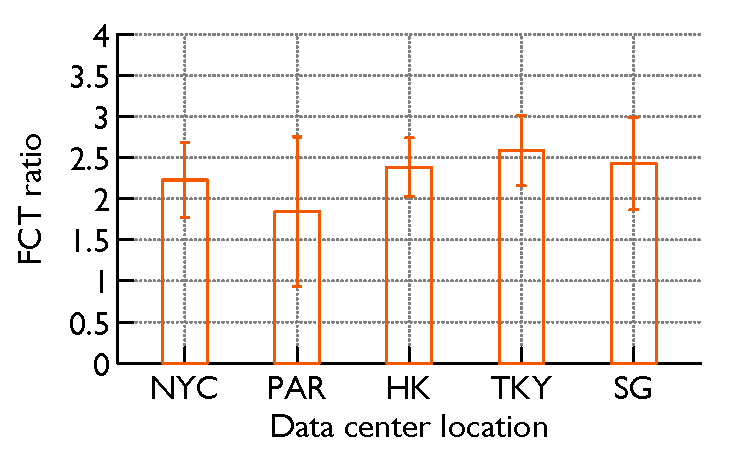
\includegraphics [width=0.23 \textwidth] {fig/c/compare-selected2.pdf}}
%       \subfigure[Bandwidth ratio]{
%        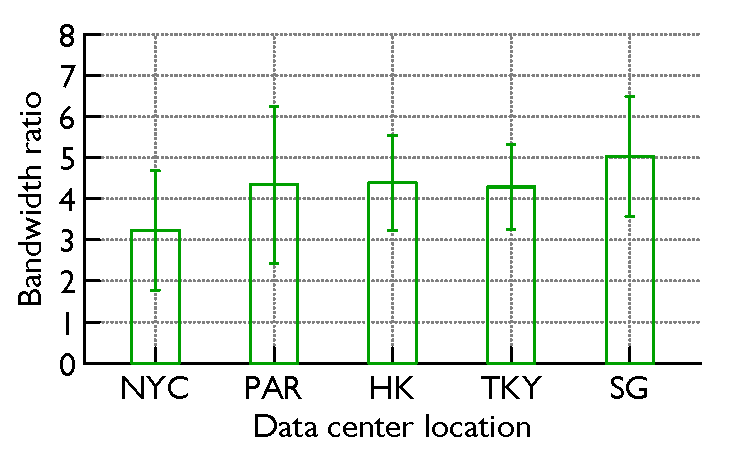
\includegraphics[width=0.23\textwidth]{fig/b/compare-selected.pdf}}
%     \caption{The Amazon inter-DC WAN performance.}
%    \label{wan-measure}
% \end{figure}

\section{Background and Motivation}\label{background}
In this section, we first briefly introduce network and common availability requirements in inter-DC WAN, then 
we use an example to demonstrate the limitations of state-of-the-art traffic engineering schemes in fulfilling such requirements.
%This section first shows the background.
%We then demonstrate the deficiencies of state-of-the-art traffic engineering schemes.

\subsection{Network failures and availability requirements}

%How to maintain high performance is a big problem for network operators.
%Frequent network failures can result in SLA violations and eventually loss of revenue to service providers \cite{riskbased,analysis-osdi,amazon,azure}.

\begin{figure*}[t]
\centering
\subfigure[Capacity and failure probability]{
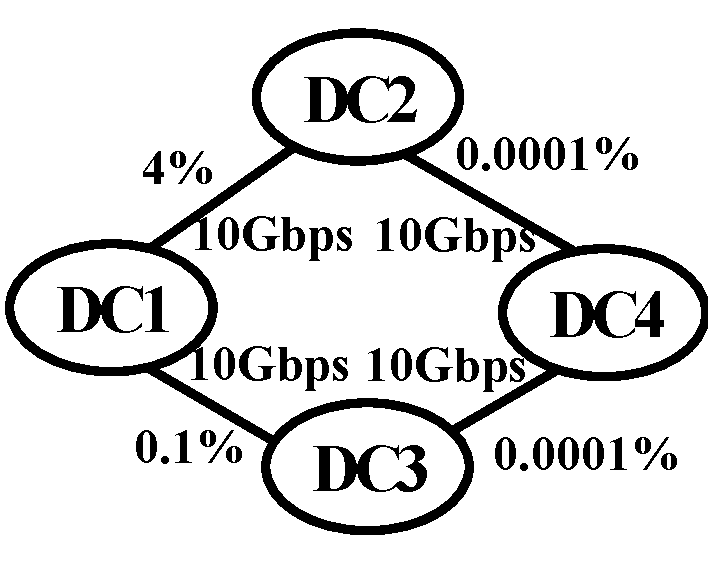
\includegraphics[width=0.24\textwidth]{fig/motivation-link.pdf}}
\subfigure[FFC (with one failure) ]{
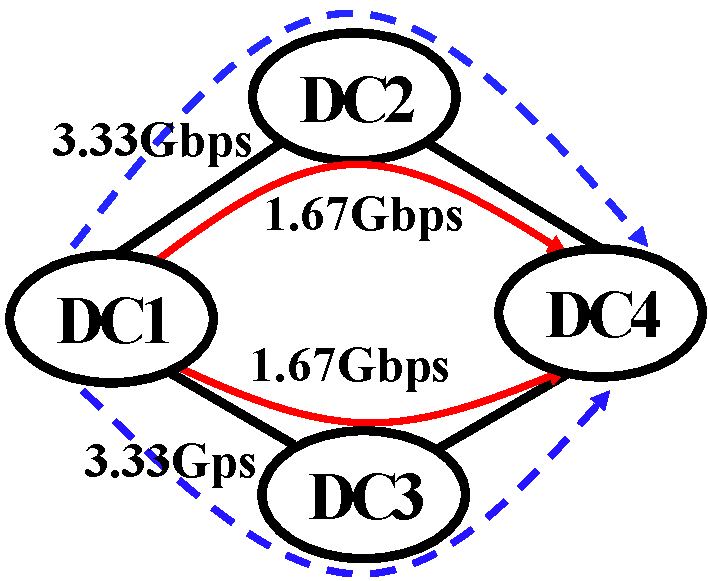
\includegraphics[width=0.24\textwidth]{fig/motivation-ffc.pdf}}
\subfigure[TEAVAR]{
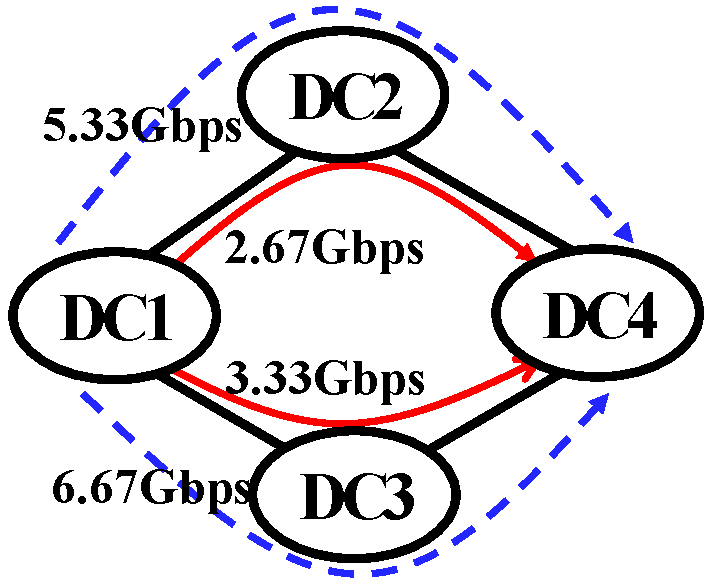
\includegraphics[width=0.24\textwidth]{fig/motivation-teavar.pdf}}
\subfigure[ $\mathsf{BATE}$]{
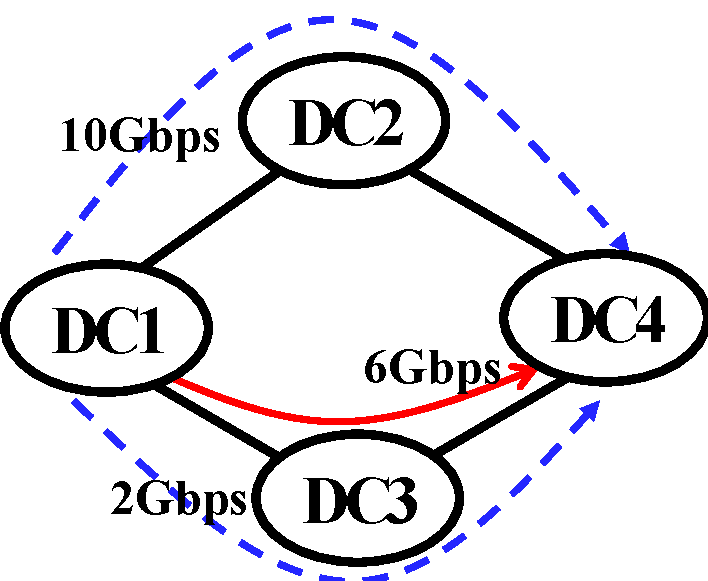
\includegraphics[width=0.24\textwidth]{fig/motivation-hate.pdf}}
\caption{A simple example where user1 (red) requires 6Gbps bandwidth for at least 99\% time and user2 (blue) requires 12Gbps bandwidth for at least 90\% time, both from DC1 to DC4. }%Link capacity is 10Gbps everywhere. Neither user gets enough bandwidth or availability guarantees under FFC or TEAVAR.  Both users are in line with their SLAs under $\mathsf{BATE}$. }
\label{motivatio_fig}
\end{figure*}

\begin{table}
\small
\centering
\caption{Services have different availability targets.}\label{target}
\renewcommand{\arraystretch}{1.0}
\begin{tabular}{|c|l|l|l|l|l|l|l|} \hline
\setlength{\tabcolsep}{10pt}
\textbf{Service}&\multicolumn{2}{|c|}{\textbf{Availability}}&\multicolumn{2}{|c|}{\textbf{Refund}}\\
\hline
{Traffic Manager \cite{azure}}&\multicolumn{2}{|c|}{$< 99.99\%$}&\multicolumn{2}{|c|}{$10\%$}\\
\hline
{VPN Gateway \cite{azure}}&\multicolumn{2}{|c|}{$< 99.95\%$}&\multicolumn{2}{|c|}{$10\%$} \\
\hline
{VM Instances \cite{amazon}}&\multicolumn{2}{|c|}{$< 99.99\%$}&\multicolumn{2}{|c|}{$10\%$} \\
\hline
{Cosmos DB \cite{azure}}&\multicolumn{2}{|c|}{$< 99.999\%$}&\multicolumn{2}{|c|}{$10\%$}\\
(Azure)&\multicolumn{2}{|c|}{$< 99\%$}&\multicolumn{2}{|c|}{25\%} \\
\hline
{DMS \cite{amazon2}}&\multicolumn{2}{|c|}{$< 99.99\%$}&\multicolumn{2}{|c|}{$10\%$}\\
(AWS)&\multicolumn{2}{|c|}{$< 99.0\%$}&\multicolumn{2}{|c|}{30\%}\\
&\multicolumn{2}{|c|}{$< 95\%$}&\multicolumn{2}{|c|}{100\%}\\
\hline
{AppFlow\cite{amazon3}}&\multicolumn{2}{|c|}{$< 99.99\%$}&\multicolumn{2}{|c|}{$10\%$}\\
(Amazon)&\multicolumn{2}{|c|}{$< 99.95\%$}&\multicolumn{2}{|c|}{25\%} \\
&\multicolumn{2}{|c|}{$< 95\%$}&\multicolumn{2}{|c|}{100\%} \\
\hline
{SMS\cite{alibaba3}}&\multicolumn{2}{|c|}{$< 95\%$}&\multicolumn{2}{|c|}{$10\%$}\\
(Alibaba)&\multicolumn{2}{|c|}{$< 90\%$}&\multicolumn{2}{|c|}{30\%}\\
\hline
{Data Transmission\cite{alibaba2}}&\multicolumn{2}{|c|}{$< 99.9\%$}&\multicolumn{2}{|c|}{$15\%$}\\
(Alibaba) &\multicolumn{2}{|c|}{$< 99.0\%$}&\multicolumn{2}{|c|}{30\%} \\
&\multicolumn{2}{|c|}{$< 95\%$}&\multicolumn{2}{|c|}{100\%} \\
\hline
\end{tabular}
\end{table}

\textbf{WAN failures are frequent and follow a heavy-tailed distribution.}
%Facing the growing scale and complexity of the WAN, how to maintain high availability is a challenge for data center network service providers\cite{evole, riskbased}. 
Failures could occur anywhere, from control plane to data plane across the network \cite{Teavar}.
They could also last for long durations, 
%Besides, failure events could be persistent with long durations.
as Google reports, more than 80\% of the failures last between 10 mins and 100 mins over their B4 network \cite{evole,riskbased}, 
%For some large failure events, before finding the root cause, they will try to drain services away from affected clusters \cite{evole}.
%The service resumption after such failures can even take one day, 
leading to severe performance degradation and revenue loss.
%Therefore, \textit{when planning for resource allocation, network risks should proactively be taken into consideration}.
On the other hand, 
according to the earlier measurements \cite{california,understanding}, failures often follow a \textit{heavy-tailed distribution},
where a small portion of links contribute to most of the failures, while most links experience only few failures, and the failure rate of
%Failure probability of 
a single link can differ by even more than three orders of magnitude \cite{failureslarge,Teavar}.
Therefore, \textit{network failures, especially their uneven distribution, should be explicitly taken into account by network operators}. 


\textbf{High availability directly translates into profit.}
Nowadays, high availability is nearly always one of the main items in SLAs  \cite{amazon,azure,amazon2}, and customers are eligible for a credit refund  if there are SLA violations. 
We conduct a survey on the SLA claims of different cloud providers, and Table \ref{target} shows their declared availability targets and  corresponding refunding policies,
%when violated.
%We can see that service providers often use a progressive piecewise function to derive refunding credits for violating availability targets. 
where the refunding credit is typically represented by a simple step function. 
For example, Microsoft Azure provides 10\% refund if its Traffic Manager service availability falls between 99.99\% and
99.0\%, and provides 30\% refund for anything below 99.0\% availability \cite{azure}. As more realtime and mission-critical applications (financial trading, online game, video streaming,
instant messaging, live broadcast, etc.) are deployed on the Internet, \textit{providing hard guarantee of high service availability under network failures to retain a good profit is a big challenge}.

%Maximizing network utilization and improving application availability are often contradictory.
%In tunnel-based TE mechanisms, when a failure occurs in a tunnel, the remaining available tunnels can be used to redistribute the traffic.
%%Therefore, some links might be overloaded.
%It is easy to see that the highly utilized networks are usually unable to accommodate traffic shifted from the failed tunnels. 
%%In order to maintain high availability service level, network capacity are always drastically over-provisioned for redundancy.
%However, low network utilization with substantially over-provisioned WAN capacity can lead to performance and profit loss. 
%%can degrade applications' performance and drastically over-provisioned WAN capacity for redundancy spends much money.
%It is a challenge to strike a balance between availability and performance.
%%These historical failures of links/nodes can reflect their reliability and be used in WAN resource allocation.
%%To guarantee links free from congestion, the network is proactively XXX.
%Therefore, \textit{some low failure-probability links can retain high utilization to guarantee the high throughput of applications, without necessarily leading to SLA violations}.



%\textbf{Inter-DC WAN is expensive:}
%Bandwidth on the Inter-DC WAN is valuable and important resource.
%According to one study of Microsoft, they even invest more than 100 millions of dollars on Inter-DC WAN.

%For example, Microsoft Azure network provider should guarantee their DNS queries will receive a valid response at least 99.99\% of the time, while  the availability demand of  Virtual WAN is  99.95\%.

%Therefore, providing adequate resources for each service can 



%
%\begin{figure*} 
%   \begin{minipage}[t]{0.48\linewidth} 
%         \subfigure[Insufficient bandwidth]{
%         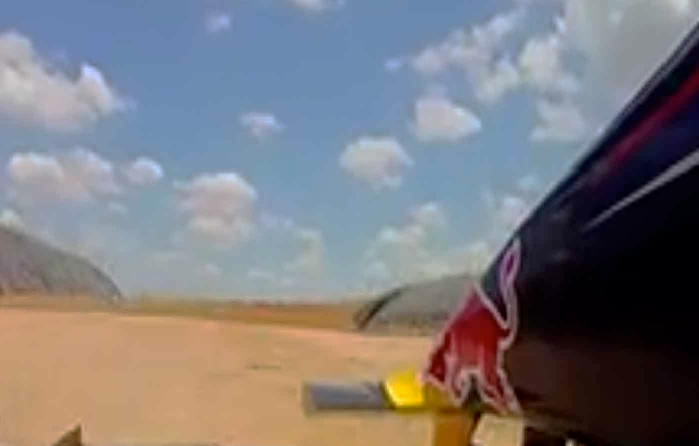
\includegraphics [width=0.45 \textwidth] {fig/motivation-1/1.pdf}}
%       \subfigure[Guarantee bandwidth]{
%        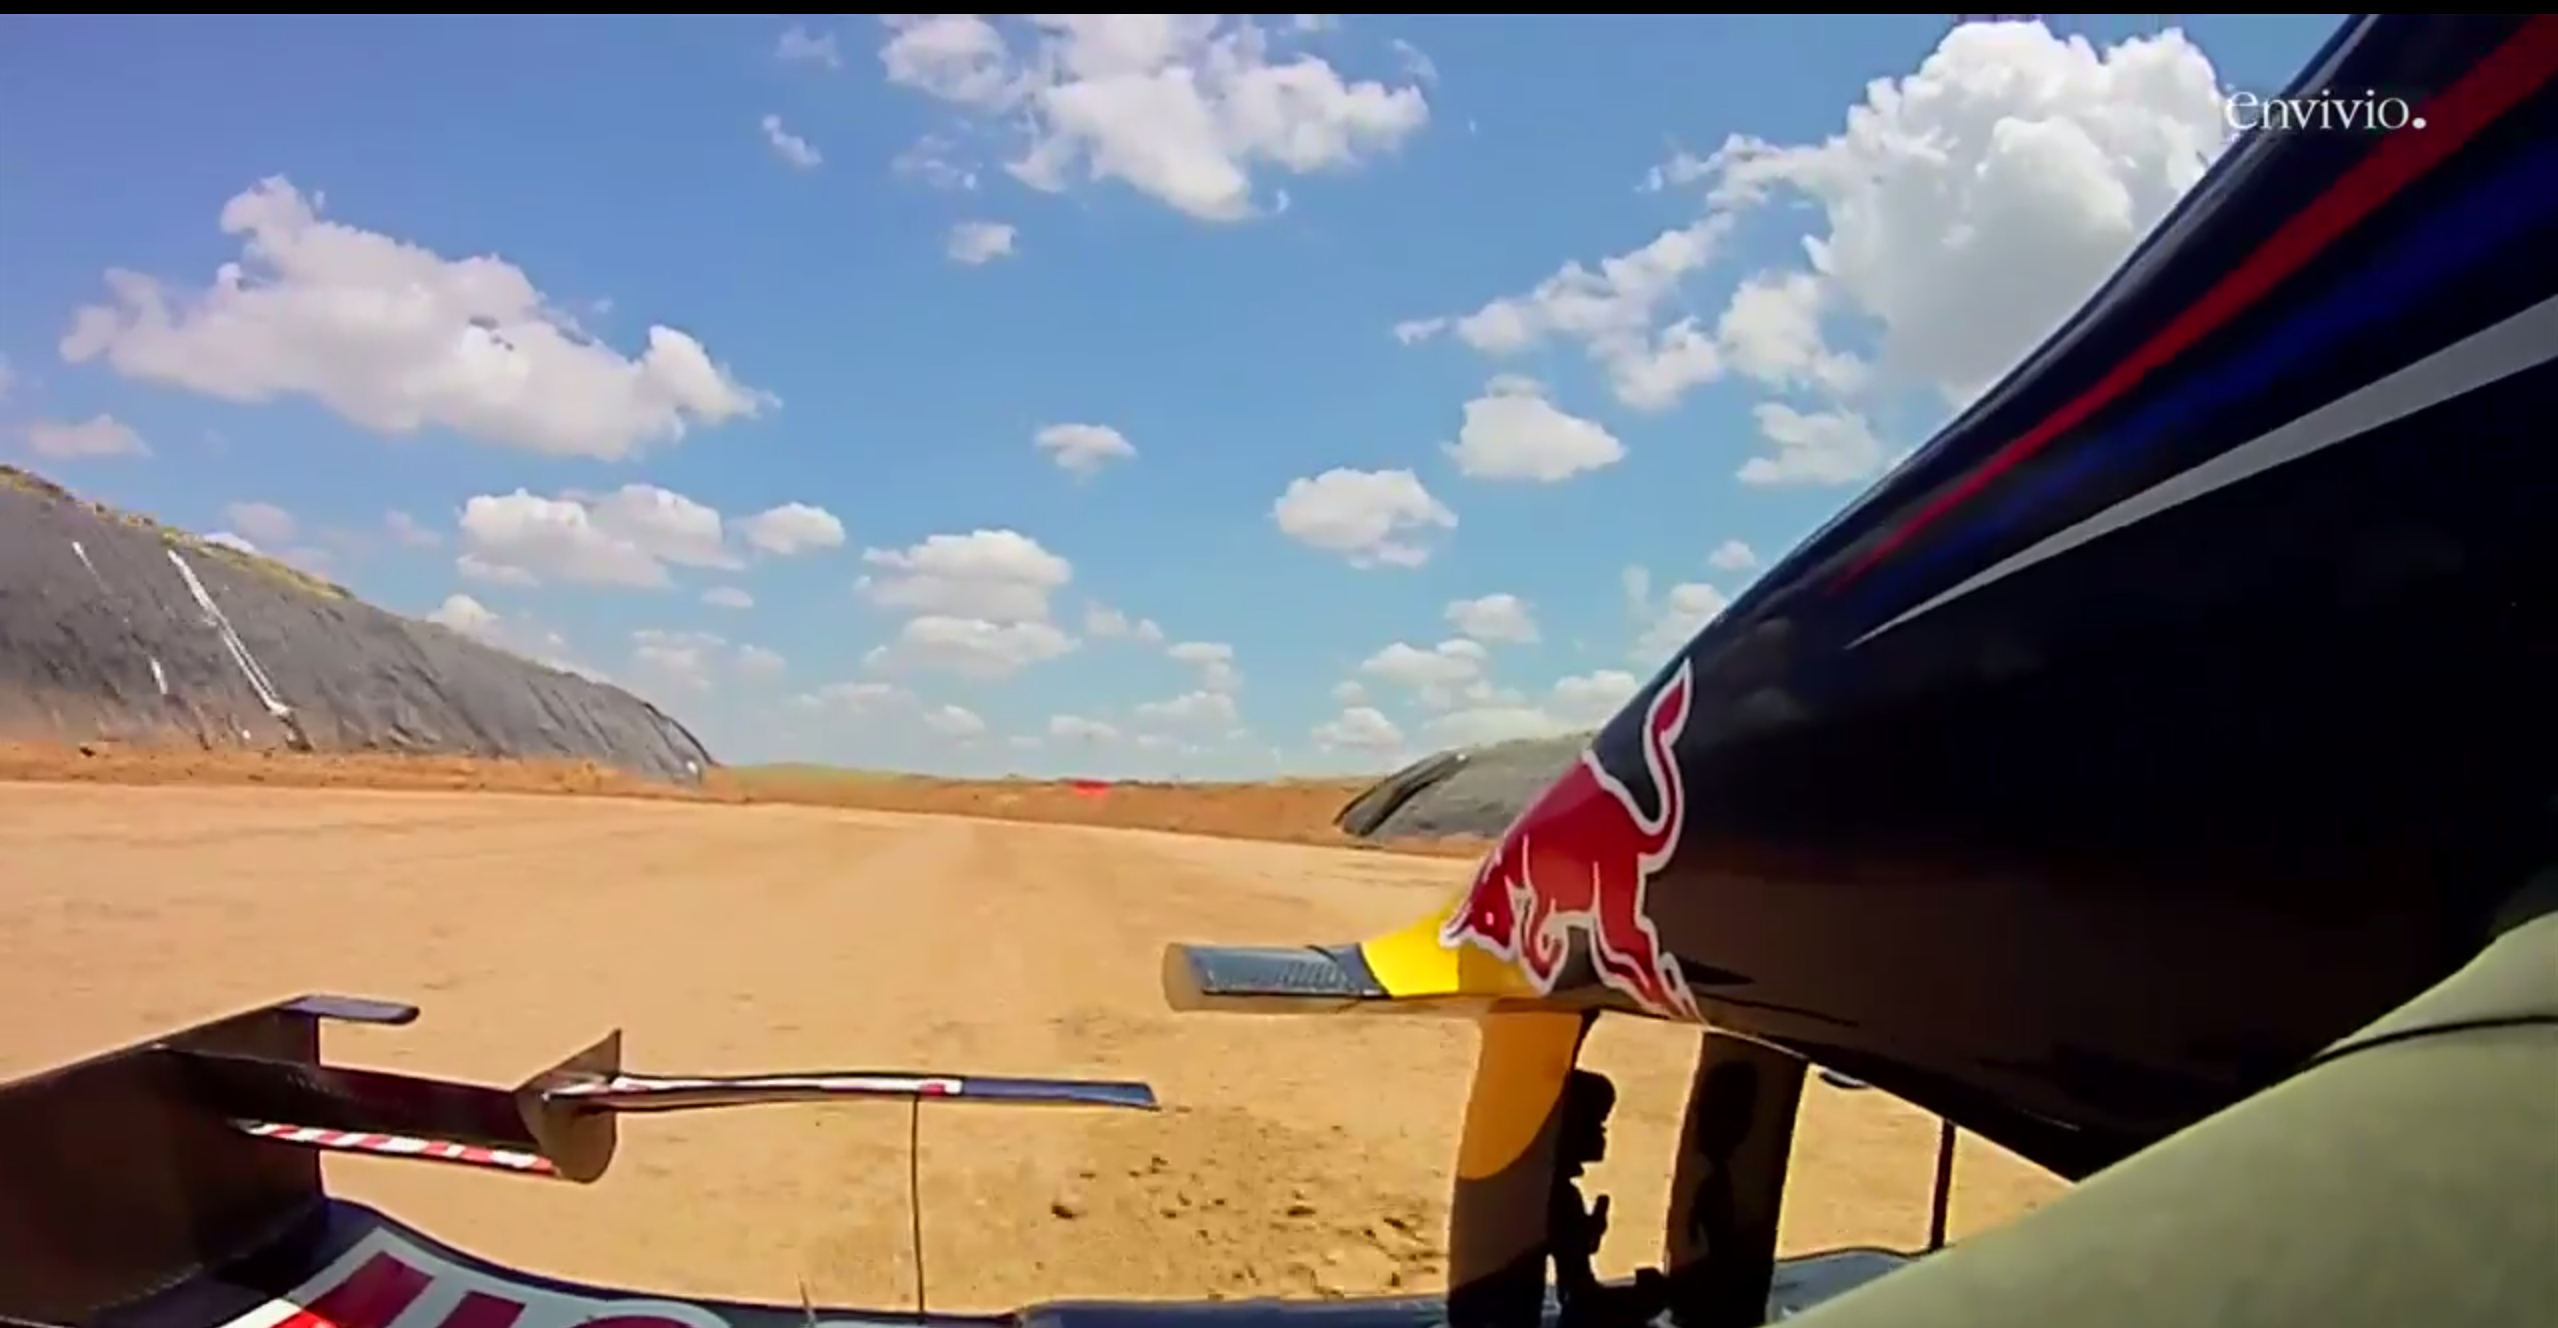
\includegraphics[width=0.45\textwidth]{fig/motivation-1/2.pdf}}
%     \caption{QoS comparison for the same video.}
%    \label{wan-measure-2}
% \end{minipage}% 
%  \begin{minipage}[t]{0.48\linewidth} 
%    \centering 
%       \subfigure[Completion time]{
%         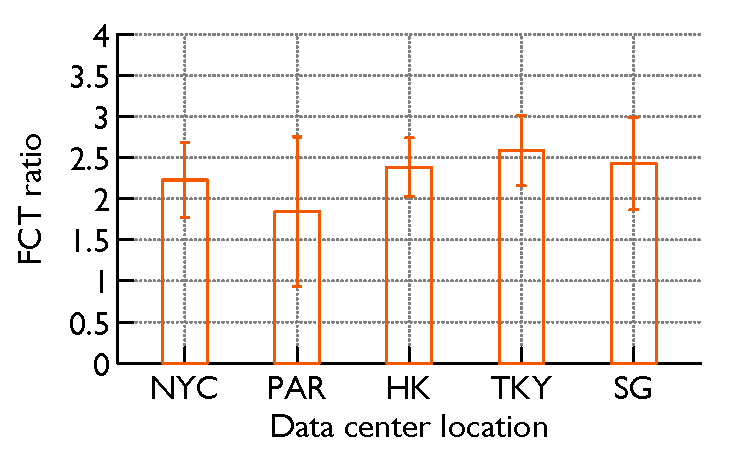
\includegraphics [width=0.48 \textwidth] {fig/c/compare-selected2.pdf}}
%       \subfigure[Bandwidth ratio]{
%        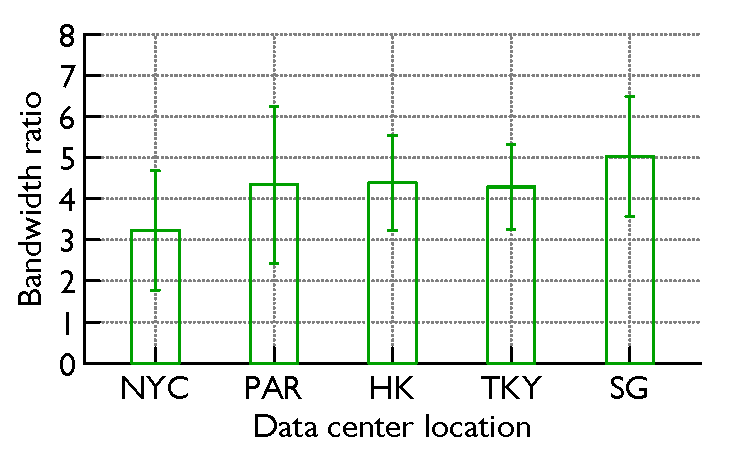
\includegraphics[width=0.48\textwidth]{fig/b/compare-selected.pdf}}
%     \caption{The Amazon Inter-DC WAN performance.}
%    \label{wan-measure}
%      \end{minipage}% 
%\end{figure*}










\textbf{A one-size-fit-all network availability target is not enough.}
%Availability has attracted major attention both in the industry and research community.
%Firstly, most of them only consider \textit{connectivity-based} availability\cite{hong2018b4}, which is conservative.
%The connectivity-based availability\cite{hong2018b4} is defined as the service uptime percentage, where a given minute is considered up if the connection is reachable and  it tries to quickly detour failed network devices, but \textit{they only focus on the reachability of networks and do not provide performance guarantees}.
%as a result, user experience might be influenced.
%Bandwidth on InterDC-WAN is a valuable resource and Microsoft \cite{swan} even spends millions of dollars on WAN investment.
In recent years, there has been a rapid increase in rapid and agile deployment of services over clouds.
Many studies have shown that users will quickly abandon sessions if the qualify of service is not guaranteed, leading to significant losses in revenue for content providers \cite{video1,video2,video3}.
Multiple services might be simultaneously launched over the global infrastructure operated by the same content provider or cloud provider. 
They might also pose different availability requirements, and  will contend for the  
% multiple service instances over different data centers globally at any time.
inter-DC WAN bandwidth.
% is a valuable resource and can become bottleneck \cite{swan} when  services \textit{contend} for network resource.
%In reality, availability targets vary with services, 
As shown in  Table \ref{target}, the minimal availability demands of the Data Transmission Service \cite{alibaba2} and the Short Message Service\cite{alibaba3} are 95\% and 90\%, respectively.
\textit{Such heterogeneous availability demands cannot be well captured and handled by a one-size-fit-all approach}, where all users get the same level of availability guarantee (e.g, TEAVAR  \cite{Teavar} only considers guaranteeing all users' bandwidth at least  $\beta\%$  time) . 
%Therefore, TEAVAR's guarantee such as "Users' bandwidth should be guaranteed at least $\beta\%$ time " \cite{Teavar}  is not enough,
%since it fails to differentiate availability targets of services.

%Traditionally, the availability is defined as the service uptime percentage, where a given minute is considered up if the connectivity is successful.
%We call this connectivity-based availability.
%%individual services have vastly different bandwidth, latency and loss requirements.
%\textit{The connectivity-based availability is insufficient since it only emphasizes on the success of connectivity but can't guarantee bandwidth demands and QoE will drop significantly if minimal bandwidth is unable to be provisioned}.
%However, modern public cloud providers can't always guarantee applications' bandwidth over their inter-DC WAN.
%We perform measurement on Amazon global inter-DC WAN to prove this.
%We select 6 data centers: NYC (US east), PAR (Europe), HK (Asia Pacific), TKY (Asia Pacific), SG (Asia Pacific), London (Europe).
%In each data center, we purchase one VM with high network performance metric. 
%We transfer 5GB data from London to other VMs at different times and Figure  \ref{wan-measure} (a) shows ratio of maximal and minimal flow completion time. 
%We can see the FCT variation can even be as large as 3 $\times$.
%To investigate this problem, we next start TCP connections from London to other data centers and compute the ratio of maximal bandwidth and minimal bandwidth every 10 minutes.
%The measurement lasts one day and Figure \ref{wan-measure} (b) demonstrates the result.
%We can see that bandwidth ratio varies from 2 to 7, which suggests the inter-DC WAN is unable to ensure the timely data delivery of online services.


%The way of transmitting bandwidth utilizes redundant resources. 
%However, without proper resource allocation, when an error occurs in a certain path, even if the switch quickly detects the error and expands the bandwidth on other backup paths, it will cause congestion in the expanded network, which will affect the performance of the application. 
%Current network operation and maintenance personnel can calculate the error probability of each link based on . 
%. , Can jointly optimize network utilization and availability.

%
%Most current data center WAN resource allocation mechanisms focus on improving network resource utilization, or optimizing the performance of data center WAN, and rarely consider how to provide continuous and uninterrupted service guarantee for applications. 
%At present, although there have been a series of work in resource allocation, considering the availability requirements of network services, but there are some problems, we will introduce in the next section.






\subsection{A motivating example for $\mathsf{BATE}$}
Now we use a simple example to illustrate why existing traffic engineering algorithms cannot 
meet the heterogeneous bandwidth availability demands well. The toy topology we use is depicted 
in Figure \ref{motivatio_fig}(a), where there are 4 data centers and the links connecting them 
are annotated with their corresponding capacities and failure probabilities. Suppose we have two 
bandwidth demands for inter-DC transmission from DC1 to DC4, i.e., user1 (red) requires 6Gbps bandwidth 
with at least 99\% availability, and user2 (blue) requires 12Gbps bandwidth with at least 90\% availability. 
There are two paths from DC1 to DC4, i.e., DC1$\to$ DC2 $\to$ DC4, and DC1 $\to$ DC3 $\to$ DC4, whose available probabilities are $(1-4\%) \times (1-0.0001\%)=95.999904\%$ and $(1-0.1\%) \times (1-0.0001\%) = 99.8999001\%$, respectively. We apply FFC \cite{FFC} and TEAVAR \cite{Teavar}, two latest WAN traffic engineering schemes that take network failures into account, to this scenario. 

FFC \cite{FFC} guarantees a total bandwidth from DC1 to DC4 under at most $l$ concurrent node/link failures, and here we simply use $l=1$. Figure \ref{motivatio_fig}(b) shows FFC can support 10Gbps bandwidth from DC1 to DC4 in 99.996\% time even with one failure (the probability that the two paths fail simultaneously is $(1-95.999904\%) \times (1-99.8999001\%) = 0.004004092096\%$). Since user1 and user2 can get respectively 3.34Gbps and 6.66Gbps, which are evenly distributed on the two paths from DC1 to DC4, 
and neither of their bandwidth demands can be satisfied. This shows \textit{FFC does not differentiate between paths with different availabilities.} The lower path has a much smaller failure probability, and it is wasteful without utilizing it as much as possible. 

On the other hand, TEAVAR \cite{Teavar} exploits the different link failure probabilities and maximizes the network utilization, subject to meeting a \textit{single} desired availability. Figure \ref{motivatio_fig}(c) illustrates the bandwidth allocation result of TEAVAR, where user1 and user2 can get their demanded 6Gbps and 12Gbps bandwidth, both in about 95.9\% time. However, this falls below 
user1's availability demand, i.e., 99\%, and will cause a SLA violation. 
This shows  \textit{TEAVAR does not consider the heterogeneous user demands on availability.} 
Since user1 requires a higher availability, it is better to use a path with a lower failure probability. 

\iffalse
FFC \cite{FFC} seeks to assign a total bandwidth $f_k$ to each node pair $k$.
It achieves this by reserving bandwidth on each tunnel between $k$ and ensuring the total bandwidth of all tunnels is larger than $f_k$ under $l$ concurrent node/link failure scenarios.
TEAVAR \cite{Teavar} ensures that all scenarios meeting bandwidth demand $d_k$ has a total probability no less than the required availability target.
%considers the probability of each scenario and regards the sum of the probabilities for scenarios where bandwidth demand $d_k$ between each node pair $k$ is fully satisfied as the achieved availability.
TEAVAR maximizes the network utilization subject to meeting a \textit{single} desired availability target (e.g., 99.99\%).
In this part, we demonstrate that reasoning about  availability in terms of
the number of concurrent failures is often too conservative while meeting the same availability target for diverse services is often not enough.
%FFC\cite{FFC} uses the concurrent node/link failures as the proxy for availability;
%TEAVAR\cite{Teavar} tries to leverage the financial risk theory and optimize bandwidth allocation subject to meeting a desired availability target (e.g., 99.99\%).
%In this part, we will use a simple example to demonstrate the flaws of FFC and  TEAVAR.


Figure \ref{motivatio_fig}(a) shows a network topology, where DC1 is connected to DC4 via DC3 and DC2.
The capacity of each link is 10Gbps and we also show the link failure probability in this figure.
There are two paths from DC1 to DC4:
(1) DC1$\to$ DC2 $\to$ DC4, (2) DC1 $\to$ DC3 $\to$ DC4, whose available probabilities are 95.999904\% (i.e., 96\% $\times$ 99.9999\%) and 99.8999001\% (i.e., 99.9\% $\times$ 99.9999\%).
%We can derive the uptime fraction of path $(1)$ and $(2)$, i.e., 95\% and 99\%, respectively.
%There are two tenants, where tenant1 (red) deploys service1 with 6Gbps bandwidth demand from DC1 to DC4 and tenant2 (blue) deploys service2 with 12Gbps bandwidth demand from DC1 to DC4
There are two services deployed by a tenant, where service1's (red) minimal bandwidth demand of 6Gbps from DC1 to DC4 should be guaranteed at least 99\% time and service2's (blue) minimal bandwidth demand of 12Gbps from DC1 to DC4 should be guaranteed at least 90\% time.
%whose bandwidth demands are 6Gbps and 12Gbps.
%Availability demands of App1 and App2 are  99\% and 90\%, respectively.
%Assume App1 and App2 need to maintain the minimal bandwidth demands 99\% and 90\% time.
%App1's  is  with availability SLO target and App2's bandwidth demand is  with  availability SLO target.
%We take FFC-1 that can tolerate one network failure as the example and Figure \ref{motivatio_fig}(b) demonstrates the allocation result.
We demonstrate the bandwidth allocation under FFC-1 scheme (which can tolerate one network failure) in Figure \ref{motivatio_fig}(b).
We can see that FFC can support total 10Gbps bandwidth almost 99.9999\% time (unless path (1) and (2) fail simultaneously), where service1 and service2 can gain 3.34Gbps and 6.66Gbps, respectively.
%Indeed, 10Gbps can be guaranteed unless path (1) and (2) fail simultaneously.
Neither service is able to get enough bandwidth, because FFC treats the two paths indifferently without their individual failure rates.
However, path (2) has much smaller failure probability and lowing its utilization does not help improve availability and is wasteful.
TEAVAR exploits the different failure probability of network and advocates to fully utilize links under a loss-based availability target constraint (e.g., 99\%).
%Given the availability target 99.9\%, Figure \ref{motivatio_fig}(c) demonstrates the solution of TEAVAR.
TEAVAR's solution, shown in Figure \ref{motivatio_fig}(c), can guarantee service1 and service2 attaining 6Gbps and 12Gbps about 95.9\% time.
TEAVAR fails to satisfy availability target of service1, since it allocates network resources under a single availability target and ignores the different expectations of the two services.
As a result, it can't meet service1's availability demand.
%This suggests that TEAVAR ignores demands of different applications, as a result,  applications with higher availability demands might be unable 
\fi

\textbf{Our approach:}
%$\mathsf{BATE}$ exploits network failure probability and attempts to satisfy applications'  bandwidth-based availability demands.
Taking into account the diverse link failure probabilities and user bandwidth availability demands, 
Figure \ref{motivatio_fig}(d) shows a better bandwidth allocation, 
where user1 can get 6Gbps over 99.8999001\% time (via the lower path that has a lower failure probability) and user2 can get 12Gbps over 95.999904\% time (via both the upper and the lower path), 
satisfying both of their bandwidth demands. 

%The minimal bandwidth demands of applications are able to be met with high probability under $\mathsf{BATE}$.
%Low failure probability links are fully utilized to satisfy the high availability demands of applications.
%We elaborate the details of $\mathsf{BATE}$ in the following section.



\begin{table}[h!]
\small
\centering
\caption{Key Notations for $\mathsf{BATE}$}\label{Notation}
\renewcommand{\arraystretch}{1.0}
\begin{tabular}{ccccccc}  \toprule \toprule 
\setlength{\tabcolsep}{5pt}
&\textbf{Input Variables}\\
\hline
$G(V,E)$ &\multicolumn{6}{|l}{inter-DC WAN with nodes $V$ and Links $E$}\\
\hline
$c_e$ &\multicolumn{6}{|l}{the remaining capacity on link $e \in E$}\\
\hline
$k\in K$ &\multicolumn{6}{|l}{a s(ource)-d(estination) pair in the set of all s-d pairs}\\
\hline
$T_{k}$ &\multicolumn{6}{|l}{the set of tunnels for a s-d pair $k$}\\
%\multirow{3}{*}{VM Instances}&\multicolumn{2}{|c|}{$< 99.99\%$}&\multicolumn{2}{|c|}{$10\%$}&\multirow{3}{*}{Azure}\\
%&\multicolumn{2}{|c|}{$< 99\%$}&\multicolumn{2}{|c|}{25\%}& \\
%&\multicolumn{2}{|c|}{$< 95\%$}&\multicolumn{2}{|c|}{100\%}& \\
\hline
$D, D_a$&\multicolumn{6}{|l}{the set of arrived demands and admitted demands\footnote{When an admitted demand finishes, it will be removed from $D_a$.} }\\
\hline
\multirow{3}{*}{$d=(\mathbf{b}_d, \beta_d)$}&\multicolumn{6}{|l}{for a BA demand $d$, requiring bandwidth $\mathbf{b}_d$ with }\\
&\multicolumn{6}{|l}{ availability $\beta_d$, where $\mathbf{b}_d$ is a vector $<\mathbf{b}^1_d, \mathbf{b}^2_d, ...>$}\\
&\multicolumn{6}{|l}{of bandwidth demands over all s-d pairs\footnote{Here we omit the start and end time of this demand, but they will be implicitly considered in our online admission and traffic scheduling.}} \\
%$d_i=(\mathbf{b_i}, \beta_i)$ &\multicolumn{6}{|l}{the $i$-th user demand, requiring bandwidth $\mathbf{b_i}$ with availability $\beta_i$, where $\mathbf{b_i}$ is a vector $<\mathbf{d}_i^1, \mathbf{d}_i^2, ...>$ of bandwidth demands over all s-d pairs\footnote{Here we omit the start and end time of this demand, but they will be implicitly considered in our online admission and scheduling.}}\\
%\hline
%$D, D_a$&\multicolumn{6}{|l}{the set of arrived demands and admitted demands\footnote{$D_a$ will update every time slot and an admitted demand will be removed if it finishes.} }\\
%\hline
% $j\in J$ &\multicolumn{6}{|l}{the $j$-th availability target in the level set}\\
%\hline
%$\mathbf{b}^k_d$ &\multicolumn{6}{|l}{Bandwidth demand through node pair $k$ of $i$}\\
%\hline
%$\gamma_{i}$ &\multicolumn{6}{|l}{Service type (i.e., $j$) of demand $i$}\\
%\hline
%$ \beta_{j}$ &\multicolumn{6}{|l}{Bandwidth-based availability target of service $j$}\\
\hline
$t$ &\multicolumn{6}{|l}{a tunnel for transmitting traffic\footnote{Multiple tunnels may exist for a single s-d pair.}}\\
\hline
$u_t^e$ &\multicolumn{6}{|l}{whether tunnel $t$ passes link $e \in E$}\\
\hline
$\bm{z}\in \bm{Z}$ &\multicolumn{6}{|l}{a failure scenario in the scenario set}\\
\hline
$p_{\bm{z}}$ &\multicolumn{6}{|l}{the probability that a failure scenario $\bm{z}$ occurs}\\
\hline
$v_t^{\bm{z}}$ &\multicolumn{6}{|l}{whether tunnel $t$ is available under scenario $\bm{z}$}\\
 \hline
% $\{1,\beta_j^1,\beta_j^2....\}$ &\multicolumn{6}{|l}{The availability target list for service $j$}\\
%  \hline
% $\{1,\alpha_j^1,\alpha_j^2...\}$ &\multicolumn{6}{|l}{The profit list for service $j$}\\
\hline

&\textbf{Output Variables}\\
\hline
$g_d$& \multicolumn{6}{|l}{whether demand $d$ is admitted}\\
\hline
%$f_{d}^t$& \multicolumn{6}{|l}{bandwidth allocated for the $i$-th demand over tunnel $t \in T_{k}$ }\\
$f_d^t$& \multicolumn{6}{|l}{bandwidth allocated for demand $d$ over tunnel $t$}\\
\hline
$h_d$& \multicolumn{6}{|l}{profit (after refunding)  for demand $d$}\\
%\hline
%\hline
%&\textbf{Auxiliary Output Variables}\\
%\hline
%% $S_j$ &\multicolumn{6}{|l}{Network service achieved availability of $j$}\\
%%\hline
% $A_d^{\bm{z}}$&\multicolumn{6}{|l}{Whether scenario $\bm{z}$ is safe or not for $i$ }\\
% \hline
% $S_i$&\multicolumn{6}{|l}{Achieved availability of $i$ }\\
\bottomrule
\bottomrule
\end{tabular}
\end{table}

\section{$\mathsf{BATE}$ framework}\label{HATE}
In this section, we discuss the details of $\mathsf{BATE}$, which contains three parts, i.e., admission control, traffic scheduling and failure recovery, using notations summarized in Table \ref{Notation}. 
The framework intends to achieve the following objectives: 
 \begin{itemize}
\item \textbf{High admission ratio and low admission latency:}  
  Bandwidth availability demands might arrive at anytime. 
  The system should be able to efficiently accommodate as many BA demands as possible under the constraint of network capacity and failure probabilities, as this would increase service agility and bring more revenue. %availability and bandwidth targets.
\item \textbf{High availability for allocated bandwidth:}
The system should be able to optimize its achieved availability in a probabilistic manner, 
as this would, in the long term, reduce potential penalties (i.e., refund due to SLA violations) and retain a good reputation. This can be achieved by making a good match between demands on higher availability and paths with low failure probability.
%make services with stringent availability requirements (e.g., 99.999\%) pass links with high reliability.
%Therefore, their bandwidth demands can be guaranteed with high probability.
\item \textbf{Automatic and economical failure recovery:}
If any link failure really happens, the system should reroute traffic away from that link, 
while minimizing any possible collateral damage to normal traffic, i.e., congestion and lower bandwidth availability due to rerouting.
%\item \textbf{ \& scalability:}
%
\end{itemize}

\subsection{Abstraction of bandwidth availability demands}
%Recently, deploying multiple virtual private clouds over public clouds (e.g., Amazon AWS) or deploying multiple services over private clouds (e.g., Google internal DCs) is becoming  a common practice for content providers.
%Tenants could deploy diverse service instances over Inter-DC WAN.
In reality, a customer could be a tenant who launches multiple virtual private clouds over  multiple DCs in public clouds (e.g., Amazon AWS) or could be a service team who launches multiple VM instances in private clouds (e.g., Google internal DCs).
%The cloud providers are providing many services and each service contains numerous instances across geo-distributed data centers.
%For example, a common practice is running MapReduce operations across geo-distributed data centers and many connections from mappers to reducers are maintained.
%Services have different bandwidth demands as well as availability targets.
However, there exists no interface for tenants to specify bandwidth availability.
We now present $\mathsf{BATE}$ 's availability abstraction.

\textbf{BA demand model:}
We model the inter-DC WAN as a  graph $G=(V,E)$,  where $V$ and $E$ are nodes and link sets.
Let $K$ denote the a source and destination DC pair.
%Each link $e\in E$ is associated with a link capacity $c_e$ (e.g., in bps).
%DC pair set is $K$ and  $\beta_j$ presents the desired availability target  of service $j \in J$.
%\multirow{3}{*}{$d_i=(\mathbf{b}_i, \beta_i)$}&\multicolumn{6}{|l}{the $i$-th user demand, requiring bandwidth $\mathbf{b}_i$ with }\\
%&\multicolumn{6}{|l}{ availability $\beta_i$, where $\mathbf{b}_i$ is a vector $<\mathbf{b}_i^1, \mathbf{b}_i^2, ...>$}\\
%&\multicolumn{6}{|l}{of bandwidth demands over all s-d pairs\footnote{Here we omit the start and end time of this demand, but they will be implicitly considered in our online admission and traffic scheduling.}} \\
For a  bandwidth availability demand $d$, the BA abstraction can be presented as $(\mathbf{b}_d, \beta_d,t_d^s,t_d^e)$,
where $\mathbf{b}_d$ is a vector $<\mathbf{b}_d^1, \mathbf{b}_d^2, ...>$ of bandwidth demands over all s-d pairs.
%where $\alpha$ and $\delta$ are the arrival and departure of the demand, $\gamma$ denotes the service type and $\theta =\{d_{1}, d_{2}, ...,d_{K} \}$ presents bandwidth over each node pair.
%We assume one tenant can only start one service and if a tenant wants to boot multiple services, we can use multiple tuples to describe it.
Network providers will offer refunding for any violating availability targets (see $\S$\ref{background}) and we use $h_d$ to denote the profit (after refunding) for demand $d$.
%The system should reserve enough bandwidth to guarantee all \textit{admitted} requests' availability demands.
%When all services'  \textit{achieved} bandwidth-based availability are larger than their corresponding desired availability target, the system is able to accommodate this service request, otherwise, the request will be denied.

%If the achieved availability (i.e., $S_j$) is larger than the highest desired availability target (i.e., $\beta_j^1$), the profit is 1.


\textbf{Network  model:} 
%$\mathsf{BATE}$ relies on network operators to provide link failure probabilities.
%A series of failure events (e.g., power outage, configuration mistakes, firmware bugs) directly lead to link failures.
%%According to the report of Google \cite{evole}, more than 90\% of the failure events can lead to high packets losses, or blackholes to entire data centers and they might occur anytime.
%Operators maintain the network empirical data, which can be used to estimate the link risks\cite{jointfailure,overview,evole}.
%For each link $e$, operators can examine historical data and track whether $e$ was up or down in a measured time epoch (e.g., 1min).
%The link up probability $p_i$ of link $i$ can be given by the up epoch percentage and its failure probability is $1-p_i$.
%Inspired by the site reliability engineering (SRE) technology\cite{jointfailure,overview}, we propose a general failure model.
A network scenario $\bm{z}=\{z_1,z_2,...\}$ is a vector consisting of each link's state.
Each element $z_i \in \{0,1\}$ denotes whether link  $i$  is up ($z_i=1$) or down  ($z_i=0$).
%Operators maintain the network empirical data, which can be used to estimate the link risks\cite{jointfailure,overview,evole}.
For each link $e$, operators can examine historical data and track whether $e$ was up or down in a measured time epoch (e.g., 1 min).
The up probability $p_i$ of link $i$ can be given by the up epoch percentage and its failure probability is $1-p_i$.
Let $\bm{Z}$ present the network scenario set and $p_{\bm{z}}$ is the probability of scenario $\bm{z}\in \bm{Z}$.
%Each link is up with the probability of $p_i$. \cite{Teavar}
Let $z_i'$ denote the value of $z_i$, and assume link failures are independent.
Similar to TEAVAR \cite{Teavar},  probability of network scenario  $\bm{z}$ is given by:

\begin{eqnarray} \label{state}
p_{\bm{z}}&=&p\left( z_1=z_1',z_2=z_2',z_3=z_3',...,z_{e}=z_{e}'\right)\nonumber \\
&=&\prod_{i=1}^{|E|}(z_i'p_i+(1-z_i')(1-p_i))
\end{eqnarray}

For example, an inter-DC WAN contains three links $E=\{e_1,e_2,e_3\}$. 
Network scenario $\{1,1,0\}$ means $e_1$ ,$e_2$ are available and  $e_3$ fails.
If the up probability of $e_1,e_2,e_3$ are 0.9, 0.8, 0.85, respectively.
Then its probability $p(\{1,1,0\}) =0.9\times0.8\times0.15=0.108$.


We consider tunnel-based forwarding \cite{FFC,swan,Teavar}, where traffic is carried over a set of tunnels.
%Consider an undirected graph $G = (V,E)$ and a set of $k$ pairs: $s_1t_1, s_2t_2,..., s_kt_k$,
For each node pair $k\in K$ of the inter-DC WAN, we are given a set of pre-selected tunnels $T_{k}$, where tunnel set $T_{k}$ can be derived with different routing schemes (e.g., k-shortest paths, edge disjoint paths \cite{Bruno2013Dynamic}, oblivious routing \cite{SMORE}). 
%In Section \ref{evaluation}, we evaluate the impact of routing schemes  on performance.
Each tunnel $t\in T_{k}$ contains a set of links and  $u_t^e$ presents whether tunnel $t$ contains link $e\in E$ or not.
%The network scenario set is $\bm{Z}$ and the corresponding probability is $p_{\bm{z}}, \forall \bm{z}\in \bm{Z} $.
$f_d^t$ is the bandwidth allocated over tunnel $t$ for demand $d$ and 
$D_a$ is the total \textit{admitted} demand set.
Let $v_t^{\bm{z}}$ denote whether tunnel $t$ is available (i.e., $v_t^{\bm{z}}=1$)  or not  (i.e., $v_t^{\bm{z}}=0$) under network scenario $\bm{z}$.

%\begin{enumerate}
%    \item  How to accommodate as many requests as possible subject to network failure model and diverse service availability targets  (see $\S$ \ref{admission_control}).
%    \item  How to route all admitted requests with minimum induced network overload under the constraint of network failure model and diverse service availability targets (see $\S$ \ref{TE}).
%    \item  How to reroute requests with minimum cost when network fails (see $\S$ \ref{backup}).
%\end{enumerate}

%\subsection {Modeling network scenarios}
%%We now discuss how to model network failure scenarios.


%Under network scenario $\bm{z}$, a tunnel $t$ is available only when all the links it passes by are up.



%Consider a set of failure event set $H$ can influence the network reliability.
%If an event $h\in H$ occurs, the network device will become unavailable.
%Similar to \cite{Teavar}, we also assume all the events are uncorrelated and use $p_h$ to denote the probability of occurrence for event $h$.
%Vector $\bm{q}=\{q_1,q_2,...,q_{|H|}\}$ denotes one state, where $q_h\in \{0,1\}$ presents whether event $h$ will happen($q_h=1$) or not ($q_h=0$).
%$q_h'$ is the value of $q_h$.
%The probability of state $\bm{q}$ can be derived from the occurrence probability of events:
%
%\begin{eqnarray} \label{q}
%p(\bm{q})&=&p\left( q_1=q_1',q_2=q_2',q_3=q_3',...,q_{h}=q_{h}'\right)\nonumber \\
%&=&\prod_{h\in H}(q_h'p_h+(1-q_h')(1-p_h))
%\end{eqnarray}
%
%For instance,  we consider four events $H=\{h_1,h_2,h_3,h_4\}$ for link $e$.
%The occurrence probability of the four events are $p_{h_1}=0.2, p_{h_2}=0.3,p_{h_3}=0.4,p_{h_4}=0.5$, respectively.
%$\bm{q}=\{1,0,0,0\}$ presents only event $h_1$ happens.
%Then the probability of state $\bm{q}$ is: $p(\bm{q})=0.2\times0.7\times0.6\times 0.5=0.042$.
%Consider all events will not happen, we can also derive the available probability of link $e$: $p(\{0,0,0,0\})=0.8\times0.7\times0.6\times 0.5=0.168$.


%\subsection {Traffic Engineering for Diverse Availability Targets }\label{BATE}
%Based on the the network scenarios, we design our traffic engineering algorithm that optimizes bandwidth-based availability for diverse services.
%To this end, we introduce the problem formulation of $\mathsf{BATE}$ problem and 

\subsection {Admission control} \label{admission_control}
Users' demands arrive in the first-come-first-service (FCFS) manner and \textit {no preemption} is allowed.
The new arrival demand, together with the admitted ones (i.e., $D_a$), constitute demand set $D$.
%The Admission control  \textit{determines whether availability target of $\forall d \in D$ can be supported simultaneously subject to network failure model}.
%If this is true, the new arrival demand can be admitted, otherwise, it is rejected.
If every element in $D$ can meet its availability target, the new arrival demand can be admitted, otherwise, it is rejected.
To accommodate as many demands as possible, we can model the admission control as a 0-1 Mixed-Integer Linear Programming (MILP) and maximize the number of demands that satisfy availability targets.
Appendix \ref{admission_problem} shows the optimization formulation.
The admission control optimization problem can be proven as a NP-hard problem by reducing the all-or-nothing multi-commodity flow problem \cite{inproceedings2} to a special case of it.
We omit the details for brevity.
%If availability target of $\forall d \in D$ can be supported simultaneously subject to network failure model, the new arrival demand can be admitted, otherwise, it is rejected.
%If , we can model the 
%The Admission control part decides whether a new demand submitted by a tenant can be admitted or not.

%Solving the optimization problem shown in Appendix \ref{admission_problem} can determine whether the new coming tenant's demand can be admitted.
%However,  the large size of network scenarios and 
In reality, 
%tenants' demands can arrive at anytime and admission control should reply to the tenants in near real time.
there is a \textit{tradeoff} between efficiency and optimal solution:
If we assume all the admitted demands are fixed and can't be rescheduled, then we can derive the solution fast but the new arrival one might be unable to be accommodated;
If we derive the optimal solution  by solving the optimization problem shown in Appendix \ref{admission_problem}, then we can accommodate more demands, however, this is time-consuming.
To achieve a tradeoff, we would like to address the following three steps:

\begin{enumerate}
    \item When a new demand $d$ arrives, we assume that all admitted demands are \textit{fixed} and check whether the remaining network capacity and the corresponding links' up probability can support it. If this is true, then go to step (3), otherwise, go to step (2).
    \item Run Algorithm \ref{greedy-1}  and check whether all admitted demands can be rescheduled to accommodate the new arrival demand $d$. If this is true, then go to step (3), otherwise, the system will reject the demand, which can be resubmitted by tenants again latter.
    \item Pre-allocate bandwidth to the demand with remaining network capacity and pass all the admitted demands to the traffic engineering algorithm.
\end{enumerate}

%We now introduce the admission control problem when all the admitted demands can be rescheduled.
%
%We begin with the constraints.
To derive the solution when all the admitted demands can be rescheduled, we propose  Algorithm \ref{greedy-1}, which is able to gain the solution in a fast manner.
%Therefore, we propose Algorithm \ref{greedy-1}, which gains the solution in a fast manner.
%The key idea of the algorithm is to place requests with small bandwidth and availability demands to tunnels with small remaining capacity and availability , the algorithm chooses demand with probability.
The algorithm will choose demand with smallest bandwidth times availability targets each iteration (Line 4).
Then it checks whether the remaining network capacity can satisfy its bandwidth demand.
If this is false, then the network is unable to support the request (Line 6-8), otherwise,  it prioritizes tunnels with small remaining capacity and up probability (Line 10).
It allocates bandwidth with the remaining capacity of the tunnel until bandwidth demand between the node pair is fulfilled (Line 11-13).
The algorithm will return true when all demands' bandwidth availability targets in $D$ are satisfied (Line 19).
Algorithm \ref{greedy-1} is able to derive allocation results in $O(D*K*max(|T_k|))$.
Algorithm \ref{greedy-1} can derive a tight solution:




%The system should \textit{determine whether the new arrival and all admitted requests' availability targets can be supported simultaneously subject to network failure model} with near real-time fashion.
%If all the admitted requests can be rescheduled, more requests can be admitted.

 \begin{algorithm}
\KwIn{Input parameters shown in Table \ref{Notation}} 
\KwOut{  $\{g_1, g_2,..,g_d,....\},\{f_{d}^t\}$\\}
$g_d=0, s_d=1, \forall d \in D$; \\
$f_{d}^t = 0, \forall d \in D ,  k\in K: t\in T_{k}$;\\
\While{$true$}{
$d=\arg_{d'\in D}min\{\sum_{k\in K}b_{d'}^k\times \beta_{d'}\}$;\\
\For{$k\in K$}{
\If{$b_{d}^k> Capacity(T_k)$}{
    $g_d=0;$\\
    \Return $\{g_1, g_2,..,g_d,....\},\{f_{d}^t\}, False$;\\
}
\While{$b_{d}^k>0$}{
$t=\arg_{t\in T_k}{\min\{c_t*p_t\}}$;\\
 $f_{d}^t=Allocation(t, b_{d}^k)$;\\
 $s_d=s_d*p_t$;\\
 $b_{d}^k = b_{d}^k- f_{d}^t;$\\
}
%\For{$t\in T_k$}{
%   $f_{d}^t=Allocation(t, \mathbf{b}^k_d)$;\\
%   \If{$f_{d}^t>=0$}{
%   $s_i=s_i*p_t$;\\
%   $\mathbf{b}^k_d = \mathbf{b}^k_d- f_{d}^t;$\\
%   }
%   \If{$\mathbf{b}^k_d<=0$}{
%   \textbf{break};\\
%   }
%}
}
  \If{$s_d <   \beta_{d}$}{
  $g_d=0$;\\
      \Return $\{g_1, g_2,..,g_d,....\},\{f_{d}^t\}, False$;\\
  }
  $g_d=1$;\\
  $D=D\setminus d$;\\
}

\Return $\{g_1, g_2,..,g_d,....\},\{f_{d}^t\}, True$;\\
\caption{Rescheduling algorithm}
\label{greedy-1}
\end{algorithm}


\begin{lemma}\label{NP-222}
There must exist an allocation scheme to satisfy the bandwidth availability targets of all demands admitted by Algorithm \ref{greedy-1}.
\end{lemma} 
The proof details can be found in Appendix \ref{appendix-proof}
%\begin{proof}
%We use the contradiction method to prove, i.e., there is a demand that is admitted by Algorithm \ref{greedy-1} but the network is unable to satisfy its bandwidth-based availability.
%There are two cases: (i) network bandwidth is insufficient; (ii) The availability provided by the network is not enough. 
%Case (i) is impossible, because if bandwidth is insufficient (i.e., $\mathbf{b}^k_d> Capacity (T_k)$) , Algorithm \ref{greedy-1} won't admit the demand (Line 6-8).
%Case (ii) is also impossible, because if the availability is smaller than its target (i.e., $s_i <   \beta_{\gamma_{i}}$) , Algorithm \ref{greedy-1} will reject the demand (Line 14-16).
%This completes the proof. 
%\end{proof}
%We can reduce the NP-hard all-or-nothing multi-commodity flow problem \cite{inproceedings2} to a special case of admission control problem, and the detailed proof can be found in Appendix \ref{appendix1}.


%
% \begin{algorithm}
%\KwIn{Input parameters shown in Table \ref{Notation}} 
%\KwOut{ $\{f_{jtk}\}$}
%Sort $I$ in non-decreasing order with $\sum_{k\in K}\mathbf{b}^k_d\beta_i$;\\
%Sort all $T_k$ in non-decreasing order with failure probability;\\
%$g_i=0, s_i=1, \forall d \in D$; \\
%\For{$d \in D$}{
%\For{$k\in K$}{
%\If{$\mathbf{b}^k_d> Capacity(T_k)$}{
%    $g_i=0;$\\
%    \Return $\{g_1, g_2,..,g_i,....\}$;\\
%}
%\While{$\mathbf{b}^k_d>0$}{
%$t=\arg_{t\in T_k}{\min\{c_t*p_t\}}$;\\
% $f_{d}^t=Allocation(t, \mathbf{b}^k_d)$;\\
% $s_i=s_i*p_t$;\\
% $\mathbf{b}^k_d = \mathbf{b}^k_d- f_{d}^t;$\\
%}
%%\For{$t\in T_k$}{
%%   $f_{d}^t=Allocation(t, \mathbf{b}^k_d)$;\\
%%   \If{$f_{d}^t>=0$}{
%%   $s_i=s_i*p_t$;\\
%%   $\mathbf{b}^k_d = \mathbf{b}^k_d- f_{d}^t;$\\
%%   }
%%   \If{$\mathbf{b}^k_d<=0$}{
%%   \textbf{break};\\
%%   }
%%}
%}
%  \If{$s_i <   \beta_{\gamma_{i}}$}{
%  $g_i=0$;\\
%      \Return $\{g_1, g_2,..,g_i,....\}$;\\
%  }
%  $g_i=1$;\\
%}
%
%\Return $\{g_1, g_2,..,g_i,....\},\{f_{d}^t\}$;\\
%\caption{Greedy algorithm for admission control}
%\label{greedy}
%\end{algorithm}



%The output variables $g_i$ are chosen from \{0,1\},  so that the admission control problem is a 0-1 Mixed-integer linear programming.
%
%\begin{lemma}\label{NP-hard}
%The admission control problem is NP-hard.
%\end{lemma}
%We can reduce the NP-hard all-or-nothing multi-commodity flow problem \cite{inproceedings2} to a special case of admission control problem, and the detailed proof can be found in Appendix \ref{appendix1}.






% \begin{algorithm}
%\KwIn{$\{\mathbf{b}^k_d\},G, \{\beta_j\}$} 
%\KwOut{ $g_i$}
%$s_i=1;$\\
%\For{$k \in K$}{
%\If{$\mathbf{b}^k_d> Capacity(T_k)$}{
%    $g_i=0;$\\
%    \Return  $g_i$;\\
%}
%\Else{
%$p_k = BandwidthProbability(\mathbf{b}^k_d,G);$\\
%$s_i=s_i*p_k;$
%}
%}
%\If{$s_i>=  \beta_{\gamma_{i}}$}{
%  update network remaining capacity;\\
%  $g_i=1;$\\
%}
%    \Return  $g_i$;
%  \caption{Fixed admission control for $\mathsf{BATE}$}
%  \label{admission}
% \end{algorithm}
 
 

%We now describe Traffic Engineering for Diverse Availability Targets ($\mathsf{BATE}$) in details.


%Like other WAN TE schemes,  we model the inter-DC WAN as a  graph $G=(V,E)$, where the node set $V$ represents data center site and
%edge set $E$ represents links between them.
%$c_e$ is the capacity of link $e \in E$.
%The pre-selected tunnels $T_{k}, \forall k \in K$ should be given.
%and each pair $(a,b)$ corresponds to a flow to be sent from the source node $a$ to the destination node $b$.
%We now introduce the admission control model.



%Each request $d \in D$ of service $j \in J$  needs $d_{ijk}$ bandwidth over DC pair $k$ and the availability target for service $j$ is $\beta_{j}\%$.
%The importance of service $j$ is denoted as $w_j$.
%As Table \ref{Notation} shown, input includes the following parts:
%(1) Network topology and network scenarios.
%The input includes two parts:
%(1) Network states and topology.
%For a given inter-DC WAN,  $c_e$ is the capacity of link $e$.
%The network state $\bm{z}\in \bm{Z}$ is an uncertainty parameter with probability $p_{\bm{z}}$; 
%(2) Application level traffic matrix (TM) and tunnel sets for each flow pair.
%In traditional TE, a traffic matrix is a two dimensional array that describes the bandwidth demands from one point to another over the network.
%$\mathsf{BATE}$ extends this from two aspects:
%Firstly, it adds a dimension to identify applications.
%Let $J$ denote the flow identifiers and $j \in J$ is a three tuple $<AppID, Src,Dst>$, where $AppID, Src, Dst$ are  application identifier, source data center and destination data center, respectively.
%Secondly, each item in the traffic matrix contains minimal bandwidth demand $d_j$ , desired availability target vector $\bm{\beta}_j$ with size $u$, profit vector $\bm{\alpha}_j$ and importance $w_j$.
%In $\mathsf{BATE}$ framework,  each flow's tunnels set $T_j$ is also part of the input.
%Given the network topology, we can derive the tunnel sets between site pair in advance. 
%In Section \ref{evaluation}, we evaluate the impact of routing schemes (e.g., k-shortest paths, edge disjoint paths\cite{Bruno2013Dynamic}, oblivious routing\cite{SMORE}) on performance.
%Let $u_t^e$ present whether tunnel $t \in T_j$ passes link $e$ or not.
%We use $v_t^{\bm{z}}$ to denote whether tunnel $t$ is available ($v_t^{\bm{z}}=1$)  or not  ($v_t^{\bm{z}}=0$) under network state $\bm{z}$.

% \begin{figure}
%\begin{center}
%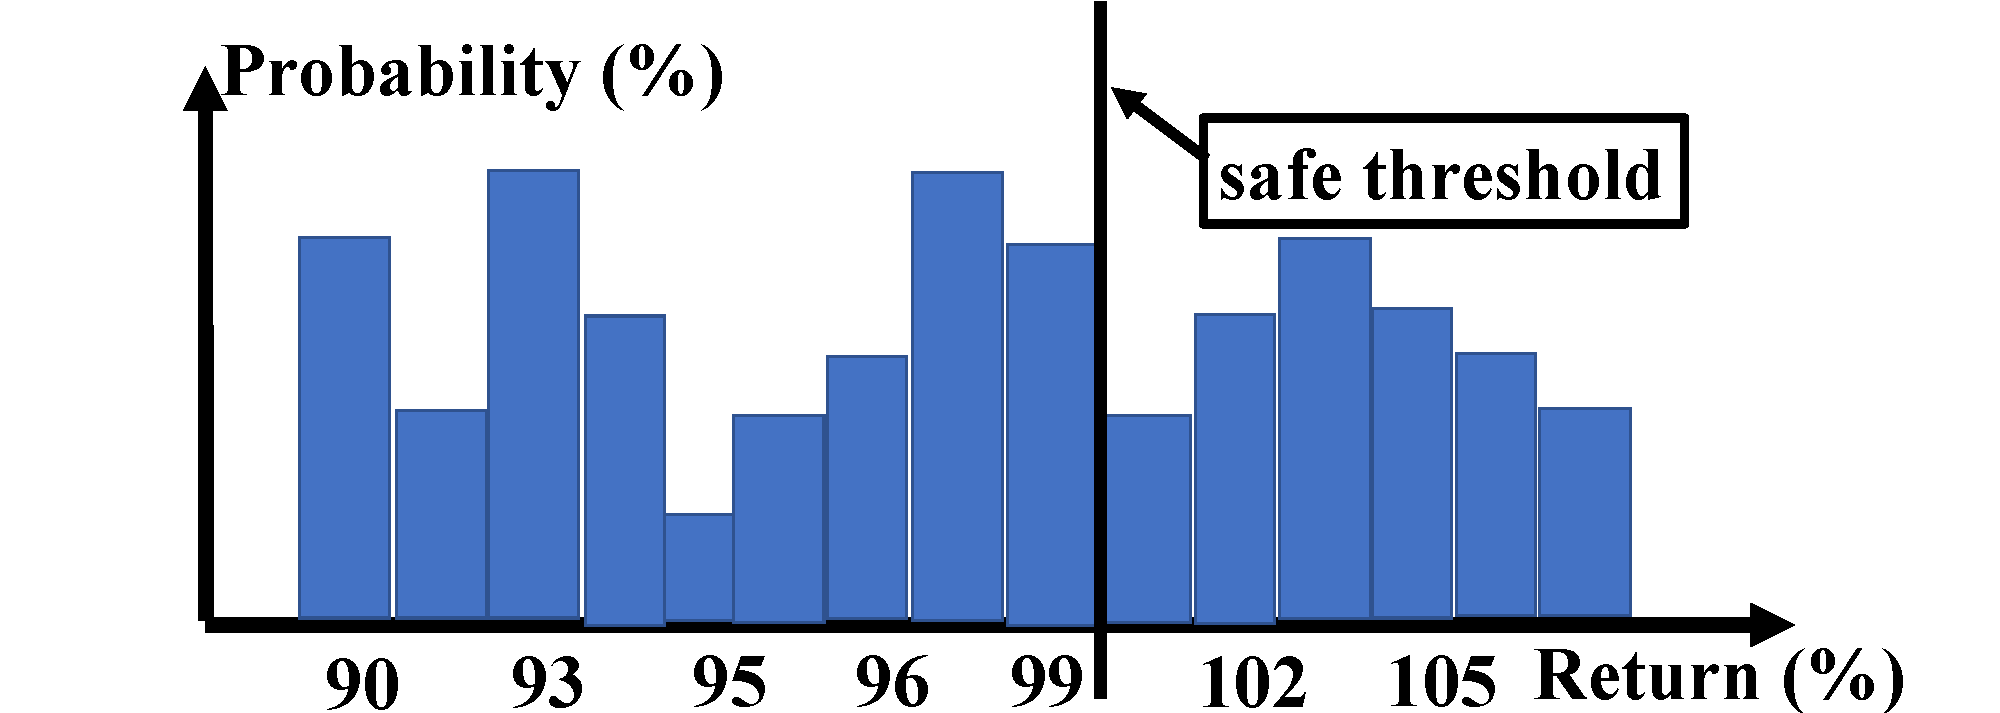
\includegraphics [width=0.9\columnwidth] {fig/return.pdf}
%\caption{Transfer return under different network states.}
%\label{Time-fig}
%\end{center}
%\end{figure}

% $S_j$ &\multicolumn{6}{|l}{Network service achieved availabitlity of $j$}\\
%\hline

%Besides whether the new arrival demand can be admitted, Algorithm \ref{greedy-1} also outputs pre-allocation results.


%Firstly, it sorts all the services j ∈ J in non-decreasing order according to the ratio of importance to efficient bandwidth demands, where the efficient bandwidth demands are derived as ∑k∈K d jk β j (Line 1).  It next sorts network scenarios and tunnels of each node pair (Line 2-3). For each service j ∈ J, the algorithm calls Algorithm 3 to check whether the remaining network capacity can satisfy its bandwidth-based availability (Line 7). If the network is unable to support its bandwidth-based availability and the current service is more profit than the total previous items (Line 8), the algorithm will try to recycle total resources and test that if allocating total network resources can support j (Line 10). If this is true, then algorithm will use the new allocation results (Line12-14). At last, for the remaining network resource, the algorithm will solve the following LP problem (Line 15):



\subsection{Traffic scheduling} \label{TE}

For each \textit{admitted} demand, the traffic scheduling determines bandwidth allocation over each tunnel every $T$ (e.g., 10 mins).
Traffic scheduling aims to satisfy each BA demand's availability target and we model the traffic scheduling as a linear programming.
%(2) To provide high availability, networks are over-provisioned,  and the traffic engineering should route requests with route all admitted requests with small induced network overload, so that more network resources could be used to accommodate future requests;
%(3) The algorithm should be fast enough to derive the routing solution.
%We begin with the constraints.
Firstly, the bandwidth allocation results $f_{d}^t$ for BA demand $d$ over tunnel $t \in T_{k}$ should be non-negative, i.e.,
\begin{equation}
f_{d}^t \ge 0, \quad\forall d \in D ,  k\in K,   t\in T_{k}.
\label{constraint-f2}
\end{equation}
Then total traffic through link $e$ should not be larger than its capacity $c_e$:

\begin{equation}
 \sum_{d \in D}\ \sum_{k\in K:t\in T_{k}}f_{d}^tu_t^e \le c_e, \quad \forall e \in E.
\label{constraint-e2}
\end{equation}

To provider high availability with minimum induced overload, we restrict each demand's total allocated bandwidth smaller than its real need, i.e., 


\begin{eqnarray} \label{Smaller}
 \sum_{t\in T_{k}} f_{d}^t \le \mathbf{b}^k_d, \quad  \forall d \in D_a, k \in K
\end{eqnarray}


$R_{dk}^{\bm{z}}$ is the ratio of total reserved bandwidth to demand through pair $k$ for BA demand $d$ under network scenario $\bm{z}$ and it is defined as:

 \begin{eqnarray} \label{R2}
R_{dk}^{\bm{z}}=\frac{\sum_{t\in T_{k}}f_{d}^tv_t^{\bm{z}} }{\mathbf{b}^k_d}, \quad \forall  d \in D, \bm{z}\in \bm{Z}, k \in K.
\end{eqnarray}

%Figure \ref{Time-fig} gives an illustration on resource allocation return.
%For a given bandwidth allocation vector, it plots the sorted return and the corresponding probability.
$R_{dk}^{\bm{z}}$ describes the allocation return under network scenario $\bm{z}$.
In reality, tunnel $t$ might be unavailable (i.e., $v_t^{\bm{z}} =0$), and if the total reserved bandwidth through all the available tunnels is larger than $\mathbf{b}^k_d, \forall k \in K$,  then bandwidth demand can still be satisfied and network scenario $\bm{z}$ can be regarded as \textit{qualified}, i.e., 
$R_{dk}^{\bm{z}} \ge 1, \forall k \in K$.
To guarantee the availability target of a demand, we should make its total probability of qualified scenario larger than availability target, i.e., 
$\sum_{\forall k: R_{dk}^{\bm{z}} \ge 1} p_{\bm{z}} \ge \beta_d, \forall d \in D_a$.
%This is a step function and we define the following potential function:
% 
%  \begin{eqnarray} \label{B3}
%\sum_{R_{dk}^{\bm{z}} \ge 1} p_{\bm{z}} \ge \beta_i, \forall d \in D_a
%\end{eqnarray}
%$R_{dk}^{\bm{z}}$ is the ratio of allocated bandwidth to  demand over node pair $k$ under network scenario $\bm{z}$.
Let $B_d^{\bm{z}}$ denote the lower bound of $R_{dk}^{\bm{z}}$ over the $k$ pairs for  $i$ under network scenario $\bm{z}$,  i.e.,

 \begin{eqnarray} \label{B2}
B_d^{\bm{z}} \le R_{dk}^{\bm{z}}, \quad  \forall  d \in D_a, \bm{z}\in \bm{Z}, k \in K
\end{eqnarray}

It is obvious  $B_d^{\bm{z}} \le 1$ and $B_d^{\bm{z}}=1$ presents scenario $\bm{z}$ is qualified, therefore, 
we can define $B_d^{\bm{z}}\times p_{\bm{z}}$  as the potential achieved availability of $i$ under network scenario  $\bm{z}$.
To satisfy diverse availability targets, the achieved availability should be larger than availability target, i.e., 
 
 \begin{eqnarray} \label{Achieved}
\sum_{\bm{z}\in \bm{Z}}B_d^{\bm{z}}\times p_{\bm{z}} \ge \beta_{d},  \quad {\forall d \in D_a}
\end{eqnarray}



We want to maximize the overall achieved availability of all admitted demands,  thus,  we can finally give the formulation of traffic engineering formulation: 



\begin{equation}
\small
\begin{aligned} \label{BATE-TE}
 &maximize  \sum_{i\in I_a} \sum_{\bm{z}\in \bm{Z}}B_d^{\bm{z}}\times p_{\bm{z}}\\
&\begin{array}{r@{\quad}r@{}l@{\quad}l}
s.t. (\ref{constraint-f2}), (\ref{constraint-e2}), (\ref{Smaller}), (\ref{R2}), (\ref{B2}), (\ref{Achieved})
%\begin{cases}
% \sum_{d \in D_a}\ \sum_{k\in K}\sum_{t\in T_{k}}f_{d}^tu_t^e \le c_e, &\text{$\forall e \in E $.}\\
%R_{dk}^{\bm{z}}=\frac{\sum_{t\in T_{k}}f_{d}^tv_t^{\bm{z}} }{\mathbf{b}^k_d} , &\text{$\forall  d \in D_a, \bm{z}\in \bm{Z},  k \in K$.}\\
%R_{dk}^{\bm{z}}>=B_d^{\bm{z}},&{\forall d \in D_a, \bm{z} \in Z, k\in K.} \\
%\sum_{\bm{z}\in \bm{Z}}B_d^{\bm{z}}\times p_{\bm{z}} \ge \beta_{\gamma_{i}},&{\forall d \in D_a} .\\
% \sum_{t\in T_{k}} f_{d}^t \le \mathbf{b}^k_d, &{  \forall d \in D_a, k \in K}.\\
%f_{d}^t \ge 0,&{\forall d \in D_a , \forall k\in K,\forall t\in T_{k}}.\\
%\end{cases}\\
\end{array}
\end{aligned}
\end{equation}

% \begin{figure}[t]
%\begin{center}
%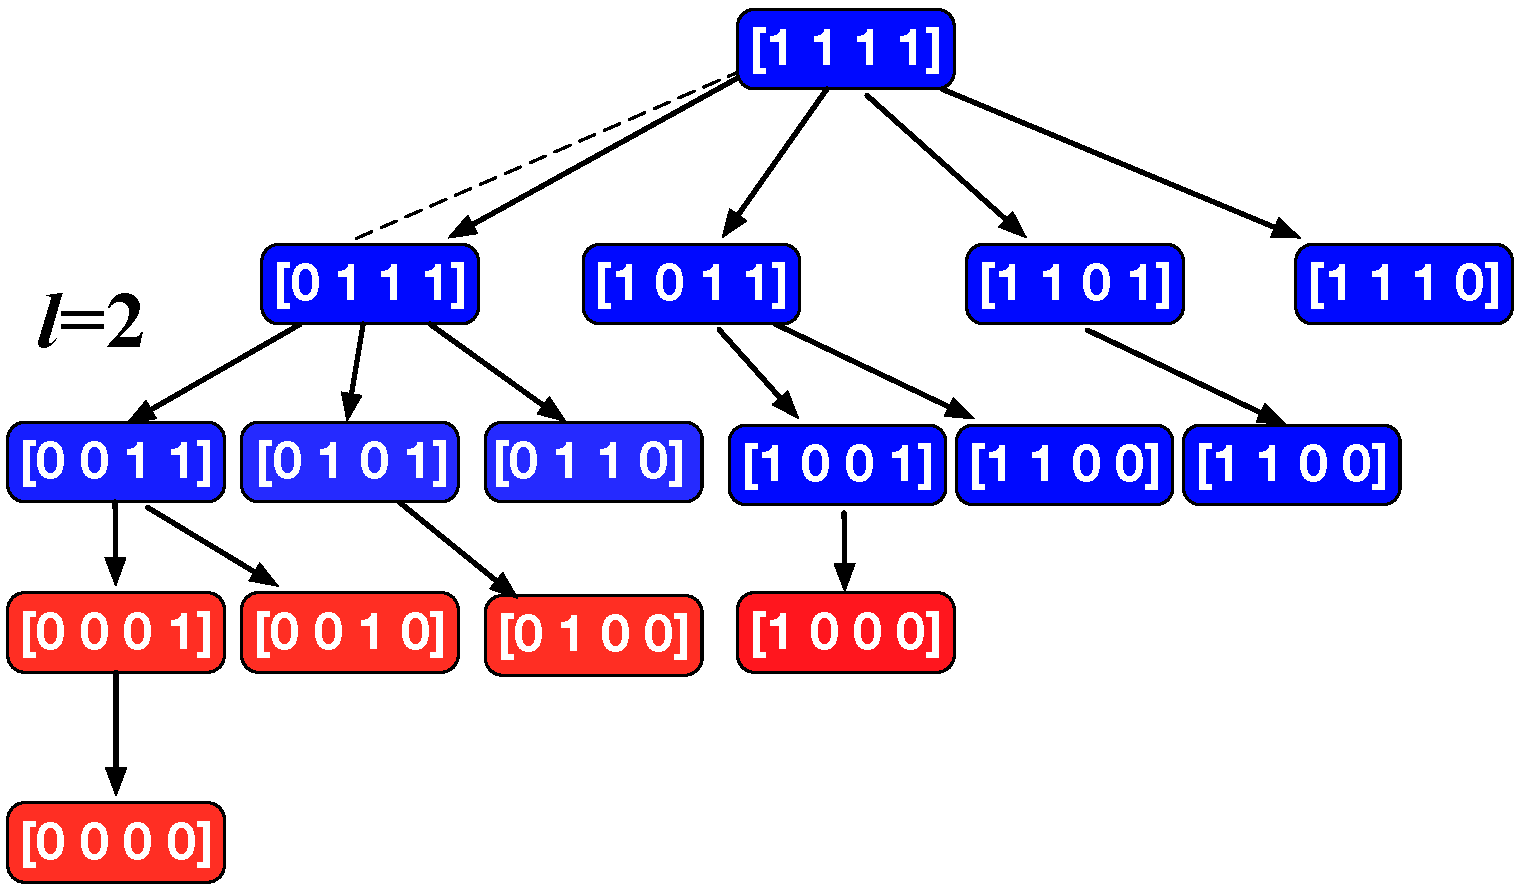
\includegraphics [width=0.8\columnwidth] {fig/pic.pdf}
%\caption{An example of concurrent failure number based pruning tree, where the $i$-th layer denotes concurrent $i$ link failures could happen. Network scenarios (red) located in layer 3, 4 are pruned in this example.}
%\label{pic-fig}
%\end{center}
%\end{figure}



We can see that although the traffic engineering module is LP problem, it considers each network scenario, which makes problem complexity increase exponentially with network size.
%For example, we consider a small inter-DC WAN which contains 3 links and  5 events.
%Each link has $2^5=32$ states and the network includes $32^3=32768$ states in total. 
%In reality, network scale is much larger and  the states volume will increase exponentially.
For instance, B4 \cite{B4}  topology has 12 nodes and 38 links, then there are $2^{38}-1$ network failure scenarios in total.
%The explosive network scenarios make it impossible to solve $\mathsf{BATE}$ problem.
Therefore,  an important question is  \textit{how to effectively reduce the size of  traffic engineering problem?} 


Previous literatures such as TEAVAR \cite{Teavar} advocate to prune scenarios which has smaller probability than a threshold, therefore, problem scale will reduce. 
This method is easy but the accuracy and efficiency tradeoff threshold is hard to decide.
A large threshold could significantly accelerate the algorithm since large amount of network scenarios are cut off, however, the accuracy might decrease.
Instead, we propose to cut off network failure scenarios in which \textit{concurrent link failure number} is larger than $l$.
We think this method is much more practical since most scenarios could hardly happen (e.g., more than two links fail simultaneously). 
Therefore, we can ignore these scenarios.
To provide an upper bound of the traffic engineering problem, we collapse all the pruned scenarios into a single scenario with probability equal to the sum of probabilities of the pruned scenarios and regard that scenario as an unsafe one.
%Figure \ref{pic-fig} depicts an example of a simple network with four links when $l=2$. 
%The root node denotes all
%links are available (i.e., $[1111]$). 
%The $i$-th layer denotes concurrent $i$ link failures could happen. 
%Network scenarios (red) located in layer 3, 4 are pruned (the root node is regarded as layer 0).
%\begin{equation}
%\small
%\begin{aligned} \label{BATE-TE}
% &maximize  \sum_{i\in I} \sum_{\bm{z}\in \bm{Z}}B_d^{\bm{z}}\times p_{\bm{z}}\\
%&\begin{array}{r@{\quad}r@{}l@{\quad}l}
%s.t.
%\begin{cases}
% \sum_{d \in D}\ \sum_{\forall k\in K: t\in T_{k}}f_{d}^tu_t^e \le c_e, &\text{$\forall e \in E $.}\\
%R_{dk}^{\bm{z}}=\frac{\sum_{k\in K}\sum_{t\in T_{k}}f_{d}^tv_t^{\bm{z}} }{\mathbf{b}^k_d} , &\text{$\forall  d \in D_a, \bm{z}\in \bm{Z},  k \in K$.}\\
%R_{dk}^{\bm{z}}>=B_d^{\bm{z}},&{\forall d \in D_a, \bm{z} \in Z, k\in K.} \\
%\sum_{\bm{z}\in \bm{Z}}B_d^{\bm{z}}\times p_{\bm{z}} \ge \beta_{\gamma_{i}},&{\forall d \in D_a} .\\
% \sum_{t\in T_{k}} f_{d}^t \le \mathbf{b}^k_d, &{  \forall d \in D_a, k \in K}.\\
%f_{d}^t \ge 0,&{\forall d \in D_a , \forall k\in K: t\in T_{k}}.\\
%\end{cases}\\
%\end{array}
%\end{aligned}
%\end{equation}

%When all demands have the same availability targets , similar to TEAVAR \cite{Teavar},  $\mathsf{BATE}$ is also able to strike a good balance between network utilization and availability.
%Compared with TEAVAR,  $\mathsf{BATE}$ has the following two advantages:
%Firstly, $\mathsf{BATE}$  is not as aggressive as TEAVAR. 
%Flows can gain more bandwidth than their needs under TEAVAR \cite{Teavar}, while they can't exceed demands under  $\mathsf{BATE}$.
%Therefore, a more reasonable balance between network utilization and availability can be achieved when network is much over-provisioned.
%Secondly, when network is under-provisioned, $\mathsf{BATE}$ can make demands with stringent availability requirements pass links with high reliability, therefore, their availability targets can be guaranteed, but TEAVAR is unable differentiate demands from tenants.
%Compared with TEAVAR \cite{Teavar}, our traffic engineering has the following two advantages:
%(1)




\subsection{Failure recovery} \label{backup}
In $\mathsf{BATE}$,  traffic can also be redistributed across the surviving tunnels via rerouting when any tunnel becomes unavailable.
%Previous tunnel-based traffic engineering schemes (such as FFC) keep link utilization low to prevent congestion when there are failures.
%Different from them, links have less vacant capacity under $\mathsf{BATE}$, therefore, when there are failures, re-routing might cause congestion.
%When a link $e'$ fails, all tunnels through this link  fails.
In reality, service providers have to derive refunding credits for violating availability targets (see $\S$\ref{background}).
$\mathsf{BATE}$ proactively considers failure scenarios and pre-computes backup allocation to maximize total revenue, and the surviving tunnels can be used immediately to support tenants.
%Each tunnel belongs to one flow pair.
%We can divide all node pairs into two groups, i.e.,  victim node pairs and normal node pairs, which is similar to \cite{sentinel}.
%Let $H$ denote all the victim node pairs when link $e'$ fails.
%Assume link $e'$ will fail, the normal tunnel set is $Q_{k}$ and the backup tunnel set is $Q'_{k}$.
%In reality, the backup tunnel set can be pre-computed by the network operators beforehand.
For example, Figure \ref{recovery} shows two services are from DC1 to DC4 and both of them need bandwidth demand of 2.
Link capacity is 1 everywhere.
Figure \ref{recovery}(a) shows the original traffic engineering allocation and it is used when no failures happen.
%if we assume the link between DC2 and DC4 is down, then DC1$\to$DC4 is victim node pair and DC1$\to$ DC2 is normal pair. 
%the backup tunnel set $Q'$=\{DC1$\to$DC2$\to$DC3$\to$DC4\} and normal tunnel set is 
%$Q$ =\{DC1$\to$DC3$\to$DC4\} for the victim node pair DC1$\to$DC4.
%Let $M_e$ denote the used bandwidth of link $e$ by normal node pairs,
Figure \ref{recovery}(b) depicts the backup allocation result when we assume the link between DC2 and DC4 is down, and the result will be put into practice when link DC2 $\to$ DC4 failure is detected.
Network scenario number is huge for large-scale network and we assume that at any time, only one link in the network could fail. 
If we assume network scenario $ \bm{z}$ could happen, and let 
%$f^{\bm{z}}_{ikt}$ denote bandwidth of $i$ over tunnel $t\in T^{ \bm{z}}_k$, where 
$T^ { \bm{z}}_k$ denote the surviving tunnel set under scenario $ \bm{z}$ and the bandwidth allocated for demand $d$ over tunnel $t$ should be non-negative, i.e.,
\begin{equation}
f^{t}_{d} \ge 0, \quad\forall d \in D ,  k\in K : t\in T^{\bm{z}}_k.
\label{constraint-f3}
\end{equation}


Let $A_e^{ \bm{z}}$ denote whether link $e$ is available under scenario $ \bm{z}$.
The total bandwidth should be smaller than capacity for each available link, i.e.,  

\begin{figure}[t]
\centering
\subfigure[Original TE allocation]{
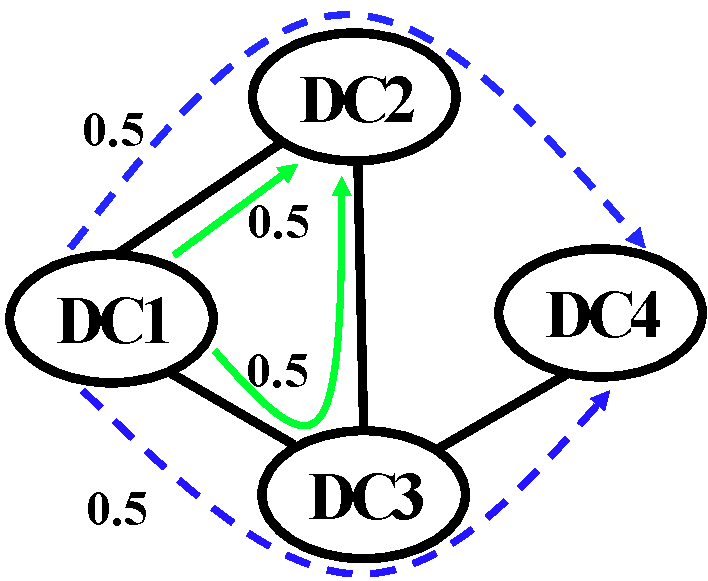
\includegraphics[width=0.23\textwidth]{fig/recovery-1.pdf}}
\subfigure[Backup allocation]{
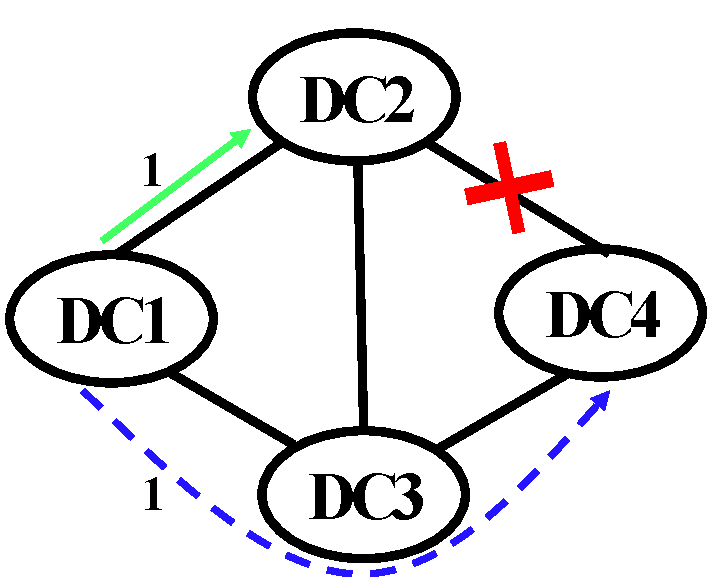
\includegraphics[width=0.23\textwidth]{fig/recovery-2.pdf}}
\caption{There are two services from DC1 to DC4 and link capacity is 1 everywhere. (a) shows the original TE allocation. (b) shows the backup allocation result when assuming link DC2 $\to$ DC4 is broken.  }
\label{recovery}
\end{figure}
%\begin{equation}
%\small
%\begin{aligned} \label{BATE-recovery}
% &maximize  \sum_{i\in I_a} \sum_{\bm{z}\in \bm{Z}}B_d^{\bm{z}}\times p_{\bm{z}}\\
%&\begin{array}{r@{\quad}r@{}l@{\quad}l}
%s.t.
%\begin{cases}
%\sum_{i\in I_a}\sum_{k\in K}\sum_{t\in Q_{h}} f'_{ikt}u_t^e+ \sum_{i\in I_a}\sum_{k\in K}\sum_{t'\in Q_{h}} f''_{ikt'}L_{t'e} \le c_e, &\text{$\forall e \in E \setminus e' $.}\\
%R_{dk}^{\bm{z}}=\frac{\sum_{k\in K}\sum_{t\in T_{k}}f_{d}^tv_t^{\bm{z}} }{\mathbf{b}^k_d} , &\text{$\forall  d \in D_a, \bm{z}\in \bm{Z},  k \in K$.}\\
%R_{dk}^{\bm{z}}>=B_d^{\bm{z}},&{\forall d \in D_a, \bm{z} \in Z, k\in K.} \\
%\sum_{\bm{z}\in \bm{Z}}B_d^{\bm{z}}\times p_{\bm{z}} \ge \beta_{\gamma_{i}},&{\forall d \in D_a} .\\
% \sum_{t\in T_{k}} f_{d}^t \le \mathbf{b}^k_d, &{  \forall d \in D_a, k \in K}.\\
%f_{d}^t \ge 0,&{\forall d \in D_a , \forall k\in K,\forall t\in T_{k}}.\\
%\end{cases}\\
%\end{array}
%\end{aligned}
%\end{equation}



\begin{small}
\begin{eqnarray} \label{B-constraint}
\sum_{d\in D_a}\sum_{k\in K:t\in T^{ \bm{z}}_k} f^{t}_{d}u_t^e \le c_e \times A_e^{ \bm{z}}
\end{eqnarray}
\end{small}

The revenue return for $i$ over node pair $k$ can be described:
\begin{small}
\begin{eqnarray} \label{B-return}
R_{dk}=\frac{\sum_{t\in T^{ \bm{z}}_k} f^{t}_{d}}{\mathbf{b}^k_d}, \forall  d \in D_a,  k \in K
\end{eqnarray}
\end{small}


If the allocated bandwidth  of BA demand $d$ between each node pair is larger than its need (i.e., $R_{dk} \ge 1, \forall d \in  D_a$), the profit unit is 1, 
%If it is between $\beta_j^{k}$ and $\beta_j^{k+1}$, then the profit is $\alpha_j^k$, where $1>\alpha_j^1>\alpha_j^2>...>\alpha_j^k$.
otherwise, there is a penalty, which can be derived from SLA and we use $\mu_{d}$ to denote its penalty.
Then, the profit of $d$ is:



\begin{equation}
\forall  d \in D_a : h_d=
\begin{cases}
1 &\text{$\forall k \in K: R_{dk} \ge 1 $}\\
\mu_{d} &\text{Otherwise}
\end{cases}
\label{availability222}
\end{equation}

It is a step function and we can change it to the following linear format and we can also change it into a linear format:

\begin{equation}
\begin{cases}
h_d=y_d+\mu_{d}*(1-y_d),&{\forall d \in D_a.} \\
R_{dk} < M*y_d+1-y_d,&{\forall d \in D_a,  k\in K.} \\
R_{dk} >= y_d,&{\forall d \in D_a,  k\in K.} \\
y_d \in\{0,1\},&{\forall d \in D_a.} \\
\end{cases}
\label{A-SSS2}
\end{equation}

Where $M$ is a big integer that is at least larger than the upper bound of $R_{dk}$.
Let $w_d$ denote the profit of demand $d$ when its availability target can be satisfied.
The goal of failure recovery is to maximize profits of all the admitted demands, and we can give the problem formulation finally:

\begin{equation}
\small
\begin{aligned} \label{BATE-recovery}
 &maximize  \sum_{d\in D_a} w_d\times h_d\\
&\begin{array}{r@{\quad}r@{}l@{\quad}l}
s.t.  (\ref{constraint-f3}), (\ref{B-constraint}), (\ref{B-return}), (\ref{A-SSS2})
\end{array}
\end{aligned}
\end{equation}


The auxiliary output variables $y_d$ are chosen from \{0,1\},  so that the  failure recovery problem is a 0-1 Mixed-integer linear programming.

\begin{lemma}\label{NP-hard}
The failure recovery problem is NP-hard.
\end{lemma}
The detailed proof can be found in Appendix \ref{appendix1}.



As the failure recovery problem is NP-hard and one important question is \textit{can we develop an efficient algorithm to solve it in polynomial time?} 
%For the second challenge, although the powerful mathematical optimization solver such as Gurobi \cite{gurobi} can derive the solution, it might be too slow to converge before next TE scheduling epoch.
In this case,  we propose a greedy algorithm to attain an approximate solution whose pseudocode is shown in Appendix \ref{B}.
The key idea of the greedy algorithm is to give priority to demands in non-decreasing order by the ratio of profit to its efficient bandwidth demands.
\textit{We also prove the approximation of the greedy algorithm is 2  in Appendix \ref{B}}. 
%The greedy algorithm can solve $\mathsf{BATE}$  problem in  $O(|J||Z||T_k||E|)$ time.
%We further explore the accuracy of greedy algorithm in Section \ref{evaluation}.



\section{system implementation} \label{system}
%In this section, we show the design and some implementation details of $\mathsf{BATE}$ prototype.
%In this section, we show the design of $\mathsf{BATE}$ (Traffic Engineering for Diverse Availability Targets) system, which is able to provide high bandwidth-based availability to services.
%$\mathsf{BATE}$ system tries to achieve the following objectives:
We have implemented $\mathsf{BATE}$ on the Linux platform. Figure \ref{pic-overview} shows the whole system architecture, which contains one controller, multiple brokers (one for each DC) and multiple clients (one for each host). The controller is responsible for most decision work of $\mathsf{BATE}$, including admission control, traffic scheduling, and failure recovery, while the brokers and clients are responsible for bandwidth enforcement.
It works as follows:
When a user submits a demand to the controller, the admission control module determines whether the demand can be admitted or not (see $\S$ \ref{admission_control}).
If the demand is admitted, this module will also allocate its demanded bandwidth on appropriate paths for the first time, and notify the brokers for enforcement. The online scheduler module performs traffic scheduling (see $\S$ \ref{TE}) periodically  (e.g., every 10 minutes) to further optimize the availability expectation of all active demands. In addition, 
for potential link failures, it also pre-computes backup allocation strategies that will be activated if any link failure indeed happens (see $\S$ \ref{backup}). These central decisions are distributed to the brokers for bandwidth enforcement. The brokers in each DC monitor link status and bandwidth consumption, report these statistics to the central controller, and ask the clients to implement appropriate rate limit on end hosts. 

%The controller performs traffic engineering algorithm every $T_a$ (e.g., 10) minutes to derive the bandwidth allocation results.

% then it limits rate according to the responses from its data center broker.


\textbf{Controller} is the brain of the whole system. It is responsible for allocating WAN level bandwidth, and orchestrates all activities with a global view. The four main components in Controller are as follows.
(1) Offline Routing.
This module maintains the WAN level network topology, and computes TE tunnels between each node pair
 (i.e., $T_k,\forall \text{s-d pair} k \in K$), using certain routing algorithms (oblivious routing \cite{SMORE}, k-shortest path \cite{swan}, etc.). 
 %When topology changes (e.g., remove a node) are reported to controller, the TE Routing module will perform routing algorithm (oblivious routing \cite{SMORE}, k-shortest path \cite{swan}, etc.) to derive all the possible tunnels between each node pair (i.e., $T_k,\forall k \in K$) offline.
These tunnels are used by the admission control module and the online scheduler module as input variables;
(2) Admission Control.
When a BA demand is submitted, this module uses the admission control algorithm (see $\S$ \ref{admission_control}) to reject it, or accept it and allocate bandwith over the tunnels in nearly real-time.
The results are sent to the corresponding brokers.
(3) Online Scheduler. 
Periodically, This module performs traffic scheduling (see $\S$ \ref{TE}) according to the bandwidth availability demands submitted by users, so that the availability can be optimized in an expected manner. 
It also pre-computes backup allocation (see $\S$ \ref{backup}) for some potential link failures.
For each user demand, the normal bandwidth and backup bandwidth allocated over each tunnel (i.e., $f_i^t$) are then sent to the corresponding brokers. 
In addition, our system also supports several other TE algorithms including SWAN \cite{swan}, FFC \cite{FFC} and TEAVAR \cite{Teavar}.
(4) Communication Channel.
This module is responsible for communication with brokers, where we use long-lived TCP connections to avoid unnecessary delay. 
In addition, controller failures can be remedied by using multiple replications, 
where the master controller is elected by the Paxos \cite{lamport1998the} algorithm.
%To handle controller failure, the controller also replicate controllers and places them in different data centers, then Paxos \cite{lamport1998the} is used to elect one controller as the master.

\begin{figure}
\begin{center}
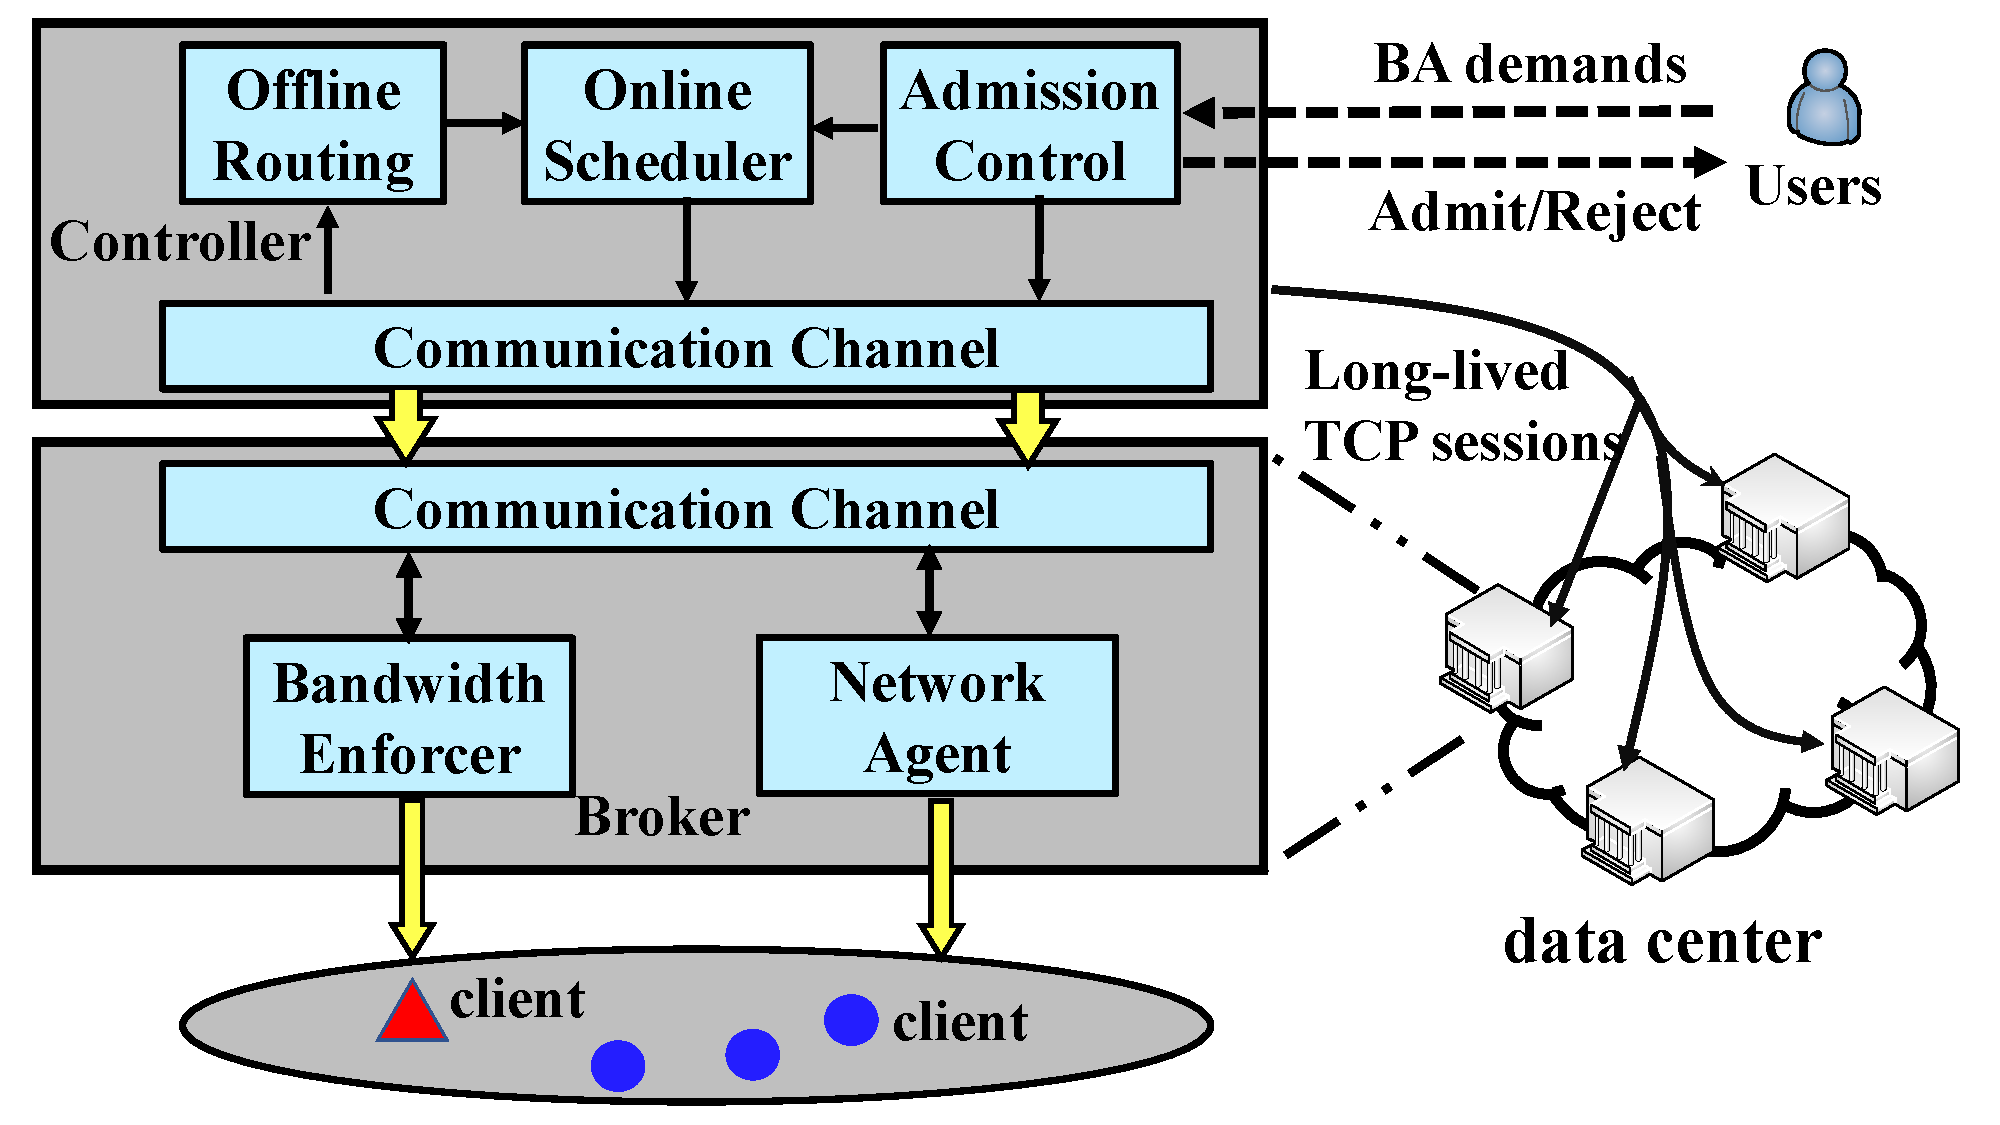
\includegraphics [width=0.9\columnwidth] {fig/inter-DC-WAN-V3.pdf}
\caption{System architecture of $\mathsf{BATE}$.}
\label{pic-overview}
\end{center}
\end{figure}

\textbf{Broker} takes care of the data center it resides in. It consists of three modules:
%(1) Demand  Aggregator.
%After receiving demands from hosts, brokers will aggregate them according to service over each node pair (i.e., $d_{jk}$).
%They are sent to controller along with the availability targets of each service (i.e., $\beta_j$);
%%The necessary information includes the application identifier, source address, destination address and expected bandwidth demand.
%Demand Collector gathers traffic demands and aggregates them on the basis of  flow identifiers (i.e., $ < AppID,Src,Dst >$);
%(2) \textit{Demand Predictior}.
%In $\mathsf{Dionysus}$ framework, resources should be able to be dynamic allocated according to the demands of applications.
%However, future application bandwidth demands can't be known beforehand, which makes it hard to adjust in real-time.
%The broker keeps the empirical demands collected by Demand Collector.
%With these history data, 
%Demand Predictior will predict the future bandwidth demands with data-driven algorithms such as ARIMA\cite{ARMA}, reinforcement learning \cite{Pensieve}; 
(1) Bandwidth Enforcer.
It receives the bandwidth allocation results (i.e., $f_i^t$) from controller, sends them to the corresponding hosts, and limits the actual traffic rate in each tunnel in case something is wrong on the end hosts;
(2) Network Agent.
We use commodity SDN switches at data center edges to connect DCs into an Inter-DC WAN.
The network agent runs in a SDN controller (we use floodlight \cite{floodlight}), 
and uses the OpenFlow \cite{openflow} protocol to installs and updates forwarding rules 
on the switches in the same DC. 
To reduce rule complexity, our system uses a label-based forwarding scheme, 
where the first 12 bits of a VxLAN ID represent different demands, 
and the last 12 bits represent different tunnels.
Therefore, 4096 demands and 4096 tunnels can be supported simultaneously, 
which can be further expanded if necessary. 
In this way, a flow (i.e., traffic corresponding to a BA demand) is marked with a label at the ingress switch, and the succeeding switches use this label for forwarding.
Group tables in the switch pipelines are used for flow splitting (i.e., traffic corresponding to a BA demand 
can be split into multiple sub-flows and transmitted in multiple tunnels).
%Flow table just maps the packet based on the destination and the group tables consist of bandwidth weight for each label.
Besides, the network agent also tracks the network topology, reports any change or failure to the central Controller module, and monitors the actual traffic rate. 
(3) Communication Channel.
This component is responsible for communication with the central Controller.
%In reality, many switches are able to detect link failure  \cite{FDT,olfd}.
%Brokers exploit this and send the failure information to controller after the edge switches detect link failures.

\textbf{Client} sits on each host to carry out rate limiting. 
%A shim in the host OS estimates its demand to each remote DC for the next $T_b$ minutes 
%and asks the broker for an allocation.
%Each client has a RPC daemon that submits its SLA to its DC broker every  $T_b$ (e.g., 1) minutes.
It consists of a daemon and a kernel module. The former recieves bandwidth allocation results from the site broker, while the latter sits between the TCP/IP stack and the Linux Traffic Control (TC) module to control outbound traffic rate. 

\iffalse
$\mathsf{BATE}$ system adopts OpenFlow\cite{openflow}  to install and update forwarding rules.
To reduce forwarding complexity, our prototype uses label-based forwarding.
%Traditionally,  VLAN header is tagged on the ingress switches and VLAN ID is often used to differentiate tunnels \cite{swan}.
%We abandon this as VLAN ID only contains 12 bits, which is insufficient to present bandwidth demand between each DC pair.
%Instead, 
We adopt VxLAN ID which contains 24 bits, where the first 12 bits to present demands and the remaining 12 bits are used to distinguish tunnels between each node.
Therefore, $2^{12}=4096$ tenants' demands and $2^{12}=4096$ tunnels can be supported simultaneously.
Flows are marked with a label at the ingress switch and the remaining switches can just read the labels and forward the packets.
To implement unequal bandwidth splitting, our prototype uses group table in its OpenFlow pipeline.
Flow table just maps the packet based on the destination and the group tables consist of bandwidth weight for each label.
\fi


%In reality, service providers often use a piecewise function to derive refunding credits for violating availability targets (see $\S$\ref{background}) and we can modify profit function to model this.
%Let $\{1,\beta_j^1,\beta_j^2....\}$ present the availability target list of service $j$.
%The corresponding profit list can be denoted as $\{1,\alpha_j^1,\alpha_j^2...\}$.
%If the achieved availability (i.e., $S_j$) is larger than the highest desired availability target (i.e., $\beta_j^1$), the profit is 1.
%If it is between $\beta_j^{i}$ and $\beta_j^{i+1}$, the profit is $\alpha_j^i$.
%Otherwise, it is a non-decreasing function  of $f_{jtk}$.
%Finally, the profit function can be formulated as:
%
%
%\begin{equation}
%\forall  j \in J : g_j=
%\begin{cases}
%1 &\text{$1>S_j \ge \beta_j^1$}\\
%\alpha_j^1 &\text{$\beta_j^1>S_j \ge \beta_j^2$}\\
%... &\text{$...$}\\
%\mu(f_{jtk})  &\text{$\beta_j^x>S_j \ge0$}
%\end{cases}
%\label{availability}
%\end{equation}
%
%Table \ref{target} shows how to explicitly model the availability targets of services under $\mathsf{BATE}$.
%For example, the profit for Microsoft Azure Traffic Manager service \cite{azure} shown in the first line of Table \ref{target}, can be modeled as:
%\begin{equation}
%g=
%\begin{cases}
%1 &\text{$1>S \ge 99.99\%$}\\
%0.9 &\text{$99.99\%>S \ge 99\%$}\\
%0.75 &\text{$99\%>S \ge0$}
%\end{cases}
%\label{availability222}
%\end{equation}


 \begin{figure}
\begin{center}
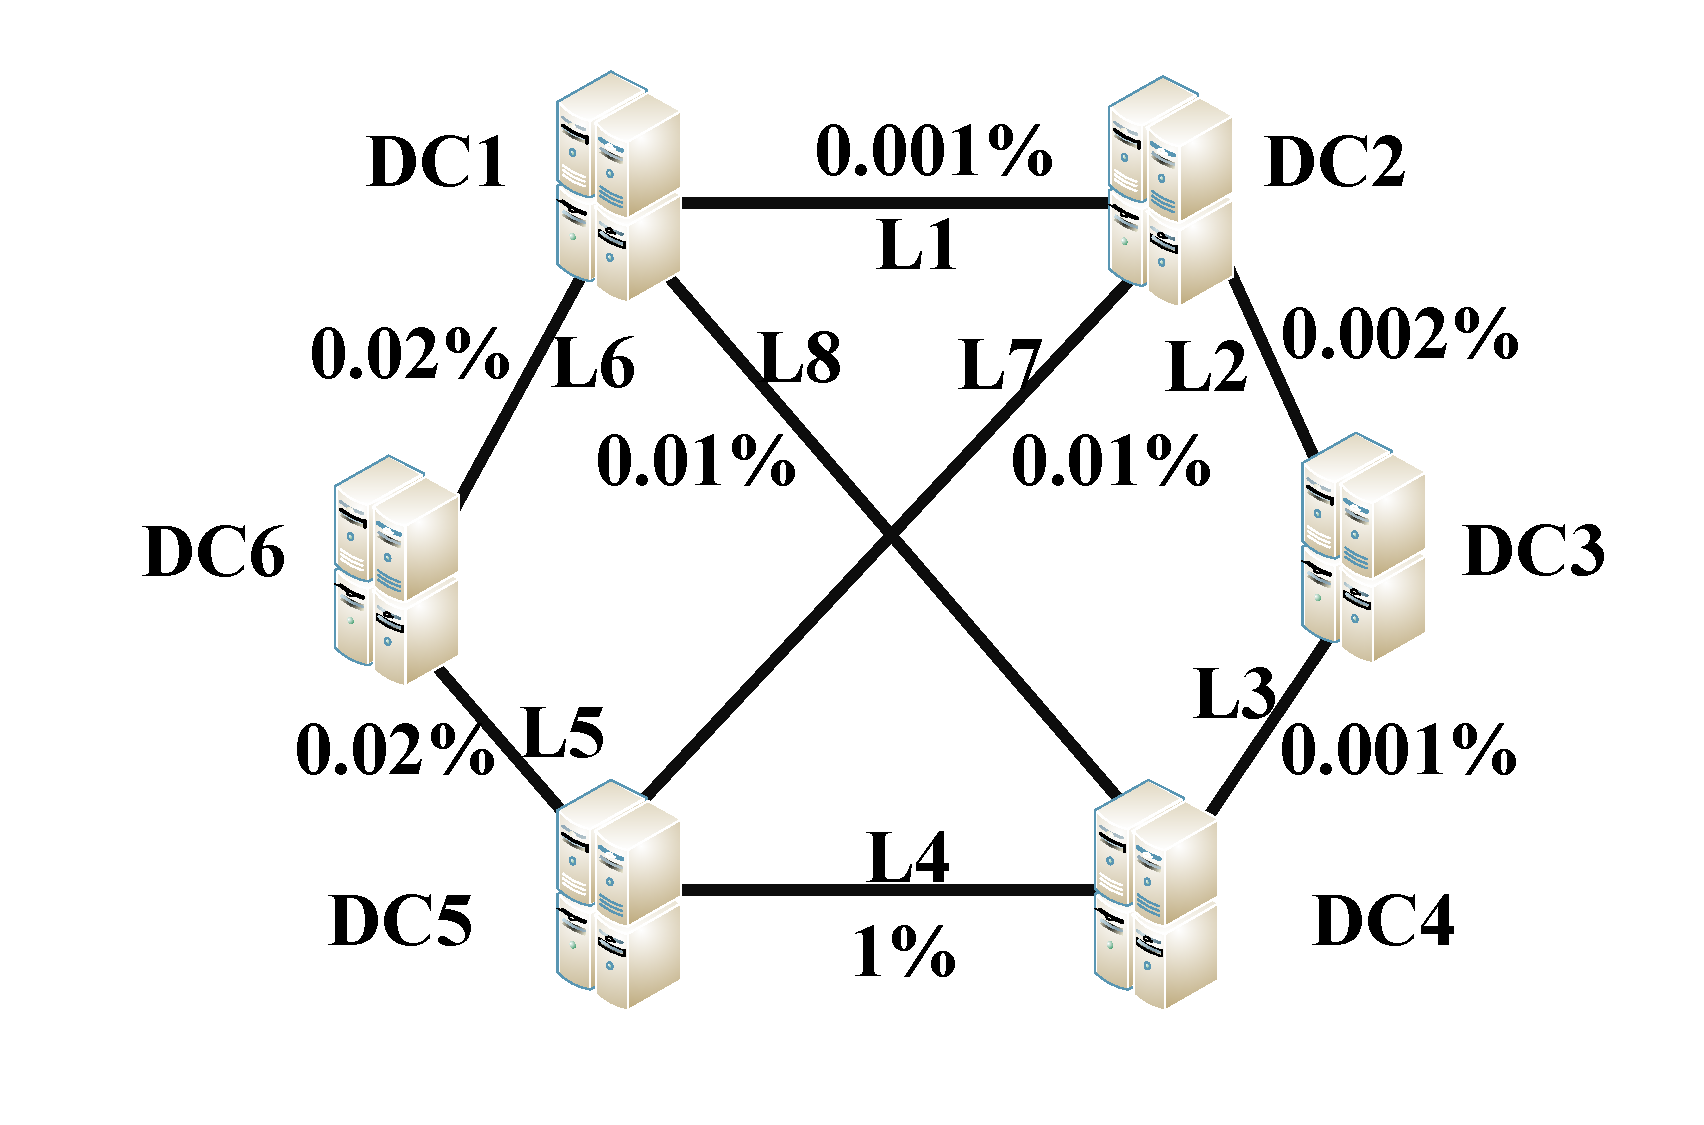
\includegraphics [width=0.8\columnwidth] {fig/testbed.pdf}
\caption{Testbed topology. Each link has the same capacity 1Gbps but  different failure probability.}
\label{testbed}
\end{center}
\end{figure}

\begin{figure*}
\centering
\subfigure[Admission control]{
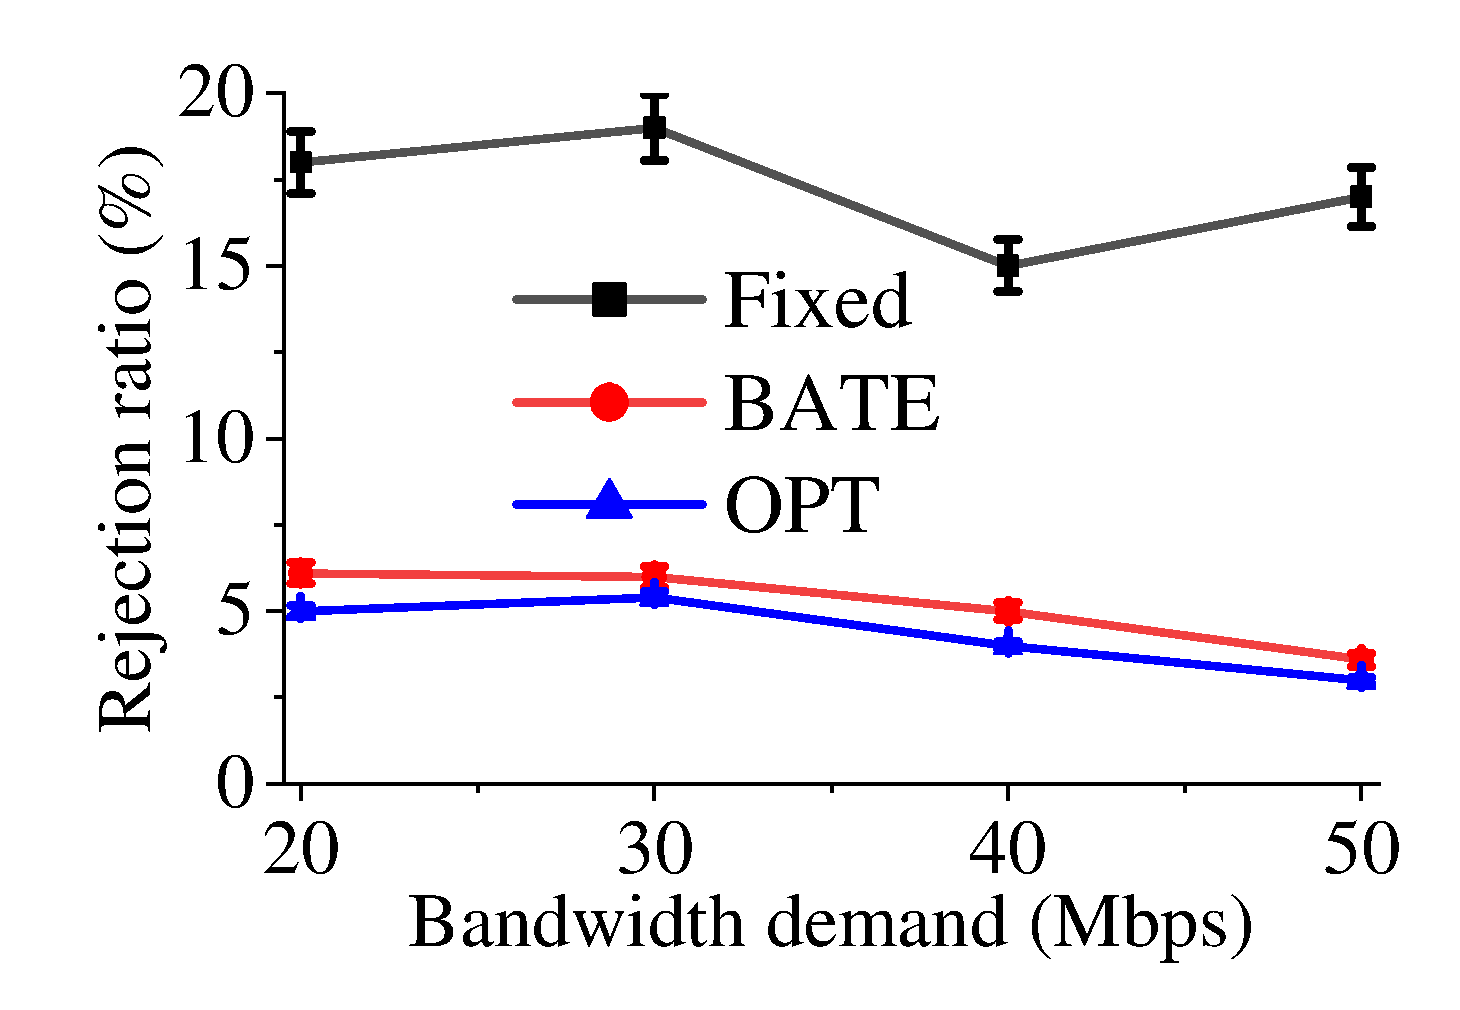
\includegraphics[width=0.24\textwidth]{fig/evaluation/testbed-admit.pdf}}
\subfigure[Measured and demand ratio]{
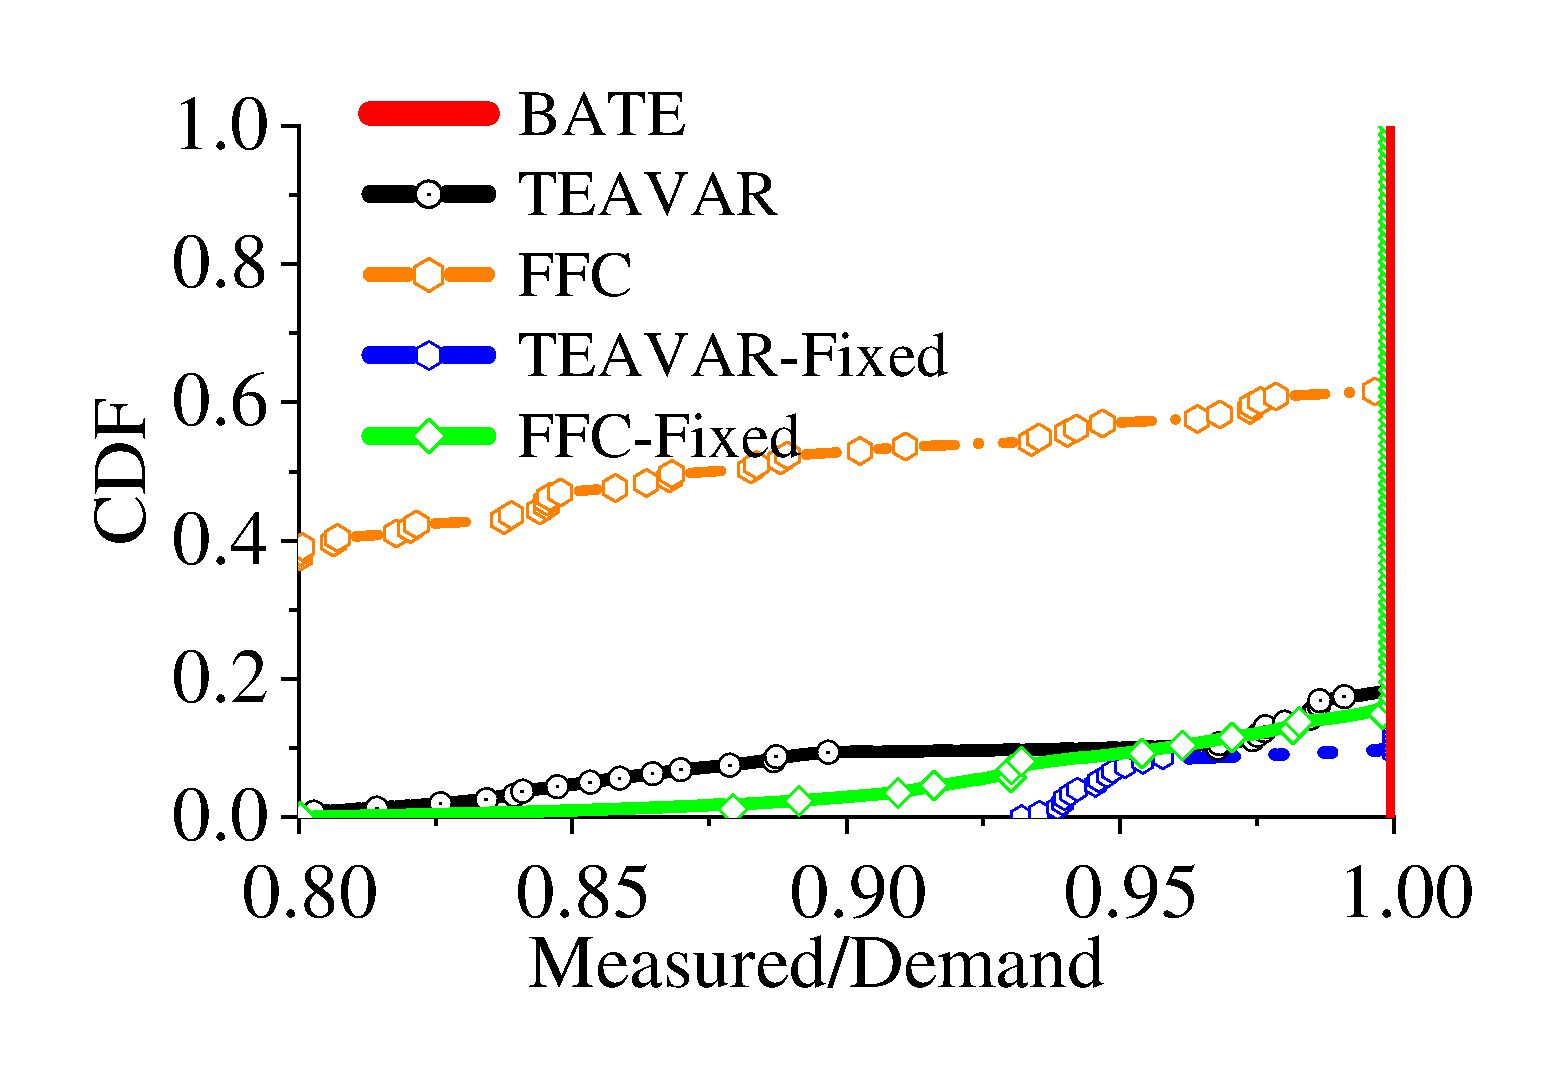
\includegraphics[width=0.24\textwidth]{fig/evaluation/testbed-public-2.pdf}}
\subfigure[Monetary gain after failures]{
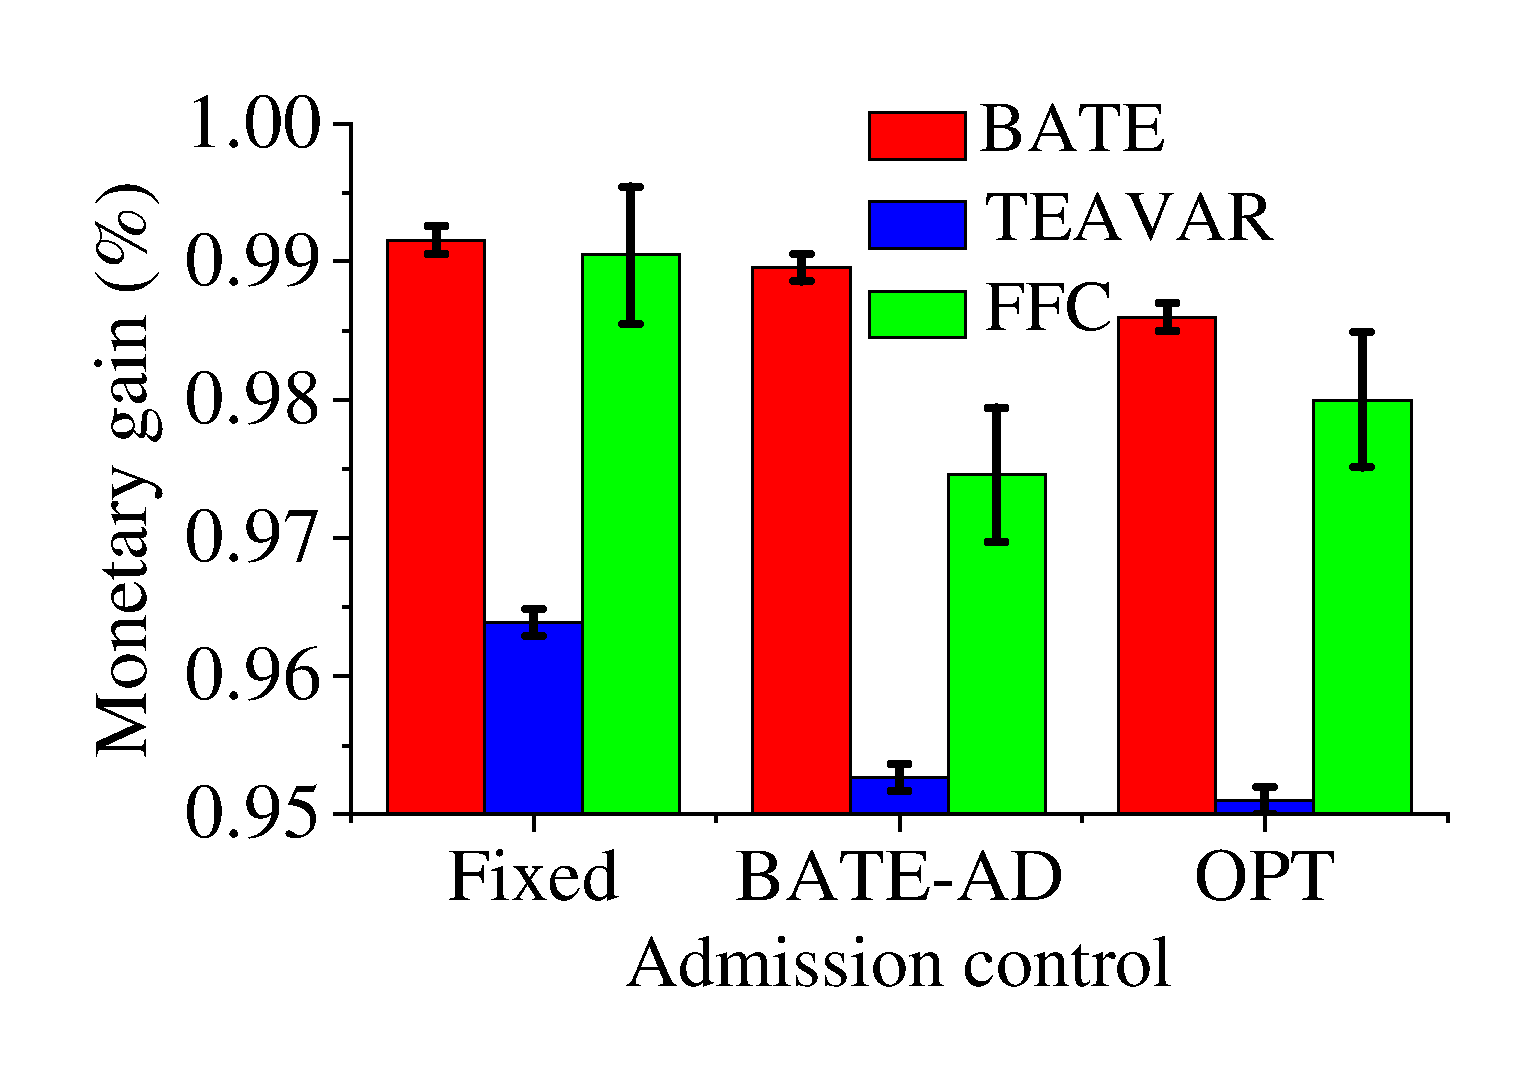
\includegraphics[width=0.24\textwidth]{fig/evaluation/test-bed-profit.pdf}}
\subfigure[Data loss ratio]{
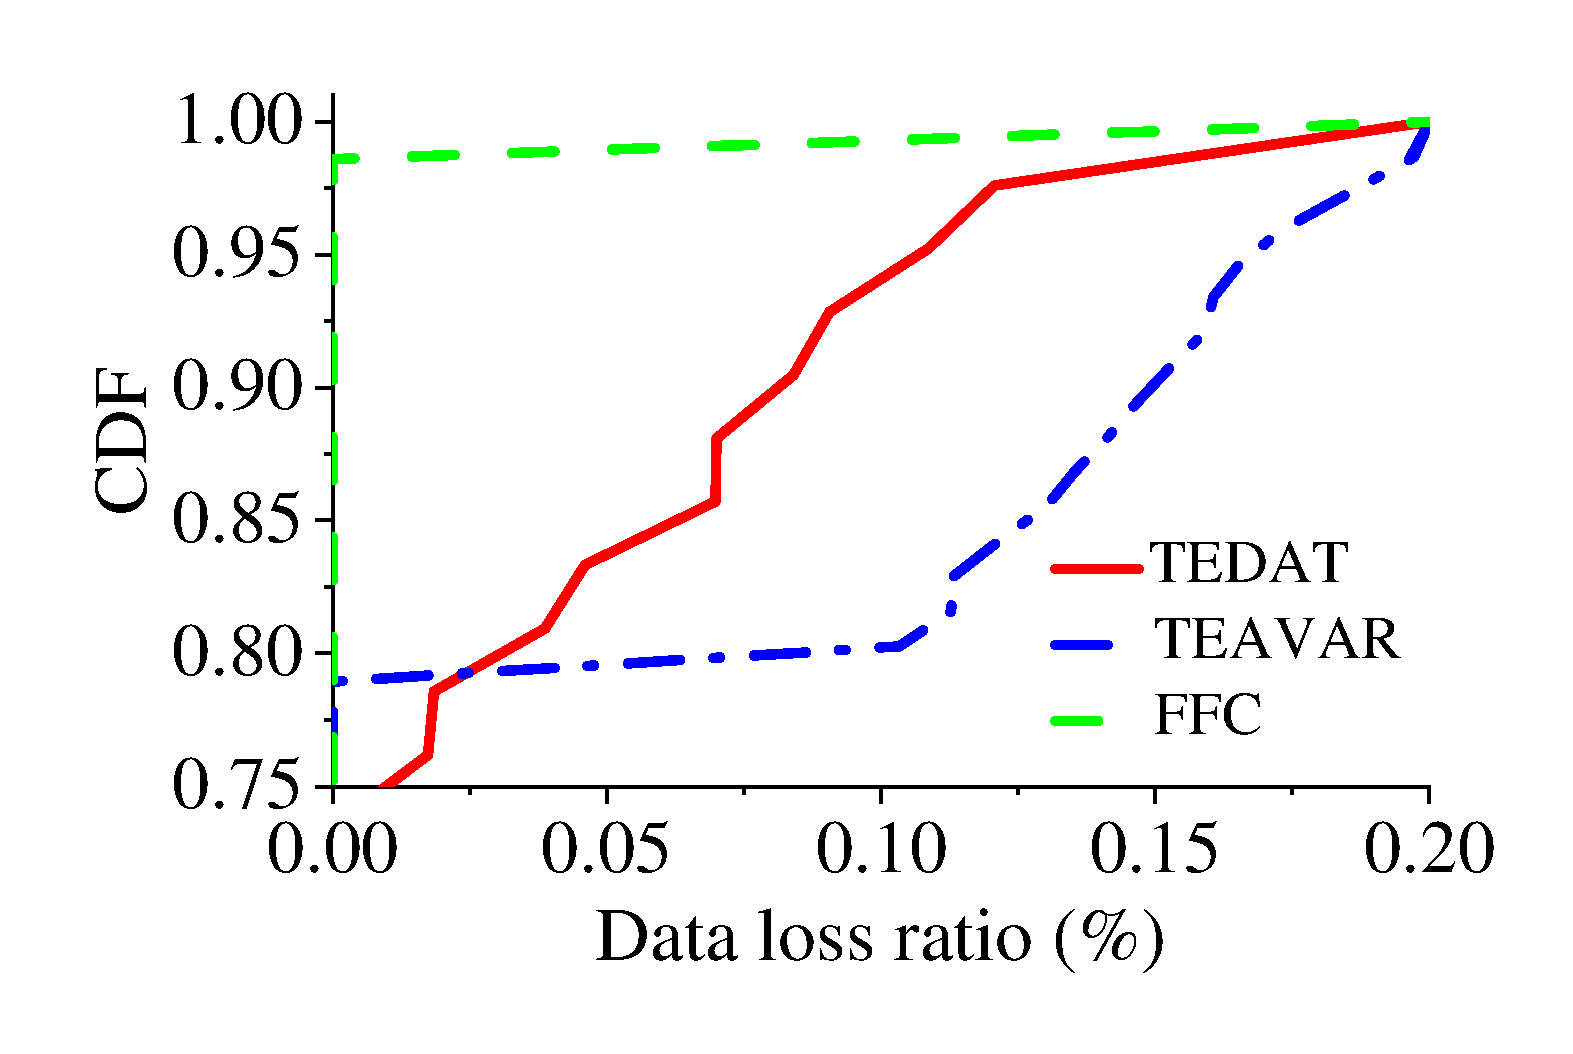
\includegraphics[width=0.24\textwidth]{fig/evaluation/testbed-data-loss-2.pdf}}
\caption{A public cloud example: tenants' demands arrive obeying poisson process and the duration of demands are with exponential distribution.}
\label{e2}
\end{figure*}


%The average error of traffic scheduling is within 8\% and the profit loss of greedy algorithm is less than 10\%. 

% \begin{itemize}
%  \item \textbf{What is the benefit of  $\mathsf{BATE}$ ?}
%  In $\S$ \ref{testbedresults}, we show $\mathsf{BATE}$ proactively considers link failure probability as well as the diverse demands of services proactively and it increases the percentage of services that satisfy their availability SLAs by up to 40\%. 
%  \item \textbf{How does $\mathsf{BATE}$ compare with the state-of-the-art traffic engineering TE schemes?} In $\S$ \ref{scales}, we show the consistent performance of  $\mathsf{BATE}$ under various topologies and traffic. $\mathsf{BATE}$ performs  up to 30\%, 40\%, 50\%, 75\% better than TEAVAR\cite{Teavar}, SMORE\cite{SMORE}, SWAN\cite{swan} and FFC\cite{FFC} on bandwidth-availability guarantee, respectively.
% \item \textbf{ How effect is  $\mathsf{BATE}$ under different parameter settings ?} In  $\S$ \ref{settings}, we show the stable performance of $\mathsf{BATE}$  framework. It doesn't depend on specific profit function, routing schemes, etc.
% \item \textbf{ How robust is the solution? } In $\S$ \ref{purning}, we evaluate the accuracy and efficiency of the solutions. The average error between the optimal and approximate solutions is within 8\% and we also show the algorithm is fast and accuracy enough to use in large scale network. 
% \end{itemize}



%\begin{description}
%  
%\item[fread] 
%
%\item[Fred] a person's name, e.g., there once was a dude named Fred
%  who separated usenix.sty from this file to allow for easy
%  inclusion.
%\end{description}

\section{Evaluation} \label{evaluation}
In this section, we evaluate the performance of $\mathsf{BATE}$  in both real trace driven simulation and testbed.
Our main results are as follows.

%We begin by describing the experimental framework ($\S$ \ref{setting}). 
%We show the performance of $\mathsf{BATE}$ through answering the following specific questions:
(1)  The admission control of $\mathsf{BATE}$ can achieve a reasonable tradeoff. $\mathsf{BATE}$ can speed up the online admission control by 30 $\times$ at the expense of 5\% higher rejection ratio. 

%compared with the latest TE schemes like FFC and TEAVAR, BATE can meet the availability SLAs of 40% more bandwidth demands, and when network failure causes SLA violations, it can retain 30% more profit under a simple pricing and refunding model.
(2) $\mathsf{BATE}$ has consistent performance under various topologies and traffic.
Compared with the state-of-the-art traffic engineering algorithms, $\mathsf{BATE}$ is able to make  40\% more bandwidth demands meet availability SLAs.

(3) $\mathsf{BATE}$ can retain 30\% more profit when network fails.

(4)  $\mathsf{BATE}$ is fast and accuracy.
The average error of traffic scheduling is within 8\% and the profit loss of greedy algorithm is less than 10\%. 

% \begin{itemize}
%  \item \textbf{What is the benefit of  $\mathsf{BATE}$ ?}
%  In $\S$ \ref{testbedresults}, we show $\mathsf{BATE}$ proactively considers link failure probability as well as the diverse demands of services proactively and it increases the percentage of services that satisfy their availability SLAs by up to 40\%. 
%  \item \textbf{How does $\mathsf{BATE}$ compare with the state-of-the-art traffic engineering TE schemes?} In $\S$ \ref{scales}, we show the consistent performance of  $\mathsf{BATE}$ under various topologies and traffic. $\mathsf{BATE}$ performs  up to 30\%, 40\%, 50\%, 75\% better than TEAVAR\cite{Teavar}, SMORE\cite{SMORE}, SWAN\cite{swan} and FFC\cite{FFC} on bandwidth-availability guarantee, respectively.
% \item \textbf{ How effect is  $\mathsf{BATE}$ under different parameter settings ?} In  $\S$ \ref{settings}, we show the stable performance of $\mathsf{BATE}$  framework. It doesn't depend on specific profit function, routing schemes, etc.
% \item \textbf{ How robust is the solution? } In $\S$ \ref{purning}, we evaluate the accuracy and efficiency of the solutions. The average error between the optimal and approximate solutions is within 8\% and we also show the algorithm is fast and accuracy enough to use in large scale network. 
% \end{itemize}



%\begin{description}
%  
%\item[fread] 
%
%\item[Fred] a person's name, e.g., there once was a dude named Fred
%  who separated usenix.sty from this file to allow for easy
%  inclusion.
%\end{description}



\subsection{Testbed evaluation}\label{testbed-evaluation}
\subsubsection{Testbed setup}
We build a small testbed with 6 servers to emulate an inter-DC WAN with 6 DCs as in Figure \ref{testbed}.
Each server equips with 4 Intel Xeon E5-2620 CPUs, 64GB memory and 4 Ethernet NICs, and runs Centos 7 64-bit version with Linux 4.15.6 kernel \cite{Kermel}.
Each inter-DC WAN link is emulated using 1Gbps physical link.
We use 4-shortest path to decide tunnel set of each node pair.
Controller locates in DC1 and runs the software defined networking framework.
We add 100ms delay to emulate the WAN environment.
We start 21 VMs (1 vCPU, 2GB memory, 100GB disk) in each server, where 20 VMs are used to emulate the hosts and 1 VM runs as the broker.
Each VM belongs to only one customer and will send  \textit{iperf} UDP flows with specified rates to other DCs.
%Each VM has a demand and the it varies with a period of 3-minutes pattern just as \cite{swan}.  
%The importance of services are randomly chosen from \{1,2,3,4,5\} 
%All services have the same level of importance and availability targets of services are from the SLAs of Azure \cite{azure}.
The network agent in broker runs Floodlight \cite{floodlight} as the OpenFlow controller.
In each data center, all hosts and  NICs connect to an Open vSwitch \cite{openvswitch}.
We start an extra VM in DC1 as the controller. 
%CPU, memory and disk are not the bottleneck in our experiments.
All switches run link liveness detection protocol, and they report any failures to brokers.
Every second, we randomly generate an integer $p$ between 0 and 10000 for each link.
If  $p/10000$ is smaller than the failure threshold shown in Figure \ref{testbed}, we disable the network interface to emulate link failure.
Then after 3 seconds, we enable the network interface to emulate link repair.
We also evaluate FFC \cite{FFC} and TEAVAR \cite{Teavar} to make comparisons.
%We mainly care about the following metrics:
%(1) Availability.  Bandwidth-based availability is measured as the time qualification ratio. A second is regarded as qualified if the gap between total measured bandwidth and bandwidth demand is less than 1\%;
%(2) Data loss ratio. We measure total bytes loss according to \textit{iperf} server side reports and packet counters in the switches, then finally derive the data loss ratio;
%(3) Demand rejection ration of different admission control algorithms;
%(4) Profit loss after link failures.
%The achieved  availability is computed as the fraction of qualified seconds, where . 
%We perform the experiment for a duration of 100 minutes.
%We deploy 5 applications and each instance will send traffic to other VMs located in the rest DCs.
%The importance of applications are randomly chosen from \{1,2,3,4,5\} with poisson distribution.
% Availability target of applications are randomly chosen from \{90\%, 95\%, 99\%, 99.9\%, 99.99\%\} with uniform distribution.

% \begin{figure}
%\begin{center}
%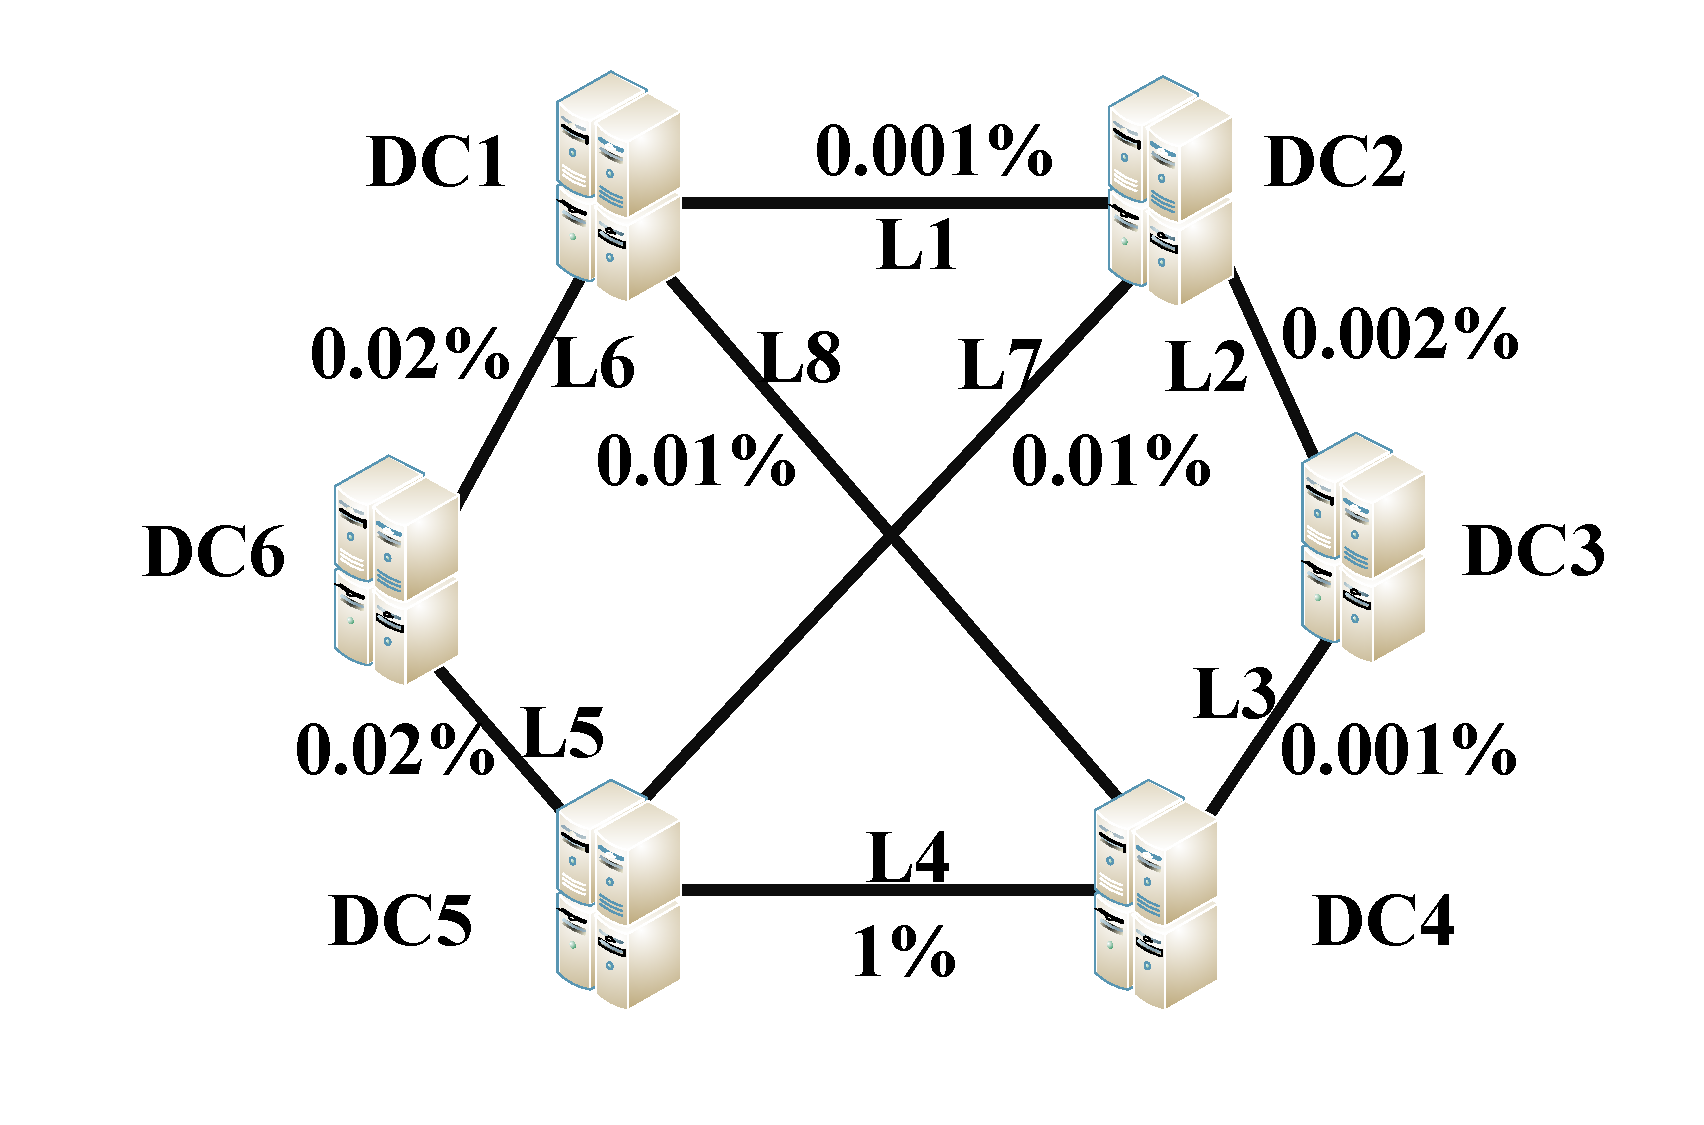
\includegraphics [width=0.8\columnwidth] {fig/testbed.pdf}
%\caption{Testbed topology. }
%\label{testbed}
%\end{center}
%\end{figure}


%In the following part, we also study the impact of probability distribution on performance.



% \begin{figure}
%\begin{center}
%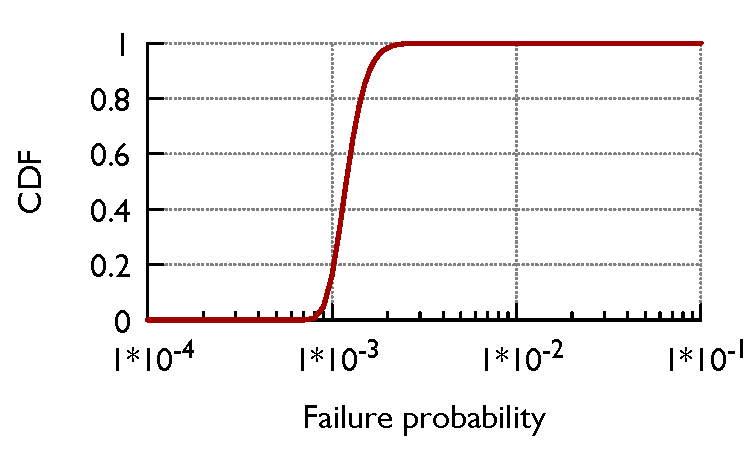
\includegraphics [width=0.8\columnwidth] {fig/weibull.pdf}
%\caption{Weibull distribution  used in our evaluation, where shape and scale parameters are 0.8 and 0.0001, respectively. }
%\label{weibull}
%\end{center}
%\end{figure}








\begin{figure*}[t]
\centering
\subfigure[Bandwidth-based availability]{
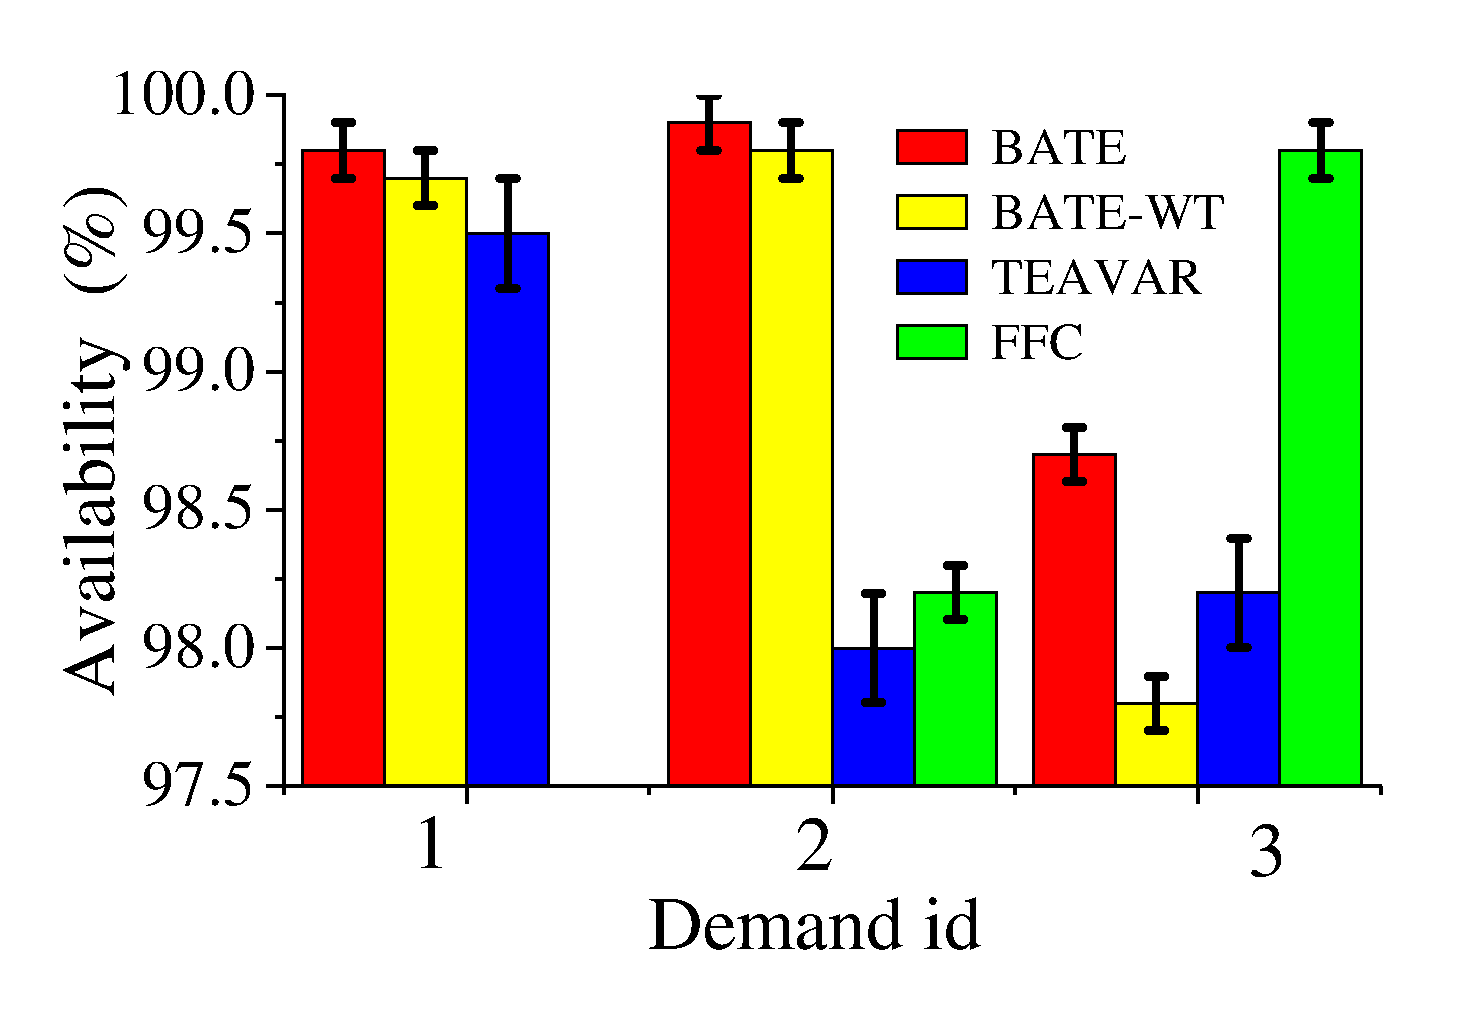
\includegraphics[width=0.24\textwidth]{fig/evaluation/test.pdf}}
\subfigure[Link failures]{
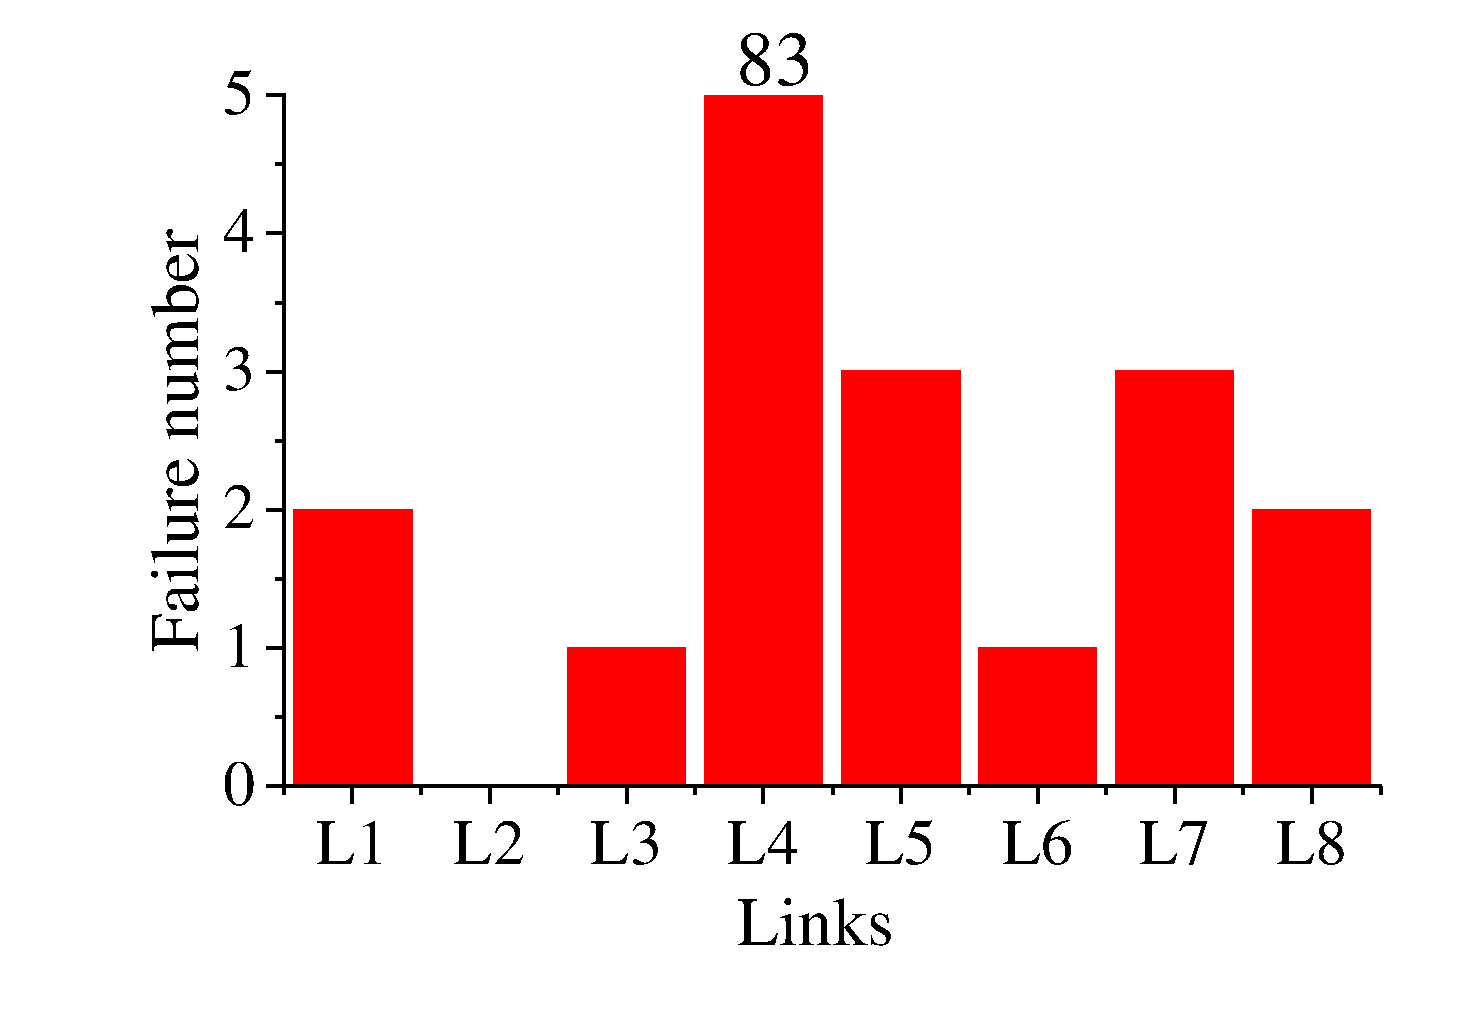
\includegraphics[width=0.24\textwidth]{fig/evaluation/link-failures.pdf}}
%\subfigure[Scheduled results (SWAN)]{
%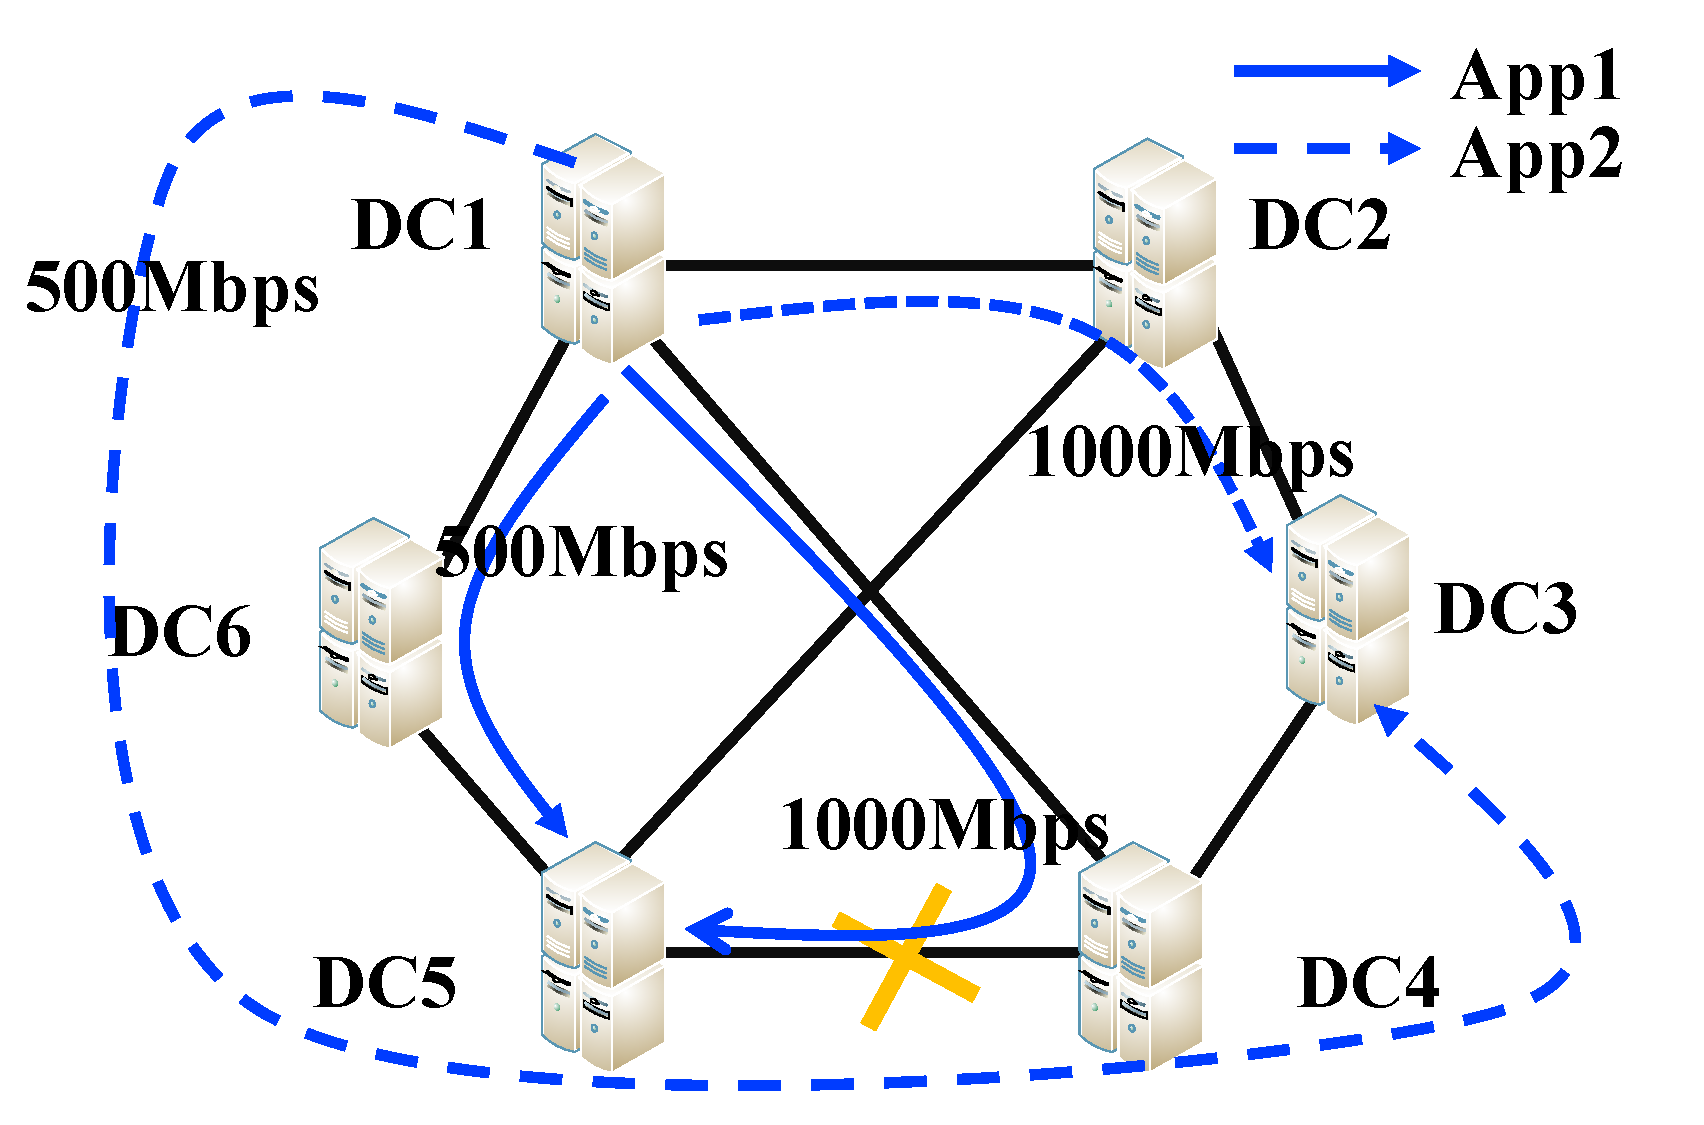
\includegraphics[width=0.19\textwidth]{fig/testbed6.pdf}}
%\subfigure[Measured bandwidth (DC1 to DC3)]{
%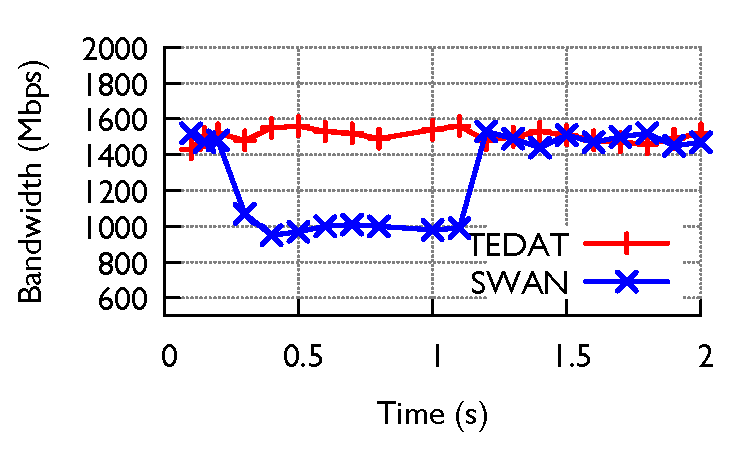
\includegraphics[width=0.19\textwidth]{fig/evaluation/fake/throughput.pdf}}
%\subfigure[Measured bandwidth (DC1 to DC3)]{
%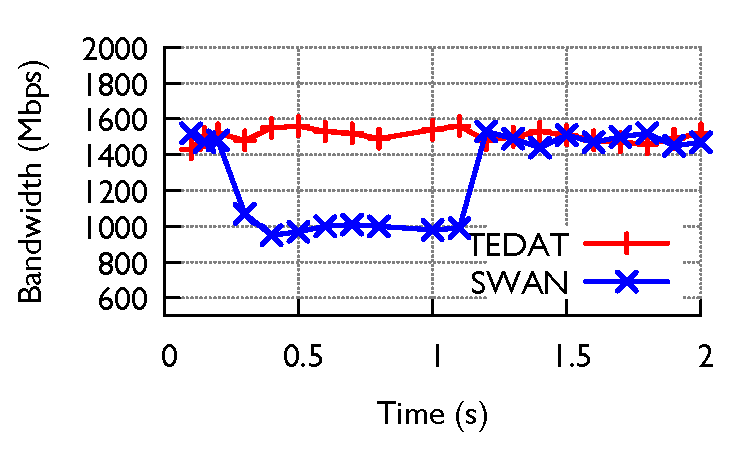
\includegraphics[width=0.19\textwidth]{fig/evaluation/fake/throughput.pdf}}
\subfigure[Data loss ratio]{
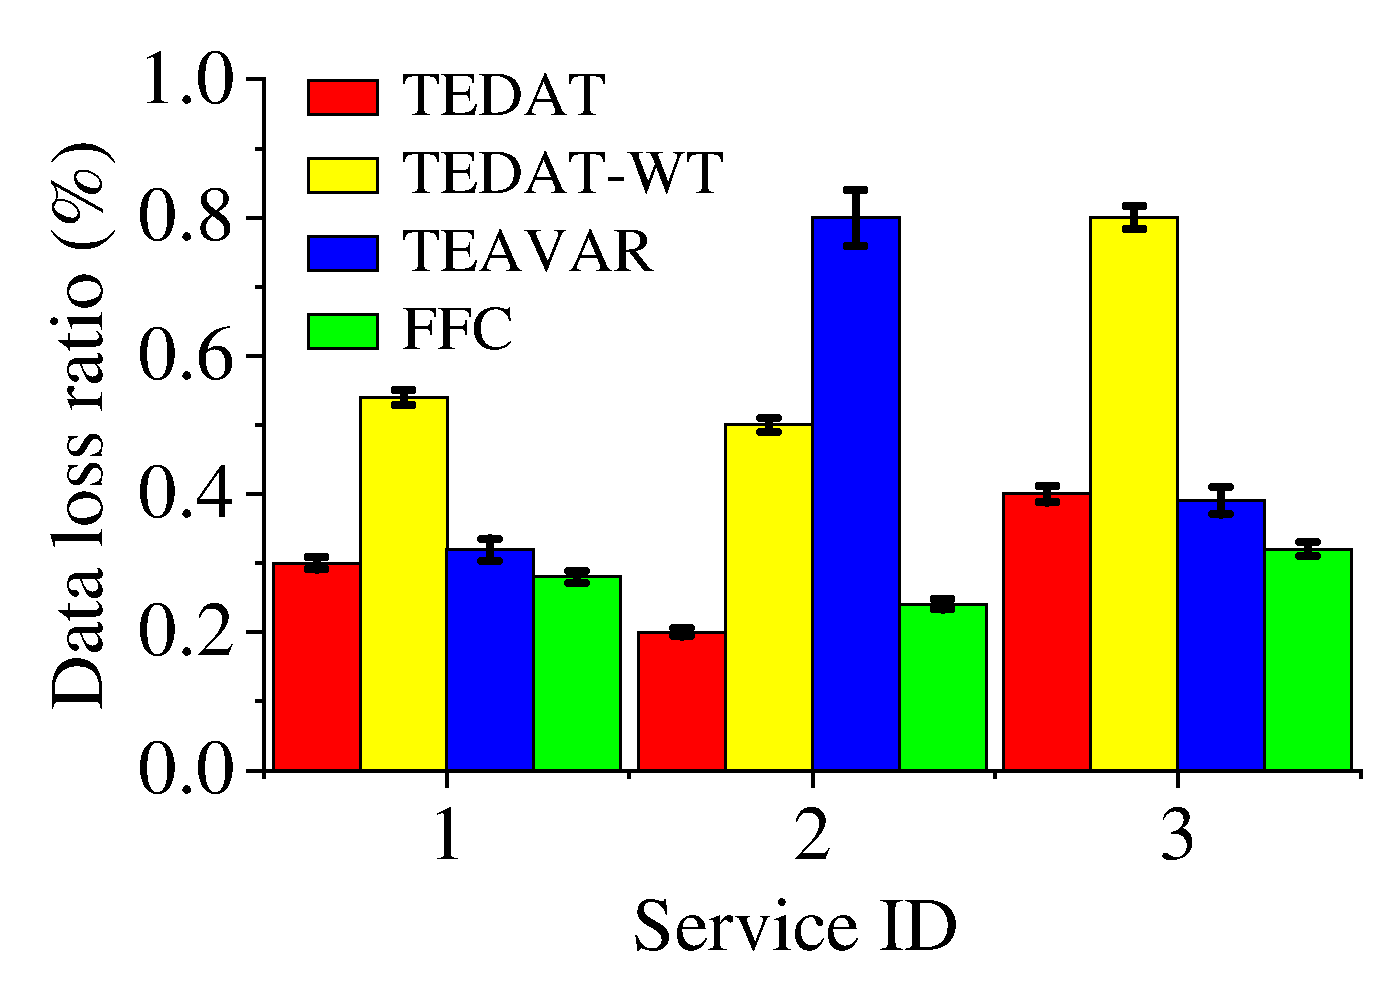
\includegraphics[width=0.24\textwidth]{fig/evaluation/data-loss.pdf}}
%\subfigure[After L4 failure ($\mathsf{BATE}$-1)]{
%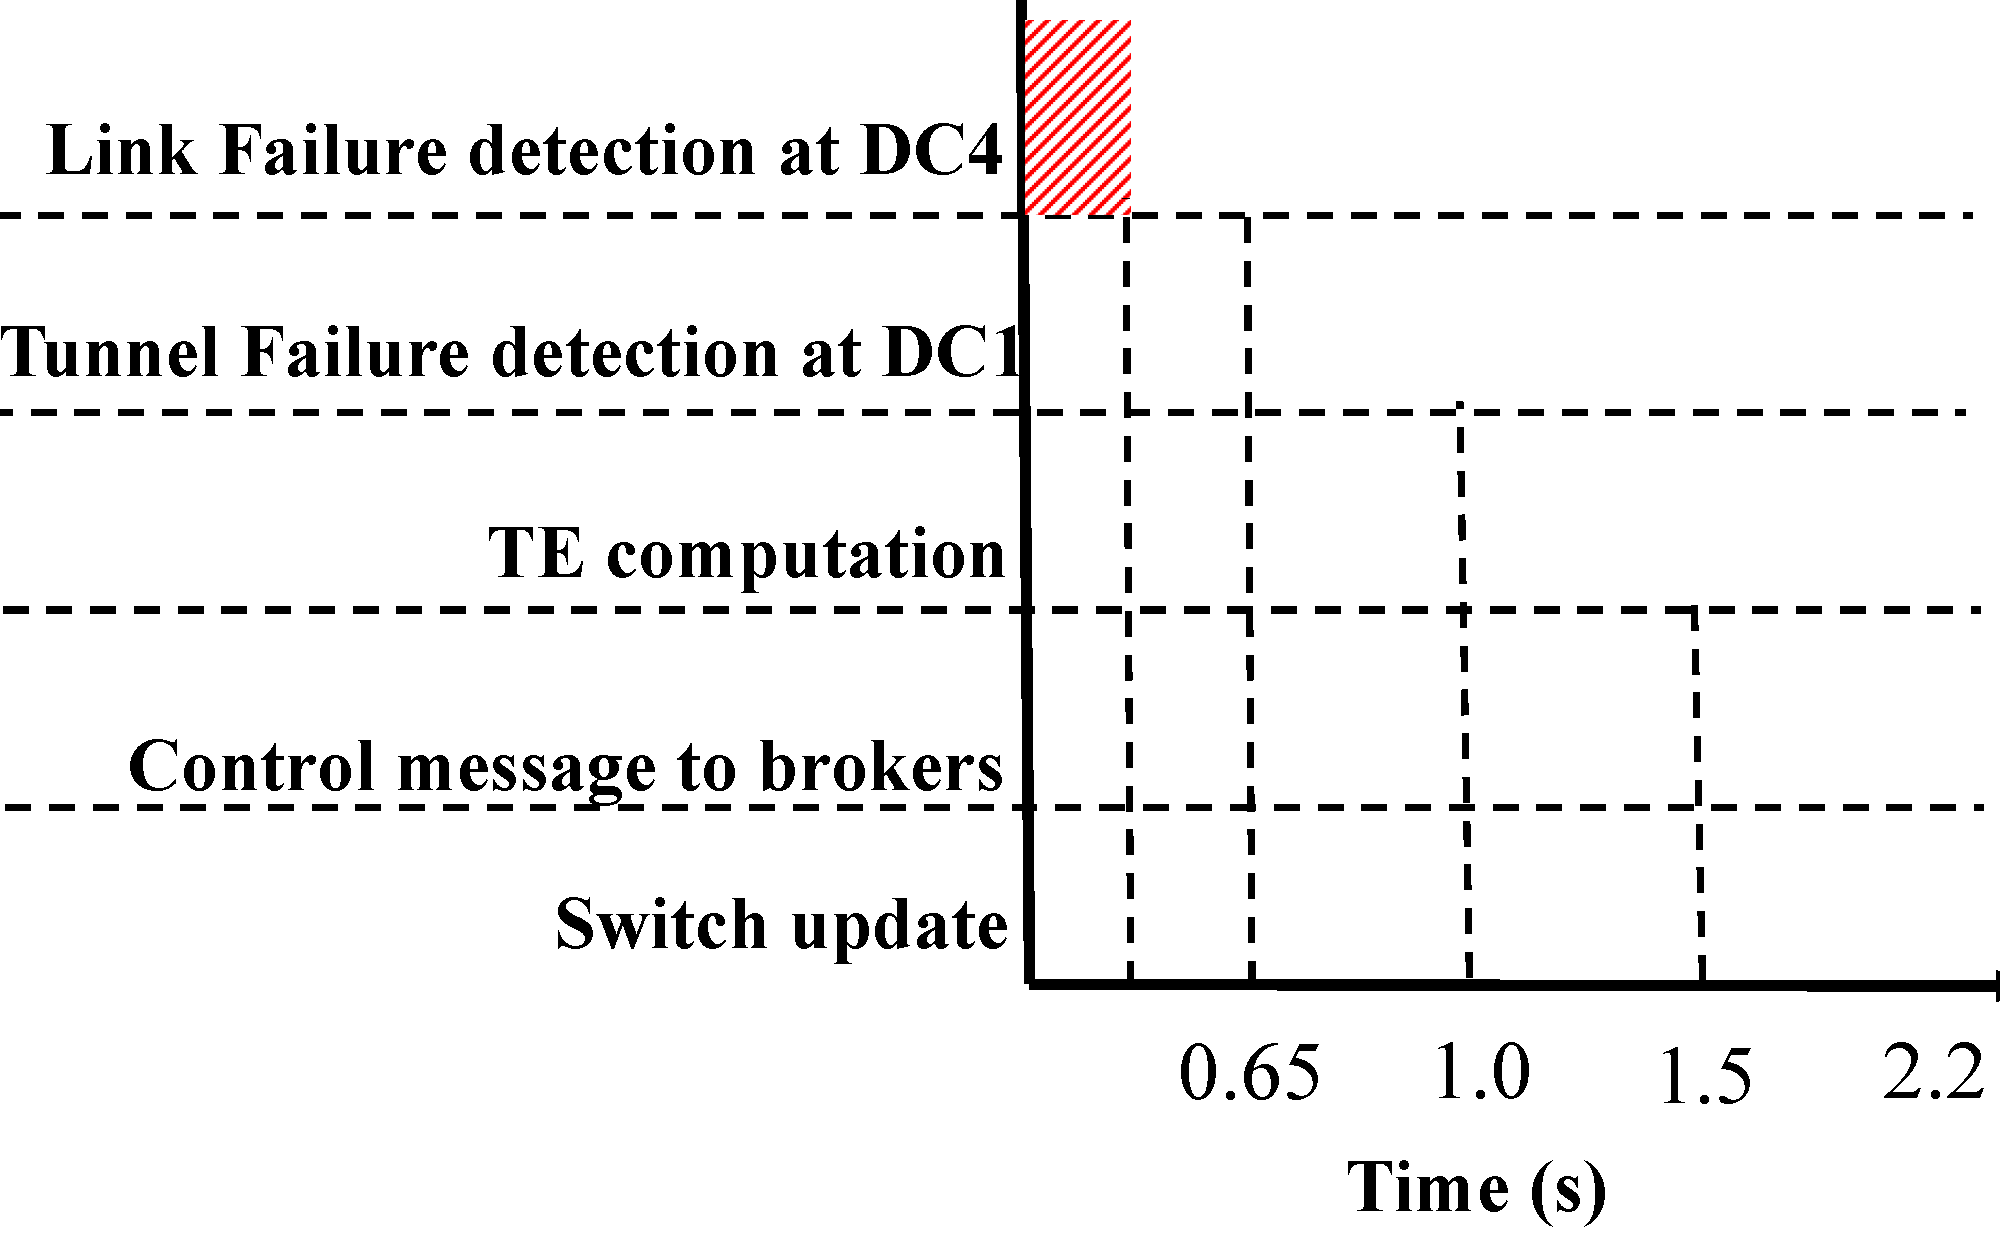
\includegraphics[width=0.24\textwidth]{fig/evaluation/time2.pdf}}
\subfigure[Events after L3 failure]{
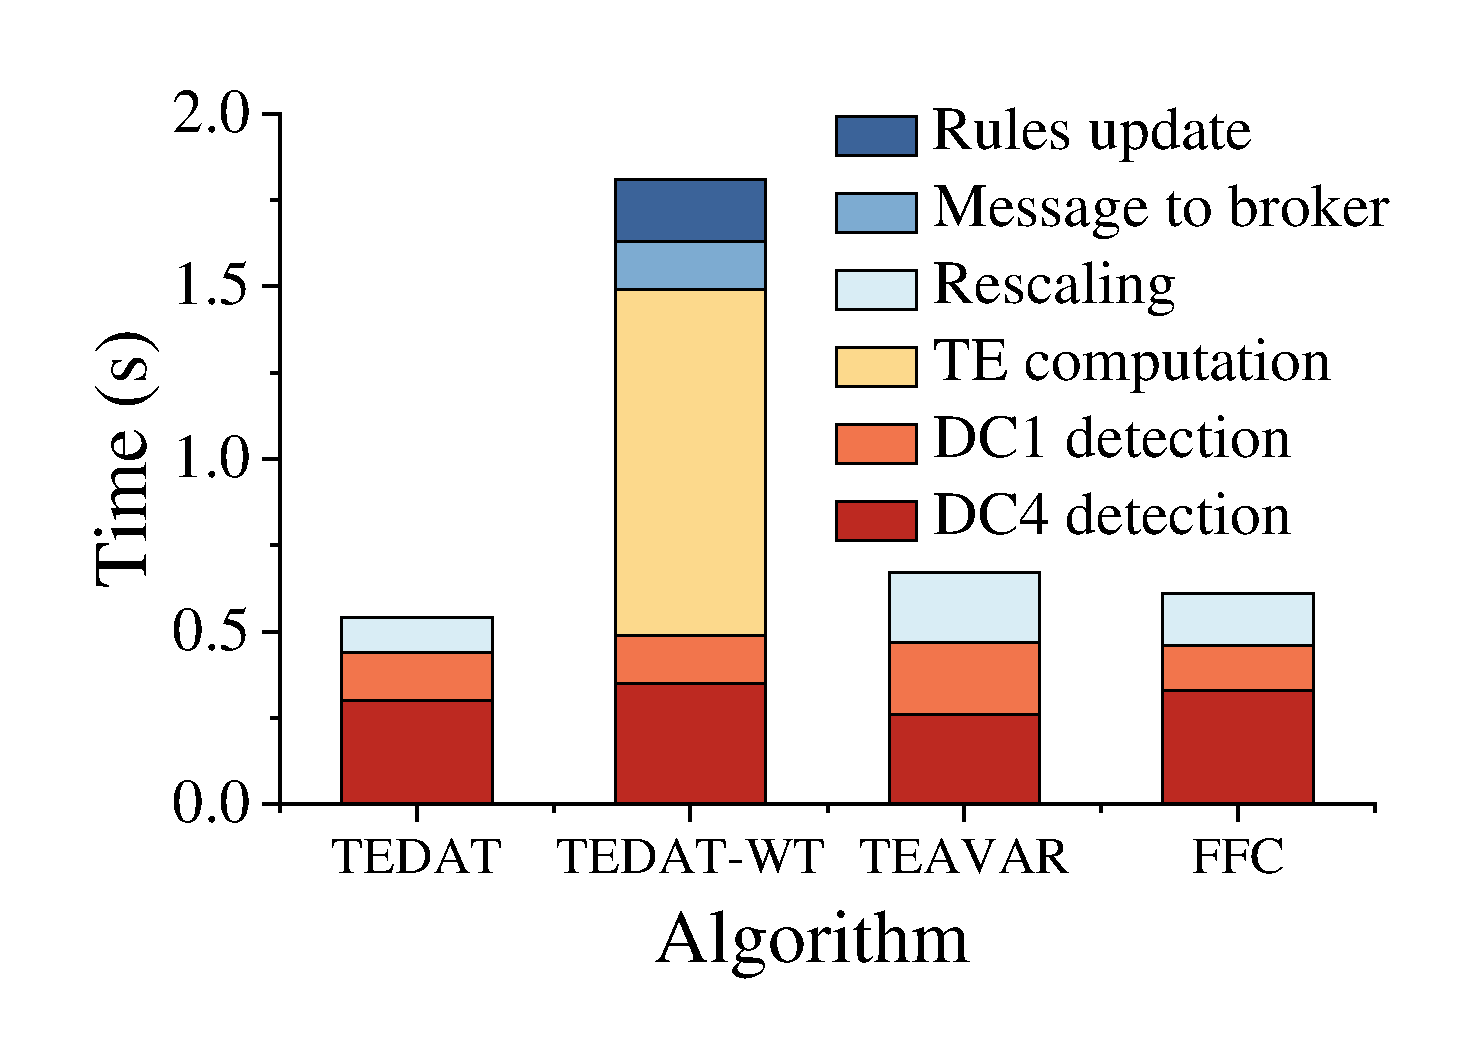
\includegraphics[width=0.24\textwidth]{fig/evaluation/fake-failure.pdf}}

\caption{A private cloud example: we deploy three services whose details are shown in Table \ref{testbed-1}.}
\label{e1}
\end{figure*}






\subsubsection{A public cloud example}
We firstly evaluate a public cloud case.
Assume tenants arrive at the public cloud under poisson process with mean arrival rate 2 every minute and the duration of each bandwidth demand is under exponential distribution with a mean of 5 minutes.
Bandwidth demands between each node pair are under uniform distribution between 10Mbps and 50Mbps.
Every 1Mbps is sold 1$\$$.
%The profit of each tenant (i.e., $w_i$) is proportional to his/her total bandwidth demand.
Availability targets and refunding ratio are randomly chosen from Azure SLAs \cite{azure}.
Each experiment lasts 100 minutes and is repeated 20 times, where the error bars paints the maximal, minimal and mean value.

Figure \ref{e2}(a) demonstrates $\mathsf{BATE}$ only performs slightly worse than the optimal solution (about 4\%) and is at least 2 $\times$ better than the \textit{Fixed} admission control.
This is because $\mathsf{BATE}$ fully considers the availability diversity of tenants.
In contrast, \textit{Fixed} admission control can't change tenants' routing during runtime and such inflexibility leads to higher rejection rate. 
Figure \ref{e2}(b) shows once a tenant's demand is admitted, $\mathsf{BATE}$ can guarantee bandwidth.
FFC and TEAVAR with \textit{Fixed} admission control perform slightly better than when they are without admission control since many tenants' demands are rejected, but they also perform worse than $\mathsf{BATE}$, because FFC is too conservative and and TEAVAR ignores the diverse demands.
Figure \ref{e2}(c) shows $\mathsf{BATE}$ can retain about 15\% more money ratio than FFC and TEAVAR when network fails.
This is because $\mathsf{BATE}$ pre-computes backup allocation with maximal profit and they can be put into practice as far as failures are detected.
We measure total bytes loss according to \textit{iperf} server side reports and packet counters in the switches, then finally derive the data loss ratio.
Figure \ref{e2}(d) demonstrates data loss ratio after network fails, where $\mathsf{BATE}$ performs about 8\% worse than FFC.
FFC performs best since it keeps network utilization low and almost no congestion occurs when network fails, 
while $\mathsf{BATE}$ focuses on Monetary gain rather than data loss.
%, where  FFC-1 and FFC-2 
%denote FFC with and without Fixed admission control,  respectively.
%where TEAVAR-1 and TEAVAR-2 are 
%denote TEAVAR with and without Fixed admission control, 
%We can see that 
%Specially, more than 85\% services achieve  95\% availability under $\mathsf{BATE}$, while only about 73\% and 60\%  services achieve this target under TEAVAR and FFC.
%Figure \ref{e2}(c) illustrates three schemes have similar performance for services with small availability target (i.e., $<95\%$).
%However, for services with large availability targets (i.e., $>=99\%)$,  $\mathsf{BATE}$ performs up to  20\% and 30\% better than TEAVAR and FFC.
%The reason for this is that $\mathsf{BATE}$ considers the diverse availability demands, so services with large targets can plunder
%bandwidth from others.
%Compared with TEAVAR, 20\% more applications satisfy their bandwidth demand with $\mathsf{BATE}$.
%Figure  \ref{e2}(c) shows the scheduled results with the same parameters.
%We can see the results approximate to that shown in Figure \ref{e2}(b).
%The gap is narrow, about 5\% on average.
%In the following evaluation, we develop a simulator to perform trace-driven simulations.
%Figure \ref{e2}(d) demonstrates the availability deviation between the testbed and simulation under the same parameters.
%We can see that the error is narrow, i.e., more than 90\% time the difference is less than 5\%.




%
%\begin{equation}
%\forall  j \in J : g_j=
%\begin{cases}
%\alpha &\text{$S_j \ge \beta_j$}\\
%\mu(R_j)  &\text{$S_j < \beta_j$}
%\end{cases}
%\label{availability2}
%\end{equation}




%\textbf{Metrics.}
%We examine the performance of different TE schemes with respect to throughput, availability satisfaction ratio and achieved availability.

%\textbf{Optimization.}
%Our traffic engineering optimization framework uses Gurobi LP solver\cite{gurobi} to solve the optimization problems.


\subsubsection{A private cloud example}\label{testbedresults}

%In this part we will perform experiments on our testbed to evaluate the performance of  $\mathsf{BATE}$.
 \begin{table}
\scriptsize
\centering
\caption{Scheduled results of different schemes.}\label{testbed-1}
\renewcommand{\arraystretch}{1.0}
\begin{tabular}{|c|l|l|l|l|ll} \hline
\setlength{\tabcolsep}{10pt}
{Service}&\multicolumn{1}{|c|}{paths}&\multicolumn{1}{|c|}{$\mathsf{BATE}$}&\multicolumn{1}{|c|}{TEAVAR}&\multicolumn{1}{|c|}{FFC}\\
\hline
&{DC1$\to$DC2$\to$DC3}&0&500&0\\
{Service-1}&{DC1$\to$DC4$\to$DC3}&1000&500&250\\
(99.5\%)&{DC1$\to$DC2$\to$DC5$\to$DC4$\to$DC3}&0&0&0\\
&{DC1$\to$DC4$\to$DC5$\to$DC2$\to$DC3}&0&0&0\\
\hline
&{DC1$\to$DC4}&0&250&0\\
{Service-2}&{DC1$\to$DC2$\to$DC5$\to$DC4}&0&0&0\\
(99.9\%)&{DC1$\to$DC2$\to$DC3$\to$DC4}&500&0&250\\
&{DC1$\to$DC6$\to$DC5$\to$DC4}&0&250&250\\
\hline
&{DC1$\to$DC2$\to$DC5}&500&500&750\\
{Service-3}&{DC1$\to$DC4$\to$DC5}&0&250&0\\
(95\%)&{DC1$\to$DC6$\to$DC5}&1000&750&750\\
&{DC1$\to$DC2$\to$DC3$\to$DC4$\to$DC5}&0&0&0\\
%&&&{DC1$\to$DC4$\to$DC5$\to$DC2$\to$DC3}&{750}\\
%&&&{DC1$\to$DC2$\to$DC3}&{0}\\
%&&&{DC1$\to$DC4$\to$DC3}&{0}\\
%{service-1}&&\multirow{2}{*}{{TEAVAR}}&{DC1$\to$DC2$\to$DC3}&{750}\\
%(95\%)&&&{DC1$\to$DC4$\to$DC3}&{750}\\
%&&\multirow{2}{*}{{SWAN}}&{DC1$\to$DC2$\to$DC3}&{1000}\\
%&&&{DC1$\to$DC4$\to$DC3}&{500}\\
%\hline
%&\multirow{6}{*}{500}&\multirow{2}{*}{{$\mathsf{BATE}$}}&{DC1$\to$DC4}&{250}\\
%&&&{DC1$\to$DC2$\to$DC3$\to$DC4}&{250}\\
%{service-2}&&\multirow{2}{*}{{TEAVAR}}&{DC1$\to$DC4}&{250}\\
%(99.99\%)&&&{DC1$\to$DC6$\to$DC5$\to$DC4}&{250}\\
%&&{{SWAN}}&{DC1$\to$DC4}&{500}\\
%\hline
%&\multirow{4}{*}{500}&{{$\mathsf{BATE}$}}&{DC1$\to$DC6$\to$DC5}&{500}\\
%{service-3}&&\multirow{2}{*}{{TEAVAR}}&{DC1$\to$DC6$\to$DC5}&{250}\\
%(90\%)&&&{DC1$\to$DC2$\to$DC5}&{250}\\
%&&{{SWAN}}&{DC1$\to$DC6$\to$DC5}&{500}\\
\hline
\end{tabular}
\end{table}
We now test the performance under a simple private cloud example, where three services are deployed and all admitted.
Service-1 is from DC1 to DC3, Service-2 is from DC1 to DC4 and Service-3 is from DC1 to DC5.
Their bandwidth demands are 1000Mbps, 500Mbps and 1500Mbps, respectively.
Assume the availability targets of Service-1 , Service-2 and Service-3 are  99.5\%, 99.9\% and 95\%, respectively.
All services last 100s and each experiment repeats 100 times,  where the error bars paints the maximal, minimal and mean value.
$\mathsf{BATE}$-WT refers $\mathsf{BATE}$ without failure recovery.

Figure \ref{e1}(a) shows the bandwidth-based availability which is measured as the time qualification ratio. A second is regarded as qualified if the gap between total measured bandwidth and bandwidth demand is less than 1\%.
We can see that all services can reach their availability targets under $\mathsf{BATE}$, while Service-1 fails under FFC and Service-2 fails under both TEAVAR and FFC.
To explore the reason, we show the scheduled results of the three schemes in TABLE \ref{testbed-1}:  
(1) FFC reserves too much bandwidth to protect routing and service1 is unable to gain enough bandwidth;
(2) $\mathsf{BATE}$ abandons link L4 for Service-2, while TEAVAR adopts it.
According to the link failure times shown in Figure \ref{e1}(b), we can see that most failures are from link L4 in our experiment.
Although TEAVAR considers link failure probability, it ignores the availability targets of different services.
Therefore, Service-3 gains redundant bandwidth and affects Service-2 finally.
%During L4 failure, service2 is unable to gain enough bandwidth. 
%and it will take much time for the controller to retrieve from congestion.
%All links are up under normal circumstances and the probability of this scenario is 98.9\%.
%We now consider a scenario in which DC4-DC5 link fails and other links are up.
%The probability of this failure scenario is about 1\%, which is about 10 $\times$ larger than the probability sum of other failure scenarios.
%We disable the link between DC4 and DC5 at $t=0.2s$ to produce this scenario.
%Figure \ref{e1}(c) shows aggregate bandwidth from DC1 to DC3.
%We can see SWAN drops about 33\% bandwidth between 0.2s and 1.1s.
%The result of service1 is similar.
Data loss mainly comes from congestion and blackhole, where congestion losses are always link oversubscribed and blackhole losses occur during the time between a link fails and ingress switch rescale.
Figure \ref{e1}(c) demonstrates $\mathsf{BATE}$ and FFC performs better than   $\mathsf{BATE}$-WT  and TEAVAR for data losses ratio.
Data losses of Service-2 under TEAVAR is high due to Link L4 failings.
$\mathsf{BATE}$-WT performs worse than the other three schemes, because it takes much time to derive new resource allocation when network fails and the events time of  $\mathsf{BATE}$-WT shown in Figure \ref{e1}(d) just prove this.
%We can see that $\mathsf{BATE}$-1 and FFC performs better than   $\mathsf{BATE}$-2  and TEAVAR.
%The losses of TEAVAR mainly comes from link $L4$ failure which is adopt by Service-2.
%When L3 fails, DC1 and DC4 take about 0.4s to detect the failure.
%$\mathsf{BATE}$-1 can  rescale traffic with the backup allocation results, therefore, packet losses will stop immediately.
%Control messages distributing and switch updating take about 0.3s, while the most time-consuming operation is TE computation which takes about 1s, 
%therefore, $\mathsf{BATE}$-2 performs relatively worse than other schemes.
%$\mathsf{BATE}$ considers link failure probability as well as the diverse demands of services \textit{proactively}, as a result, the time consuming events shown in Figure  \ref{e1}(c) rarely happens.






%We can see that SWAN has largest average link utilization, but for links with small failure probability, $\mathsf{BATE}$ is higher used.
%This is because some low probability failure links under $\mathsf{BATE}$ are kept high utilized to guarantee bandwidth demands.

%Figure \ref{topologyutilization}(a) shows the average total link utilization for different schemes when traffic scale is 2.
%We can see that average link utilization of $\mathsf{BATE}$ is about 10\% larger than TEAVAR but 10\% lower than Max-Min.
%Figure \ref{topologyutilization}(b)  shows the average link utilization for links with low failure probability.
%We can see that low failure probability links under $\mathsf{BATE}$ are at least 10\% higher utilized than Max-min scheme.
%This demonstrates that $\mathsf{BATE}$ achieves right balance between link utilization and availability. 
%\begin{figure*}[t]
%\centering
%\subfigure[IBM]{
%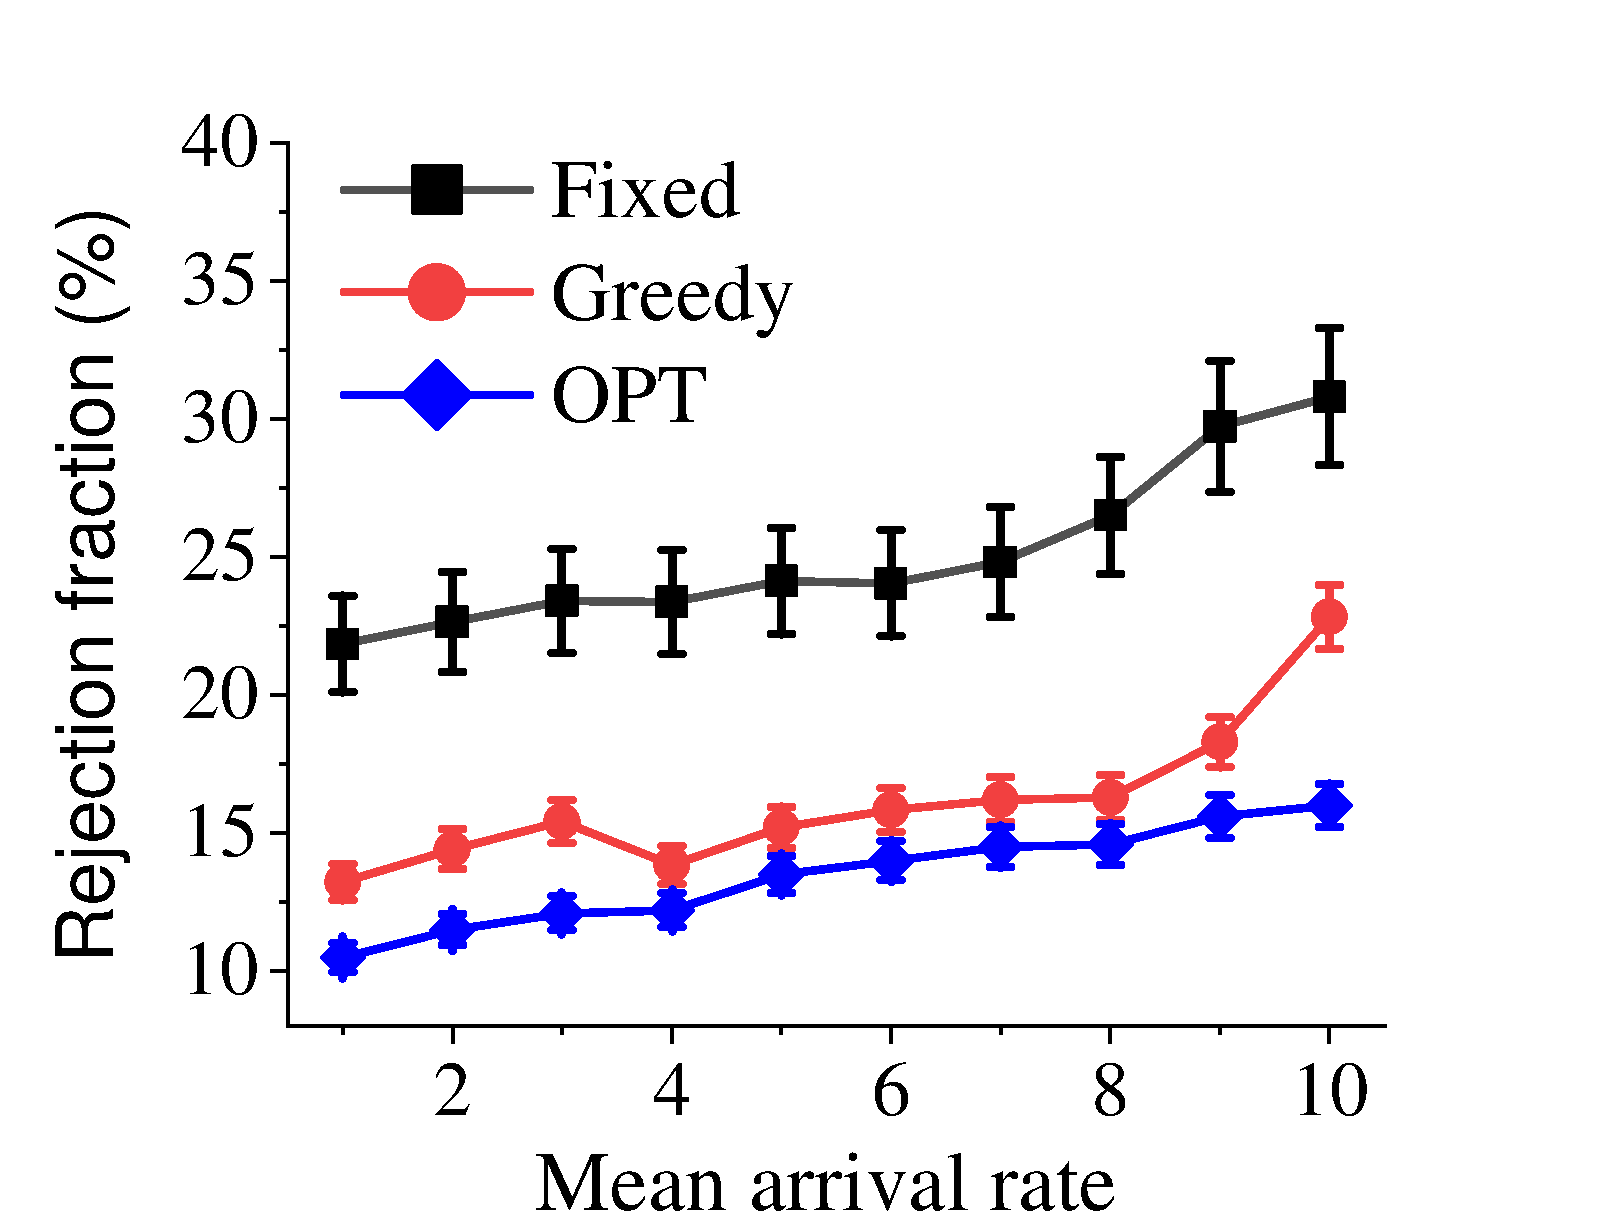
\includegraphics[width=0.24\textwidth]{fig/evaluation/IBM-admit.pdf}}
%\subfigure[B4 ]{
%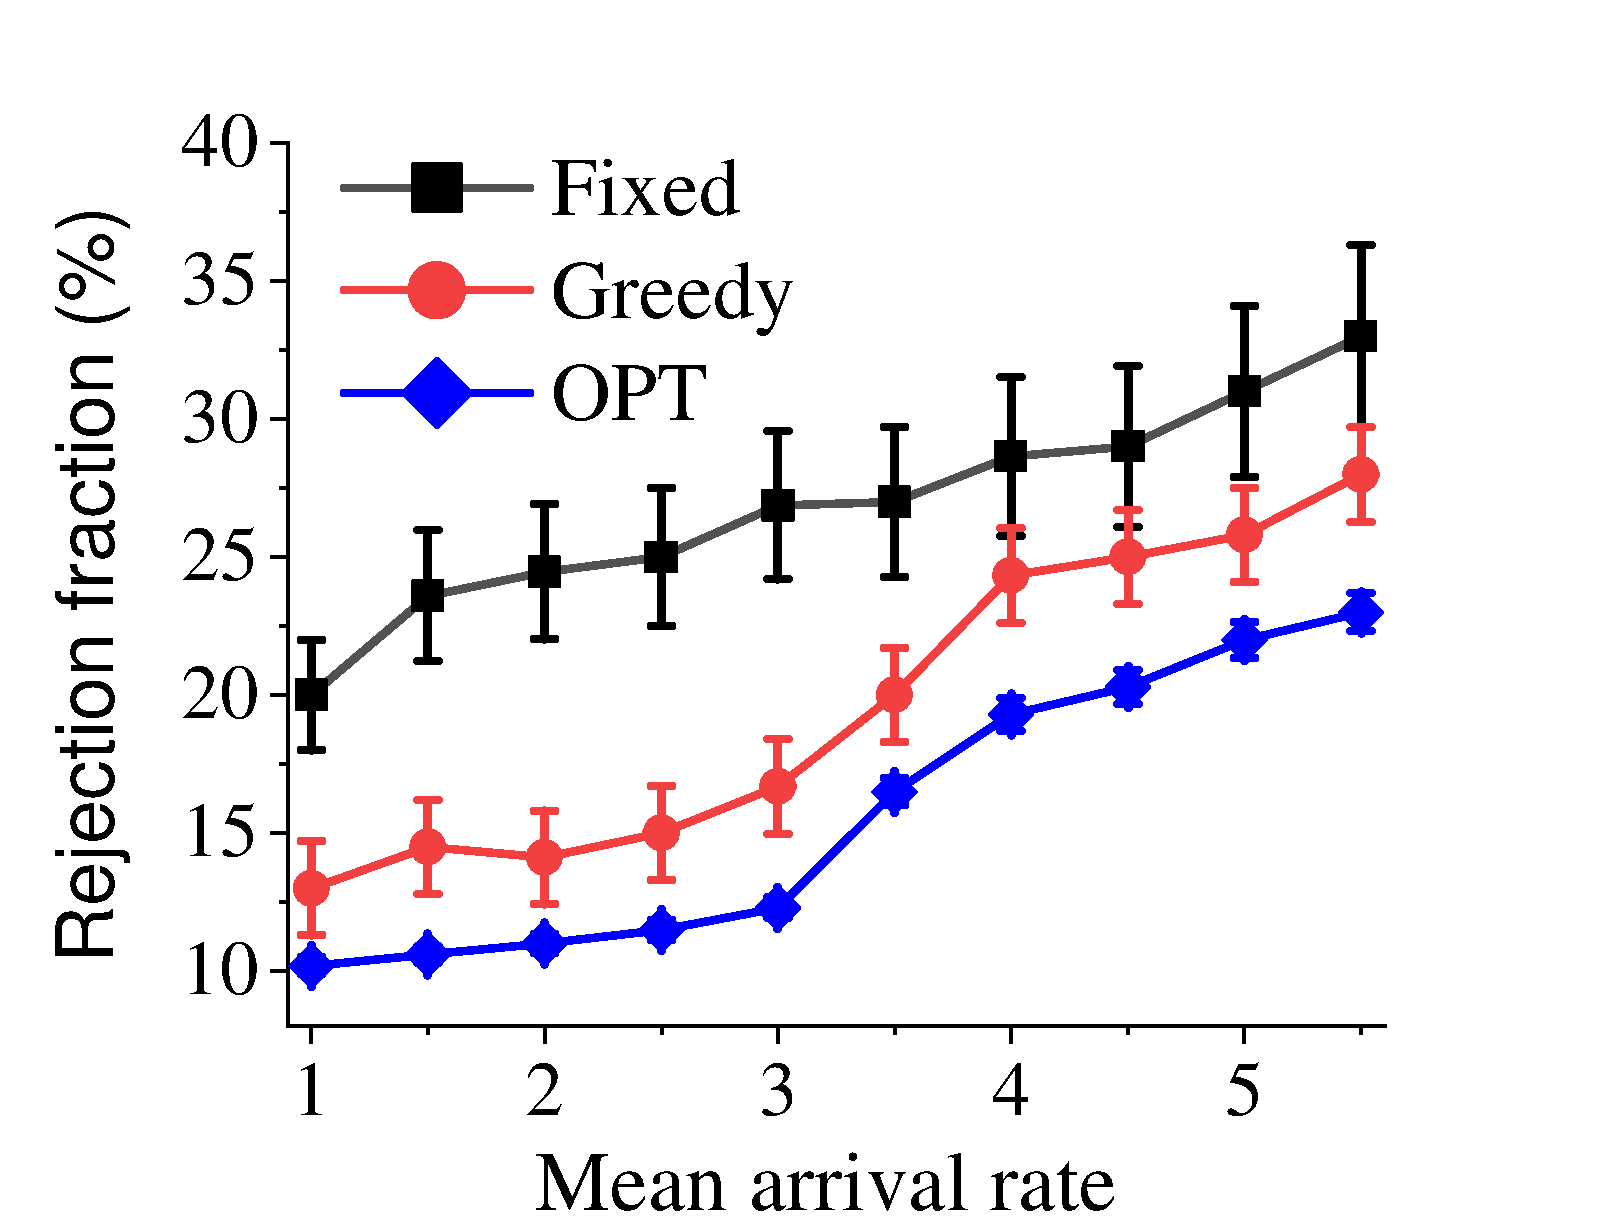
\includegraphics[width=0.24\textwidth]{fig/evaluation/b4-admit.pdf}}
%\subfigure[ATT]{
%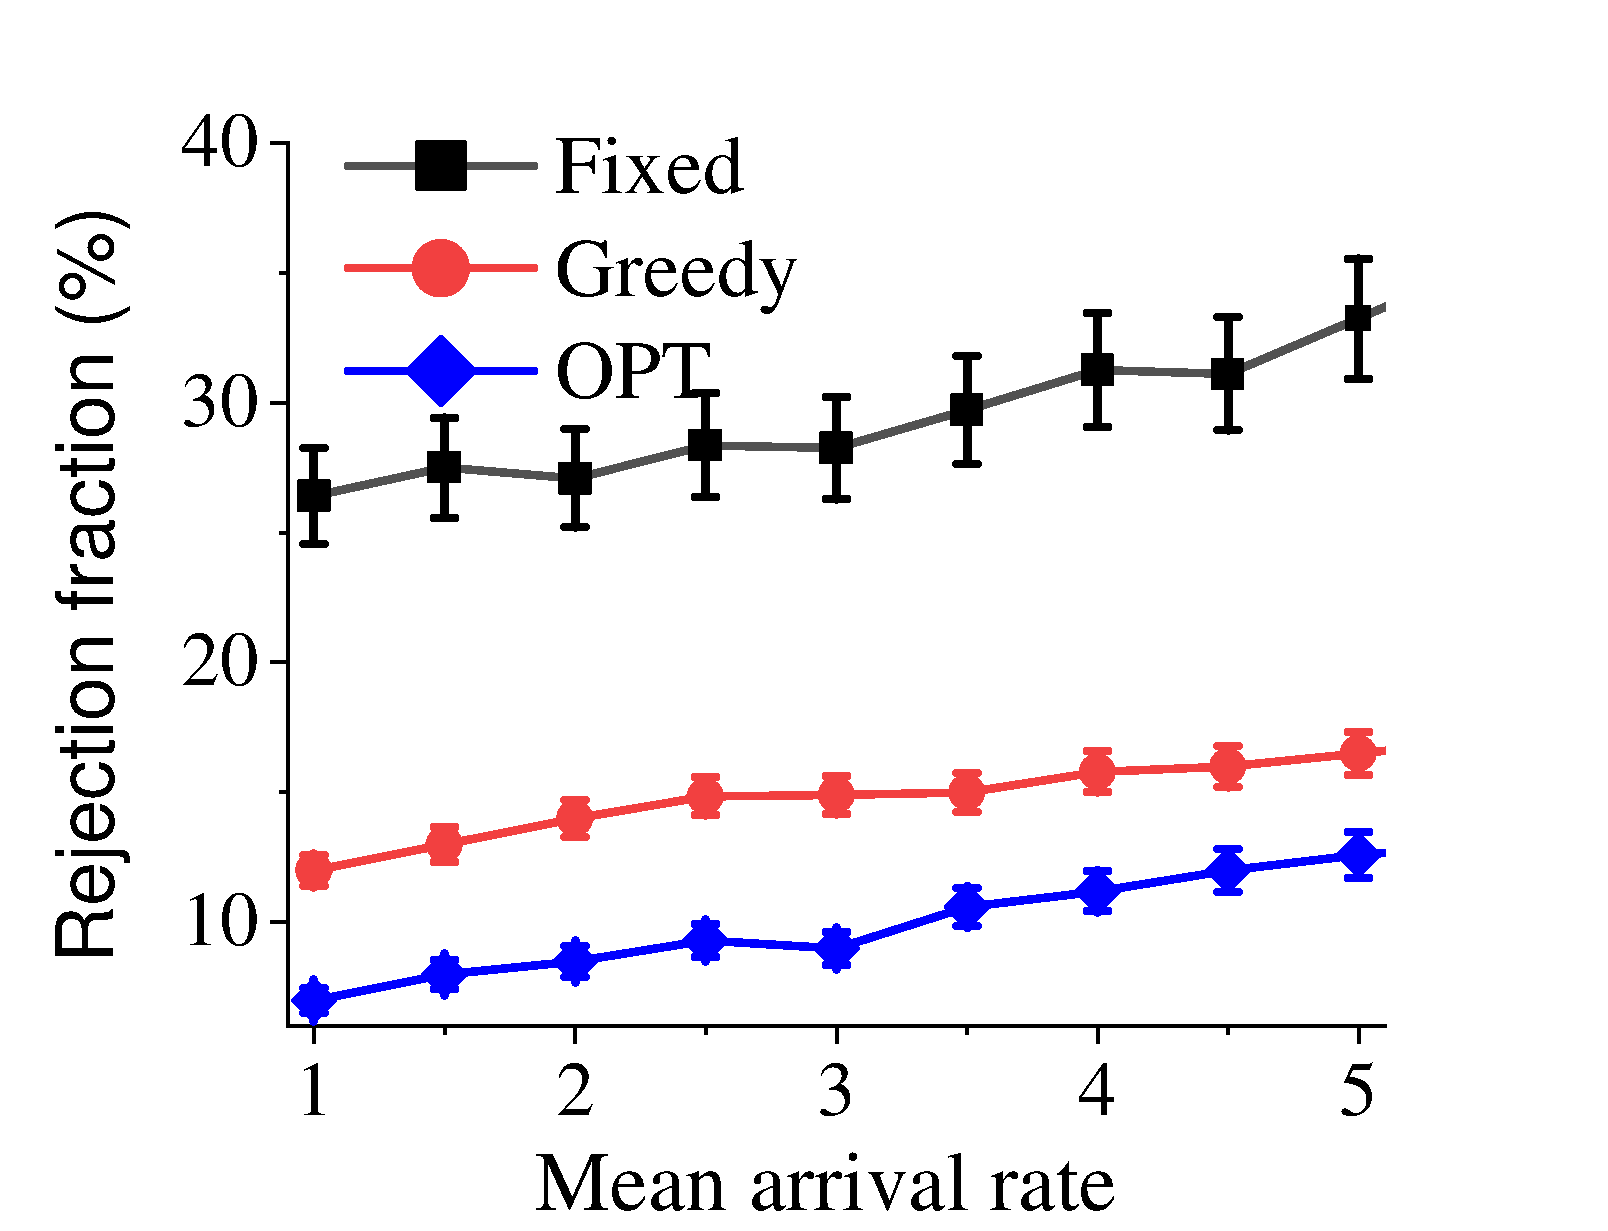
\includegraphics[width=0.24\textwidth]{fig/evaluation/att-admit.pdf}}
%\subfigure[Cernet]{
%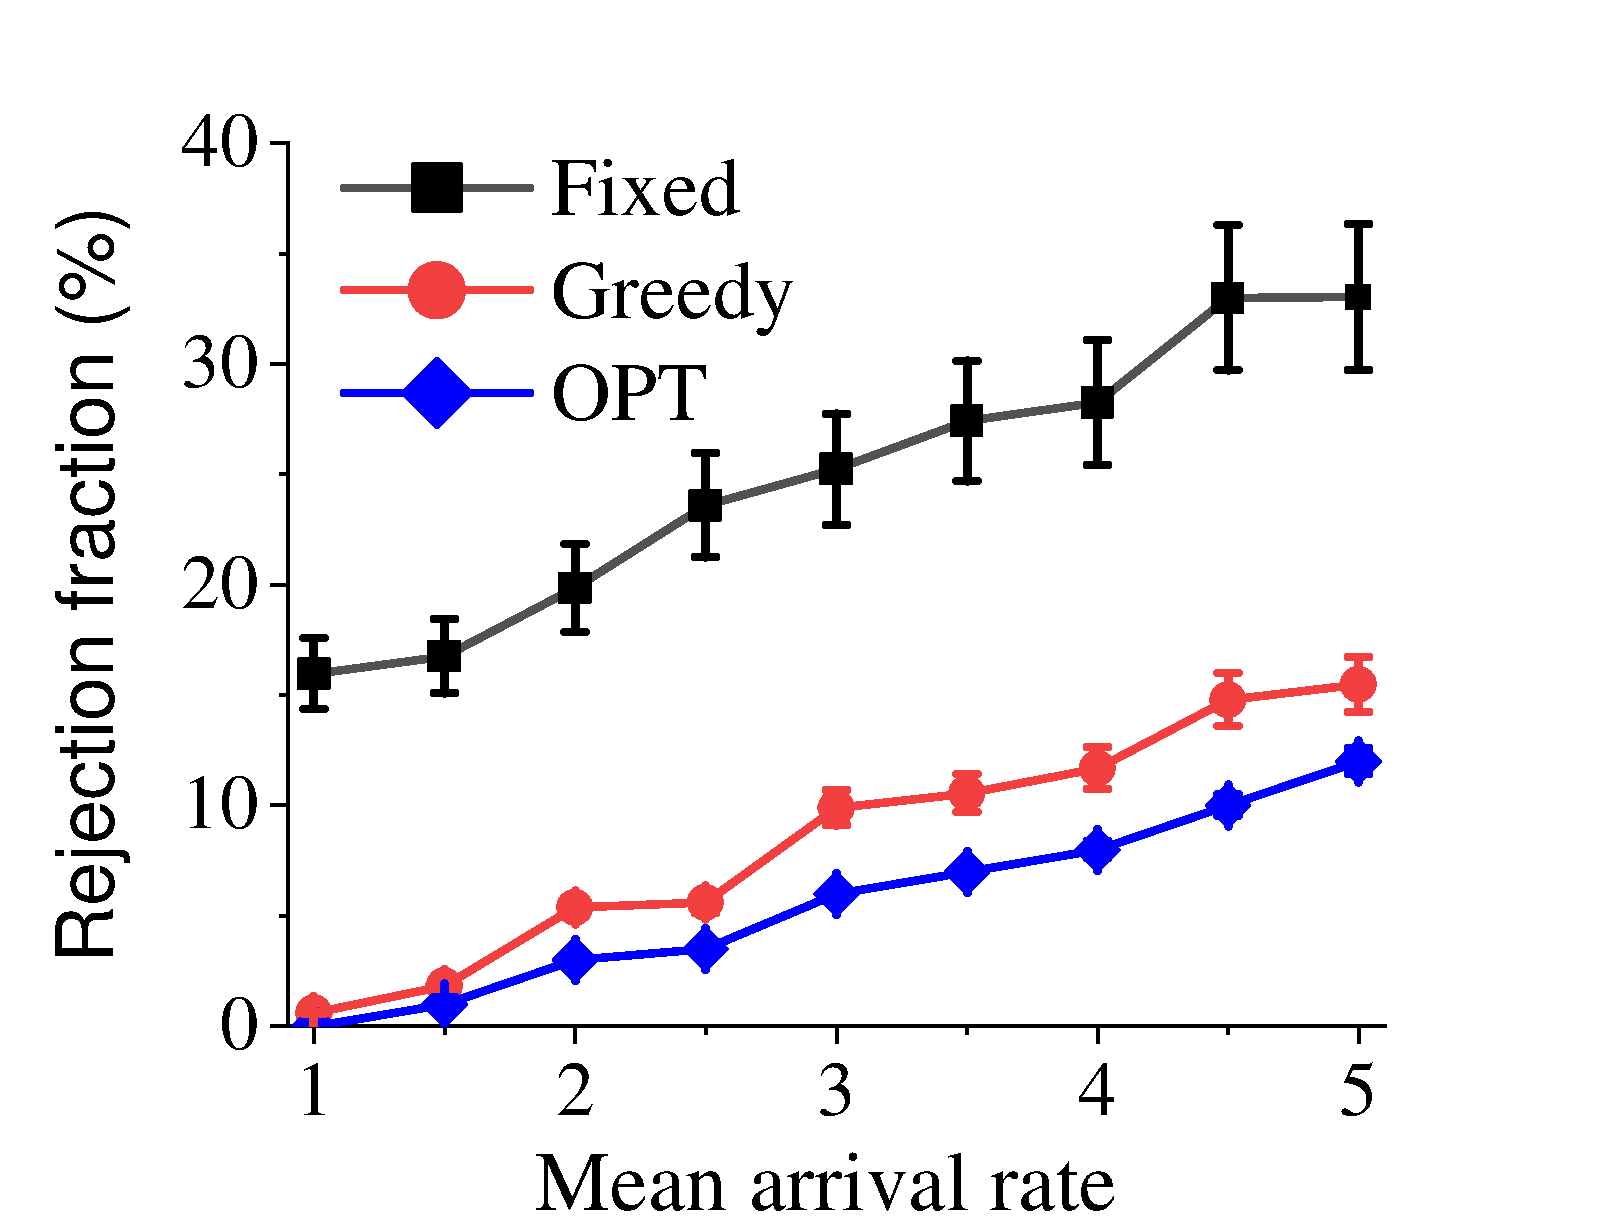
\includegraphics[width=0.24\textwidth]{fig/evaluation/cernet-admit.pdf}}
%\caption{$\mathsf{BATE}$ vs. Fixed admission control scheme under different network topologies.  All requests in (a) and (b) arrive with Poisson Process. Requests in (c) arrive with Gaussian Process. Requests in (d) arrive with Poisson Process whose mean arrival rate is 6.  }
%\label{availability_fig1}
%\end{figure*}

\begin{table}
\centering
\caption{Network topologies used in the simulations}\label{evaluation-topologies}
\renewcommand{\arraystretch}{1.0}
\begin{tabular}{|c|c|c|c|c|c|c|c|c|c|c|} \hline
\setlength{\tabcolsep}{10pt}
\textbf{Topology Name}&\textbf{\#Nodes}&\textbf{\#Links}\\
\hline
IBM&18&48\\
\hline
B4&12&38\\
\hline
ATT&25&112\\
\hline
CERNET2&14&32\\
\hline
\end{tabular}
\end{table}

\begin{figure*}[t]
\centering
%\begin{tabular}{c}
%
\includegraphics[width=0.7\textwidth]{fig/evaluation/legend.pdf}
%\end{tabular}
%\vfill
\subfigure[IBM]{
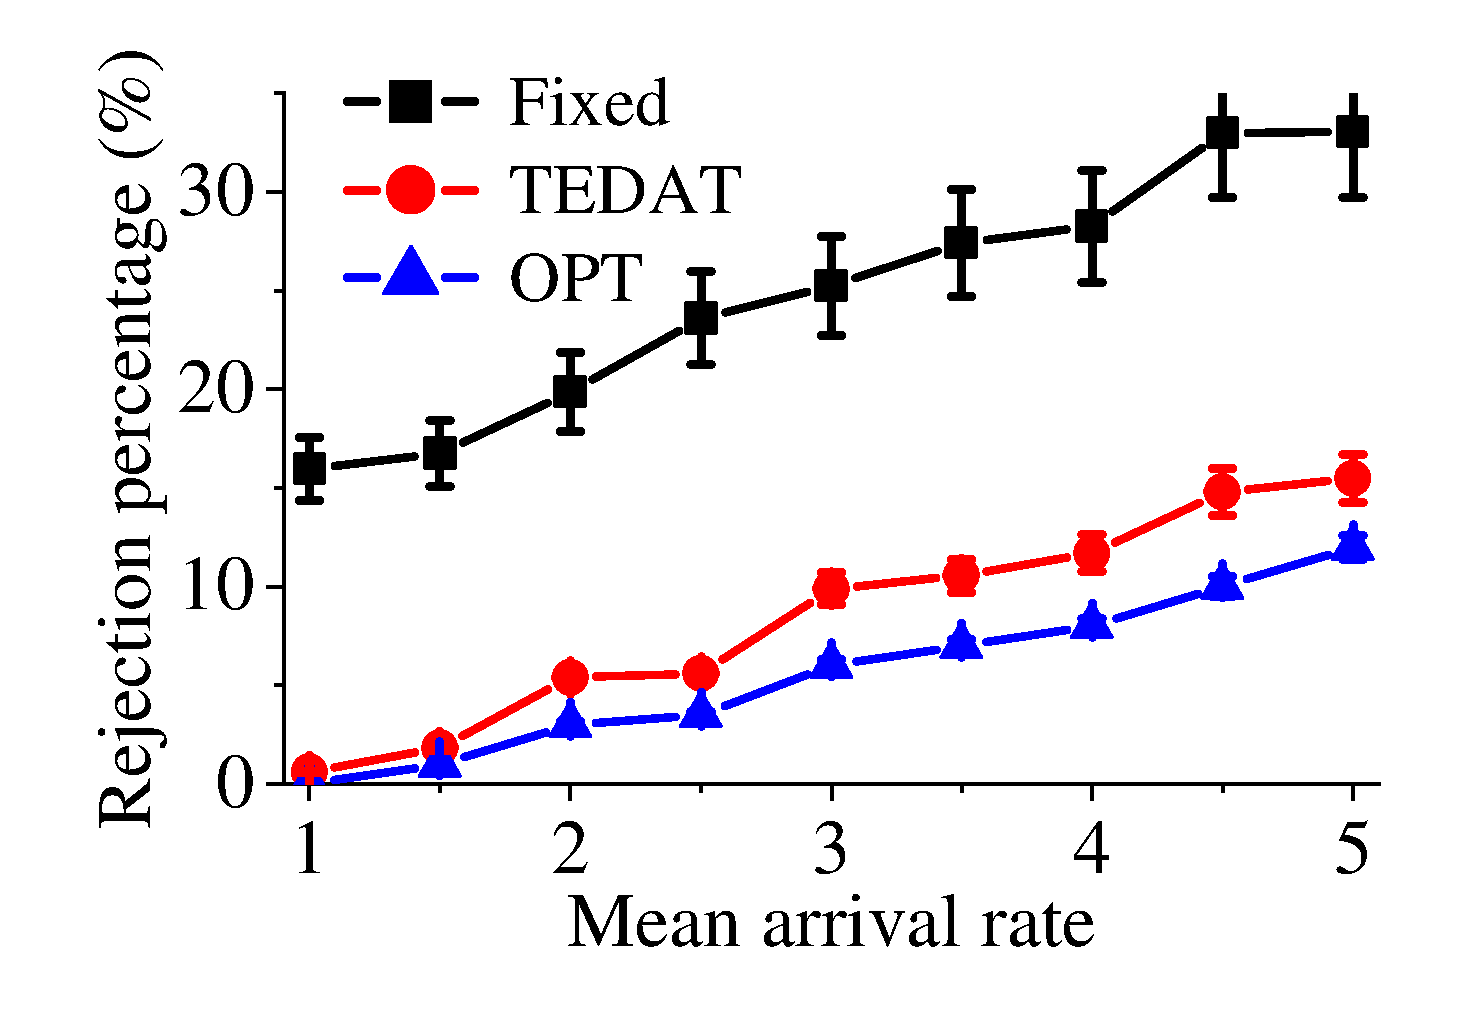
\includegraphics[width=0.24\textwidth]{fig/evaluation/sim-admit.pdf}}
\subfigure[B4 ]{
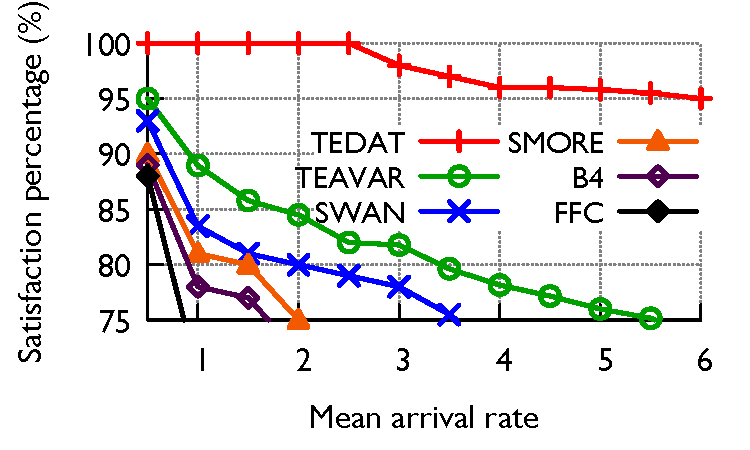
\includegraphics[width=0.24\textwidth]{fig/evaluation/att.pdf}}
\subfigure[ATT]{
\includegraphics[width=0.24\textwidth]{fig/evaluation/cernet3.pdf}}
\subfigure[Cernet]{
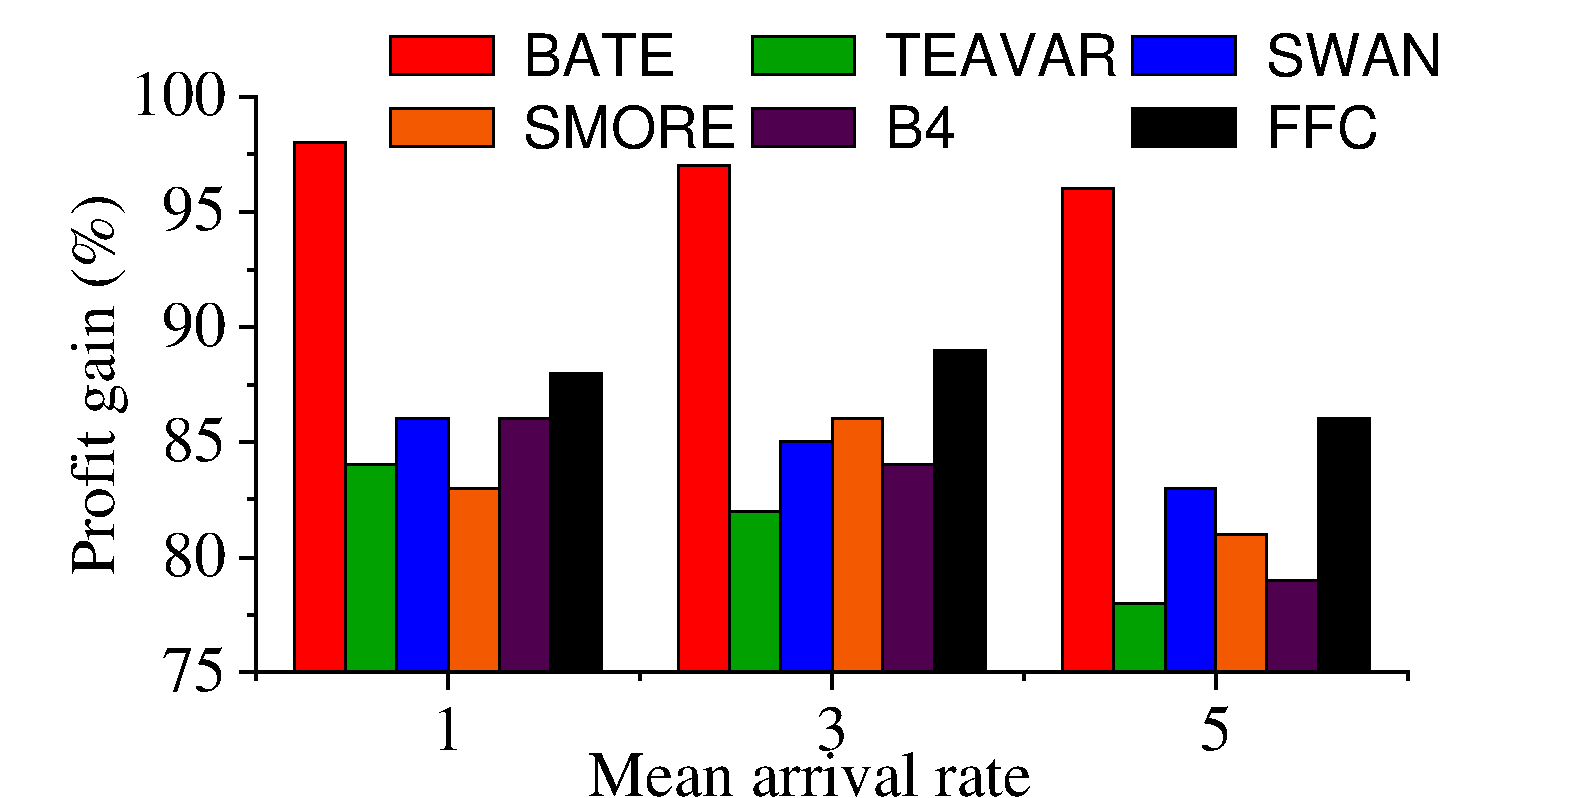
\includegraphics[width=0.24\textwidth]{fig/evaluation/sim-monney.pdf}}
\caption{$\mathsf{BATE}$  vs. various schemes under different network topologies.}
\label{availability_fig1}
\end{figure*}



\begin{figure}
\centering
\subfigure[Link utilization]{
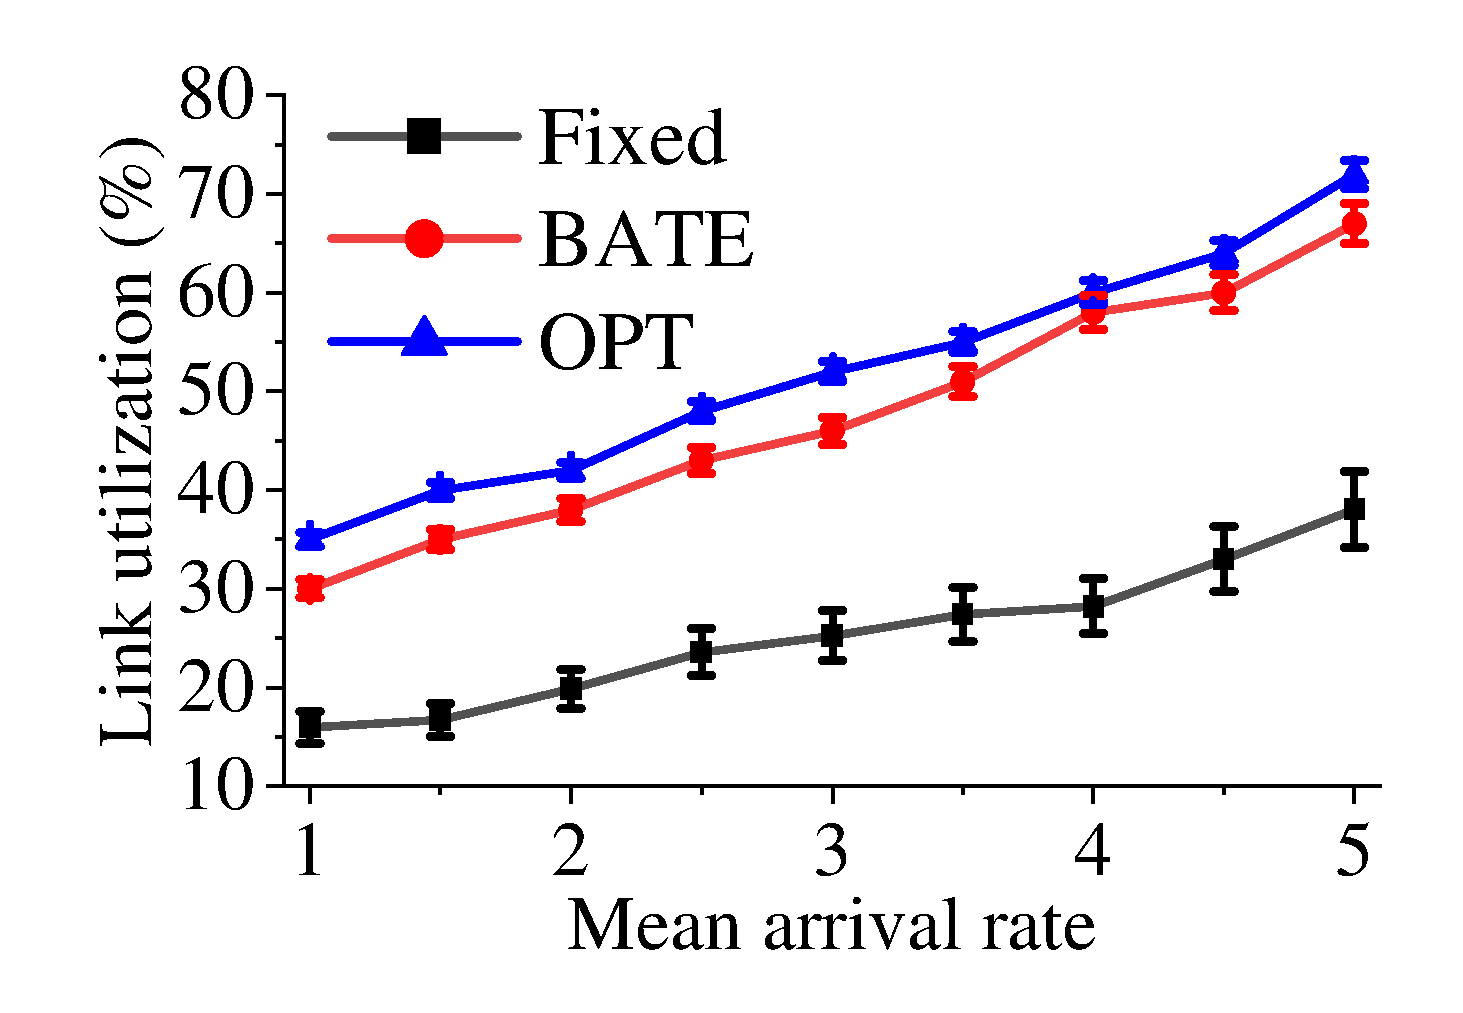
\includegraphics[width=0.23\textwidth]{fig/evaluation/link-utilization.pdf}}
\subfigure[Admission time]{
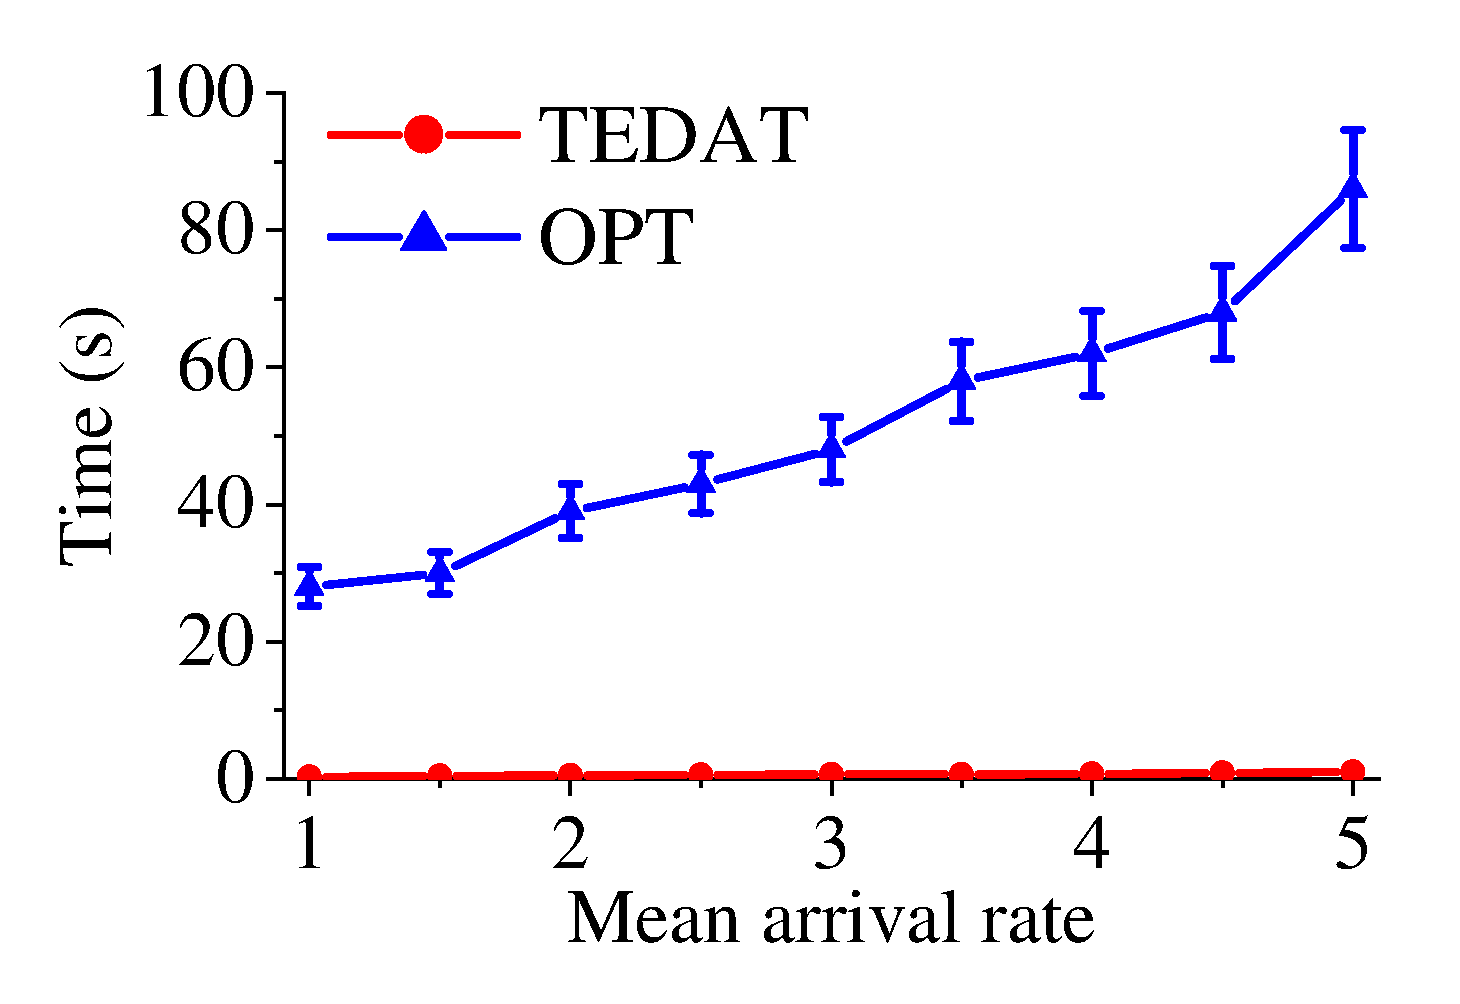
\includegraphics[width=0.23\textwidth]{fig/evaluation/admission-control-time.pdf}}
\caption{Scalability of admission control.}
\label{admission-benefit}
\end{figure}




%\begin{figure*} 
%   \begin{minipage}[t]{0.25\linewidth} 
%    \centering 
%    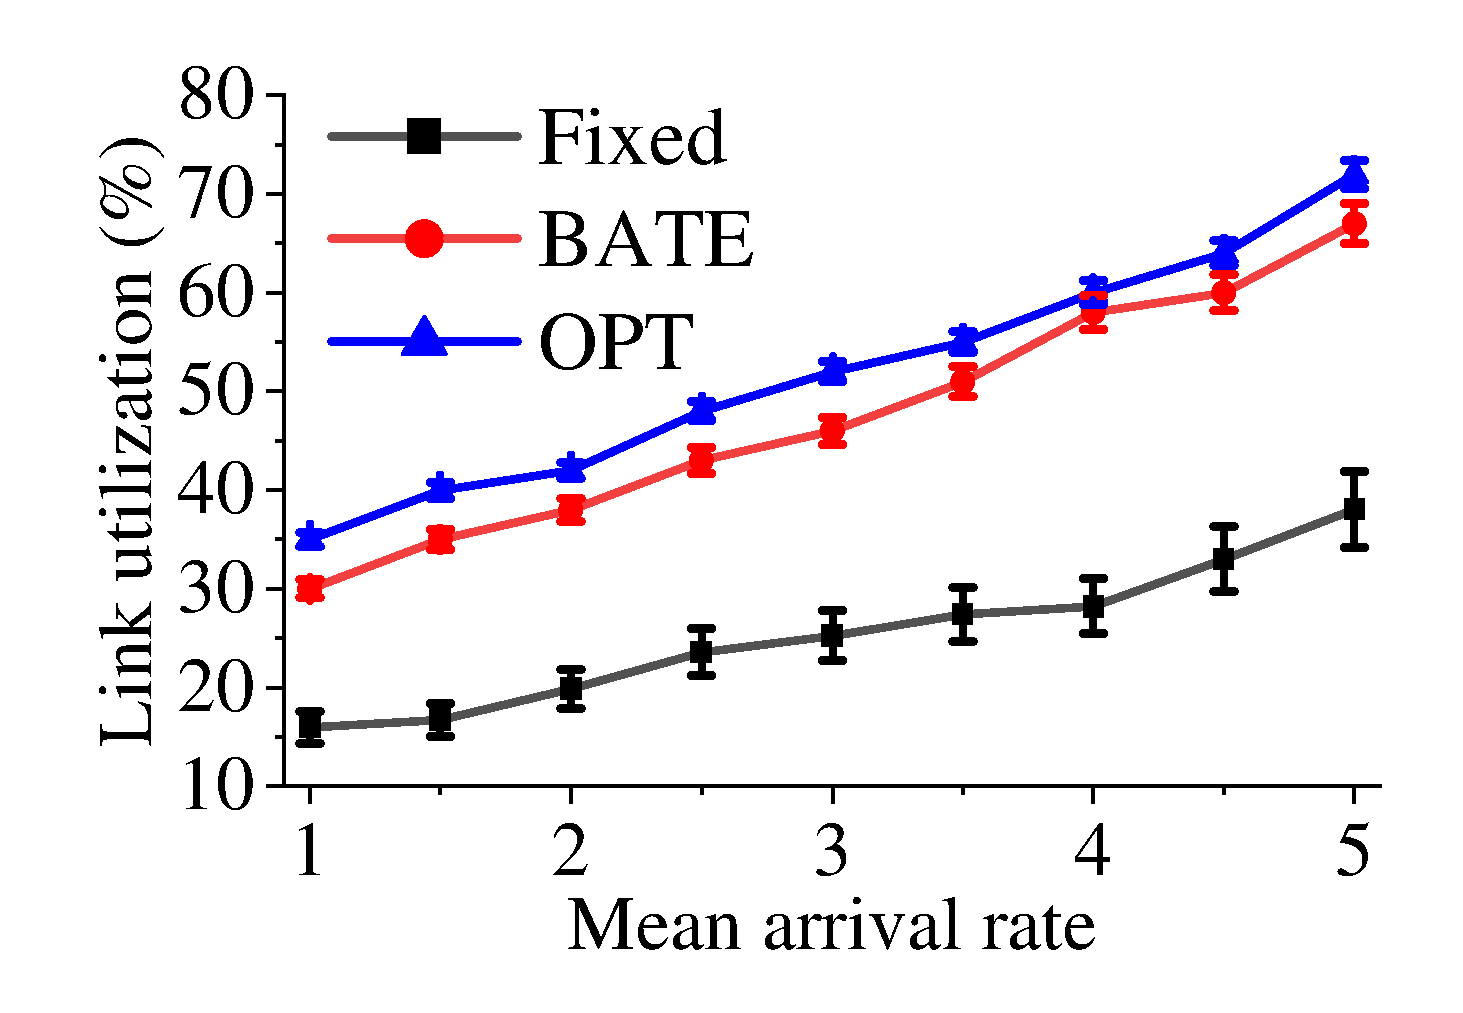
\includegraphics[width=1.8 in]{fig/evaluation/link-utilization.pdf}
%    \caption{Weight difference.} 
%    \label{fig-weight} 
%  \end{minipage}% 
%   \begin{minipage}[t]{0.25\linewidth} 
%    \centering 
%    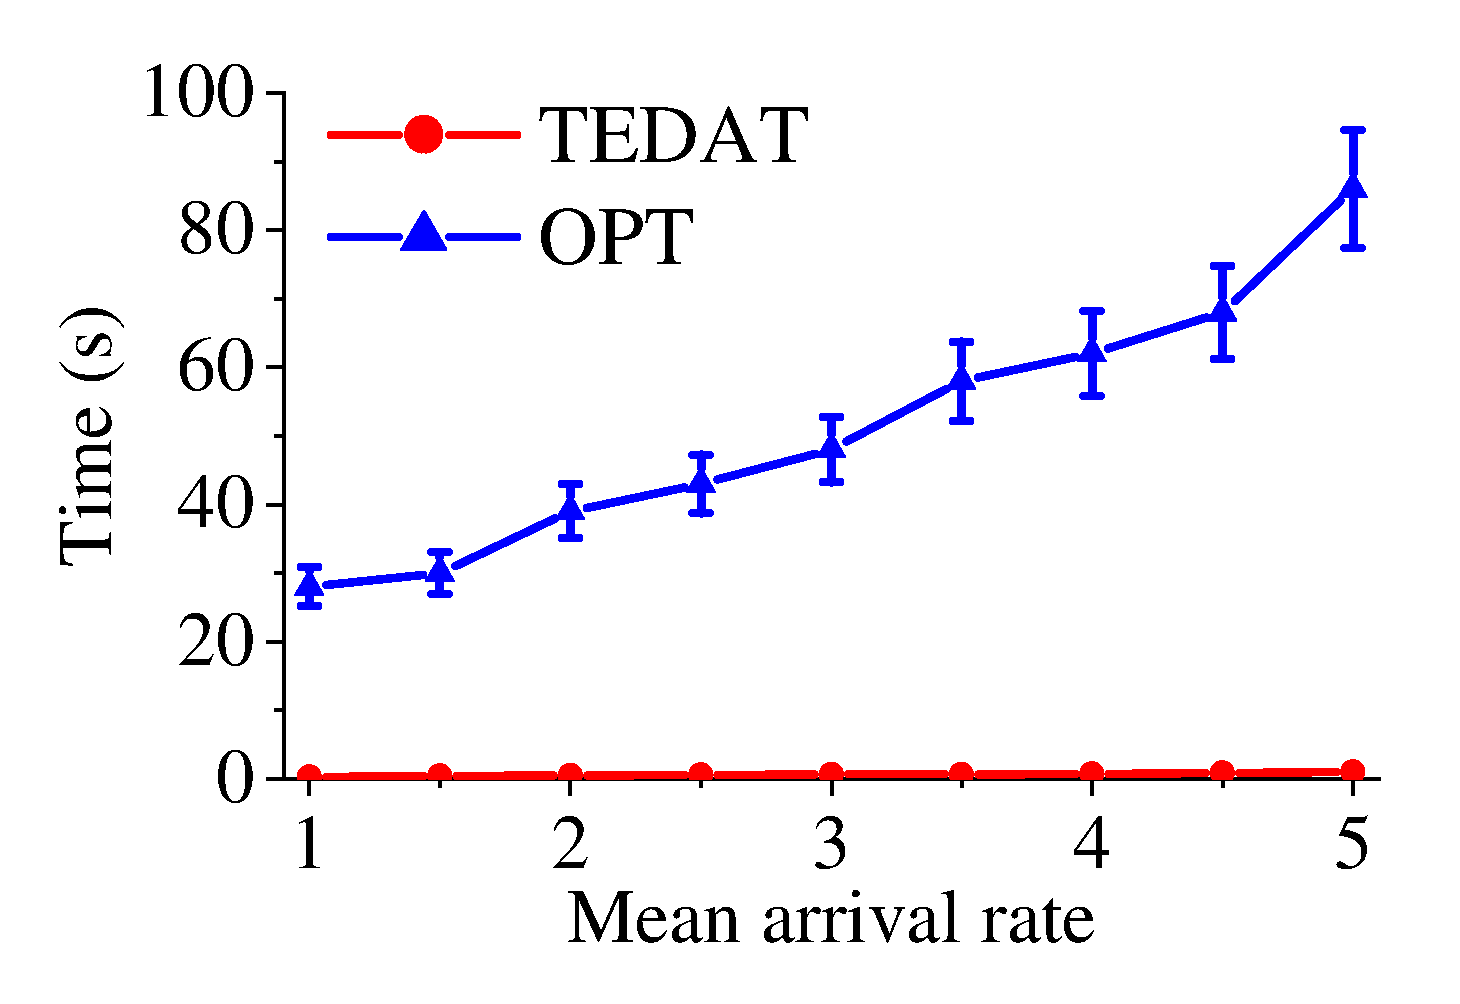
\includegraphics[width=1.8 in]{fig/evaluation/admission-control-time.pdf}
%    \caption{Weight difference.} 
%    \label{fig-weight} 
%  \end{minipage}% 
%%  \begin{minipage}[t]{0.24\linewidth} 
%%    \centering 
%%    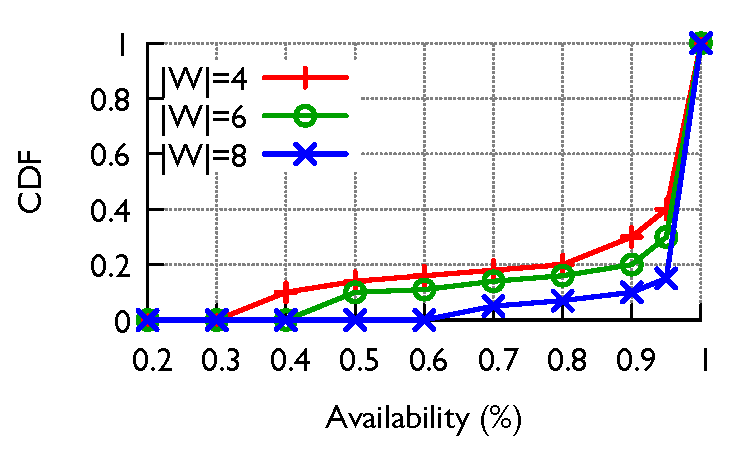
\includegraphics[width=1.7 in]{fig/evaluation/weightnumber.pdf} 
%%    \caption{Important profit.} 
%%    \label{fig-weightnumber} 
%%  \end{minipage}% 
%   \begin{minipage}[t]{0.25\linewidth} 
%    \centering 
%    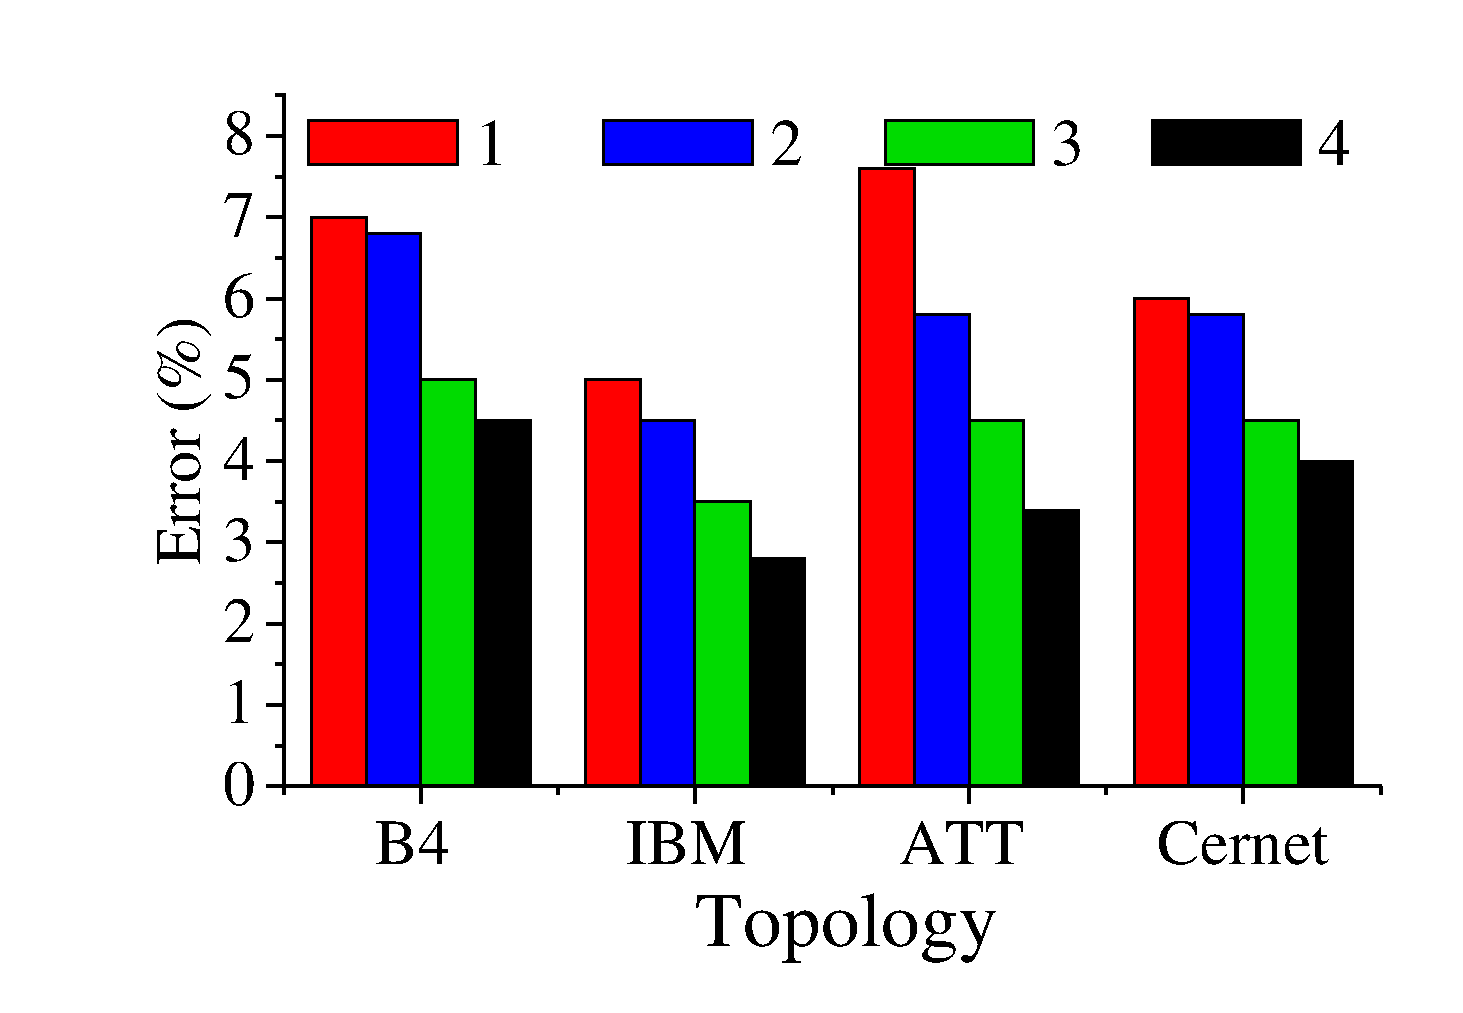
\includegraphics[width=1.8 in]{fig/evaluation/error.pdf}
%    \caption{Weight difference.} 
%    \label{fig-weight} 
%  \end{minipage}% 
%     \begin{minipage}[t]{0.25\linewidth} 
%    \centering 
%    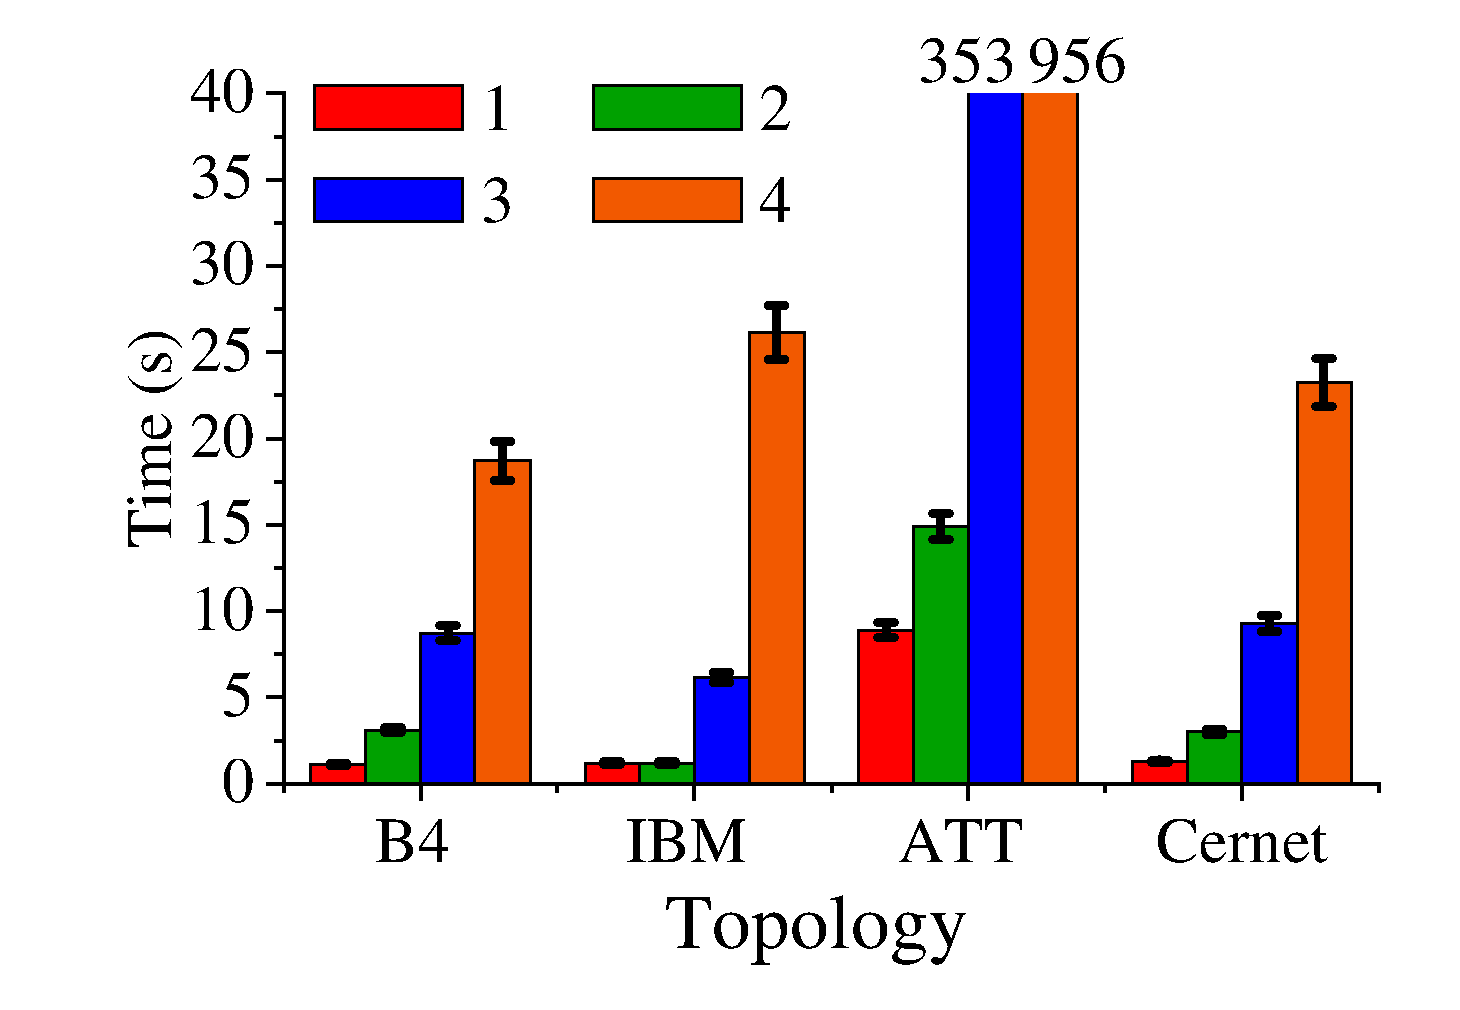
\includegraphics[width=1.8 in]{fig/evaluation/optimization_time.pdf}
%    \caption{Weight difference.} 
%    \label{fig-weight} 
%  \end{minipage}% 
%  
%\end{figure*}

\subsection{Simulation evaluation}
\textbf{Simulation setup.} 
We evaluate the performance of $\mathsf{BATE}$ under four network topologies: B4 \cite{B4}, ATT \cite{Teavar}, IBM\cite{SMORE}, CERNET2 (China Education and Research Network), where the first three topologies (including their traffic metrics) are obtained from the authors of TEAVAR\cite{Teavar} and CERNET2 is measured by ourselves.
Table \ref{evaluation-topologies} shows the topology details.
To accommodate the reproducibility of link failures, we make the assumption that link failures fit Weibull distribution, which has been widely used in studying failures over backbones \cite{Characterization} and inter-DC WAN \cite{Teavar}.
Link failure probability varies each time slot with Weibull distribution.
Each run simulates 150000  1-minute timeslot (about 100 days).
The Weibull distribution probability density function $f(\lambda,k)$ contains two parameters, where $\lambda$ is shape parameter and $k$ is scale parameter.
We choose $f(0.8,0.00001)$ as our default distribution, which is similar to \cite{Teavar}.
Tenants' demands can arrive at anytime.
%After a request arriving the system, we run admitted control algorithm to determine whether the request can be accommodated or not.
%As introduced above, $\mathsf{BATE}$ adopts Algorithm \ref{greedy} as its default option.
%We compare Algorithm \ref{greedy} (i.e, Greedy) with fixed algorithm and the optimal algorithm
%The fixed algorithm assumes all admitted requests are fixed and checks whether the remaining network capacity can support the new request.
%The optimal algorithm determines whether the new request can be admitted by solving (\ref{P8}). 
%Every time slot, we randomly generate an integer $p$ between 0 and 10000 for each link.
%If  $p/10000$ is smaller than the failure probability of the link, we make it down to emulate failure.
%Then after 5 time slots, we make the link up again.
%Each experiment lasts 200 time slots.
%The achieved availability of a service is computed as the percentage of qualified time slots, where a slot is regarded as qualified if the total bandwidth is not smaller than demand.
%The achieved availability can be derived by a post-processing simulation composed by network states.
%In each network state, we record the application level throughput ratio as well as the network state probability.
%The sum of network state probability in which the allocated bandwidth larger than the demand is regarded as the achieved availability.
Traffic engineering performs every 10 time slots.
For traffic engineering part, we compare the performance of $\mathsf{BATE}$ against FFC \cite{FFC}, TEAVAR \cite{Teavar}, SWAN \cite{swan}, SMORE \cite{SMORE}, B4 \cite{B4}.
We change them to adapt service level traffic engineering: 
FFC tries to maximize the link utilization with considering 1 fault could occur in our evaluation.
%To fairly compare the ability of the FFC algorithm, we let it
%send the entire demand at the expense of potential degradation in
%availability, unless otherwise stated
%TEAVAR uses the parameter $\beta$ to control the network service availability target
TEAVAR maximizes bandwidth allocation to each demand subject to a single operator-specified availability target.
The default availability target of TEAVAR is $99.9\%$ in our simulations.
SMORE \cite{SMORE} minimizes the maximum link utilization without explicit guarantees on availability.
SWAN \cite{swan}  tries to  maximize the total throughput of all demands in the current slot.
B4 \cite{B4} aims to deliver max-min fair allocation manner to each demand.
%We compare the failure recovery part with random rerouting mechanism when there are link failures. 
%However, SWAN 
%However, TEAVAR .
%SWAN 
%We can see that DC5 takes about 100ms to detect failure and DC1 hears it within 200ms.
%It takes about 200ms for the controller to derive the new traffic engineering results.
%Switches take about 500ms to update flow rules.
%DC4-DC5 link has large failure probability, so the scenario mentioned above is likely to happen.
%Traditionally,  SDN controller will take reactive interventions when there are failures.
%This will take too much time and QoS might have already been hurt disastrously. 
%This demonstrates that $\mathsf{BATE}$ considers failure scenarios \textit{proactively}.
%Services with large availability target will pass links with low risk probability. 
%Therefore, the availability target can be guaranteed.
%$\mathsf{BATE}$ considers the failure probability of links, thus, the availability demand of applications can be guaranteed.
%\begin{figure*}
%\centering
%\subfigure[Network state coverage]{
%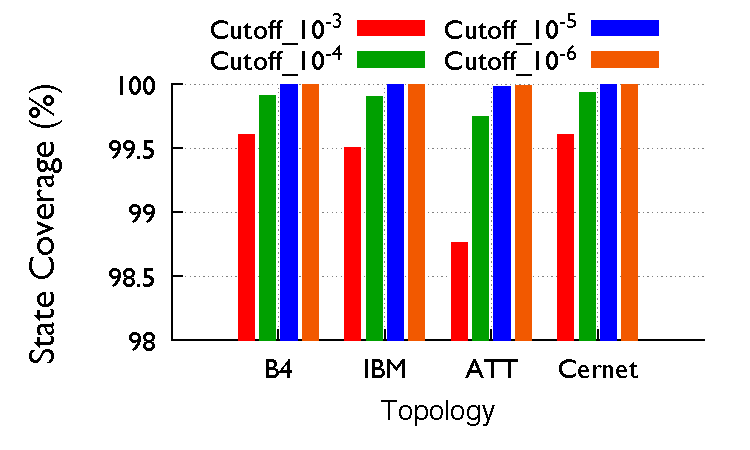
\includegraphics[width=0.32\textwidth]{fig/coverage.pdf}}
%\subfigure[Error]{
%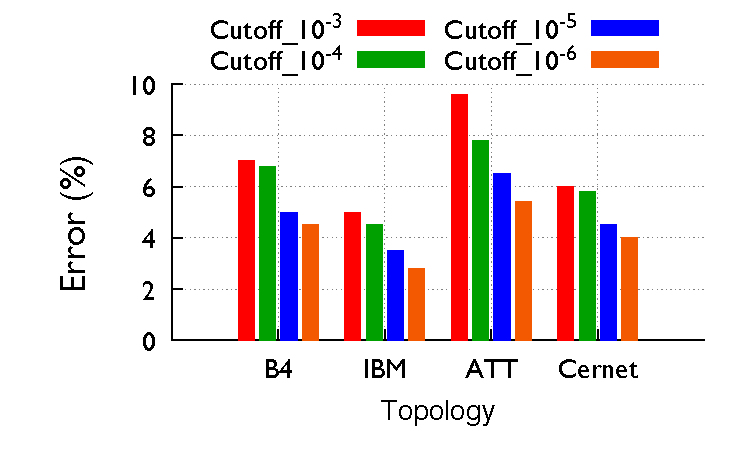
\includegraphics[width=0.32\textwidth]{fig/error.pdf}}
%\subfigure[Solution time]{
%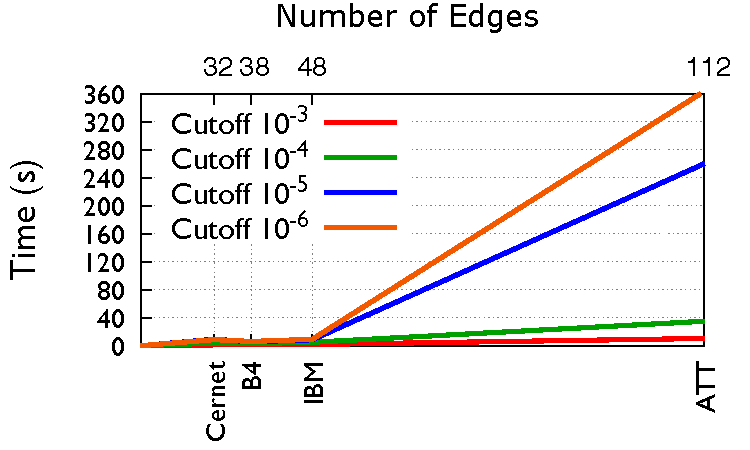
\includegraphics[width=0.32\textwidth]{fig/optimizer_times.pdf}}
%\caption{Impact of pruning and accuracy of solution.}
%\label{purning_fig2}
%\end{figure*}
%As introduced above, $\mathsf{BATE}$ calls for application level volume between each DC pair.
%Our collected traffic data contains the capacity of all links and the  bandwidth demands between each DC pair.
%We don't have real bandwidth demands of each service.
%%We assume there are $|J|=30$ application flows in each DC pair.
%To conform real data center network traffic characters, we divide the original DC-pair bandwidth demands into $|J|$ parts randomly, where the default value of $J$ is 30.
%%Each part can be regarded as an application flow demand.
%Services call for diverse availability demands and we generate them with uniform distribution between 90\% and 99.99\%.  
%There are typically five importance levels in current data centers, i.e., significant,
%important, normal, unimportant and lax.
%We randomly assign weights to services within \{1,2,3,4,5\}with uniform distribution, which is similar to \cite{hanzhang}.
% $\mu(f_{jtk})=\sum_{k\in K, t \in T_k}f_{jtk}/d_j, \forall j \in J$ in our experiments.
%Default  profit is 1 when availability is achieved, otherwise, the profit is $\mu(R_j)=0.01\times R_j$.
We consider 10 availability targets, whose value are from the SLAs of Azure \cite{azure}.
Our collected traffic data contains the capacity of all links.
We generate tenants' bandwidth demands with a Poisson process, the duration of each demand is modeled as an exponential distribution with a mean of 1000 time slots.
%To closely mimic the real traffic matrix, the total bandwidth of generated requests between each node pair equals to that collected from the real traffic matrix.



%\begin{figure*}[t]
%\centering
%%\subfigure[Weight differentiation]{
%%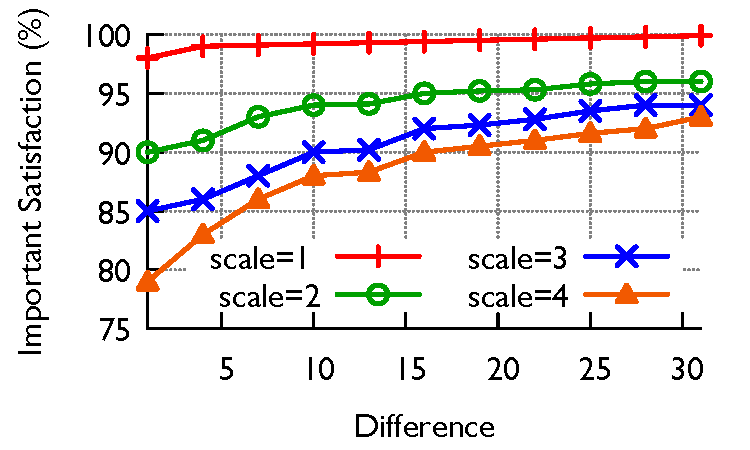
\includegraphics[width=0.32\textwidth]{fig/evaluation/Geometric.pdf}}
%%\subfigure[Solution comparison]{
%%\includegraphics[width=0.32\textwidth]{fig/evaluation/version.pdf}}
%%\subfigure[Tunnel selection]{
%%\includegraphics[width=0.32\textwidth]{fig/evaluation/routing.pdf}}
%\subfigure[Profit comparison]{
%\includegraphics[width=0.32\textwidth]{fig/evaluation/fake/totalprofit.pdf}}
%\subfigure[Target satisfaction percentage]{
%\includegraphics[width=0.32\textwidth]{fig/evaluation/weight.pdf}}
%\subfigure[Availability comparison]{
%\includegraphics[width=0.32\textwidth]{fig/evaluation/fake/availability-cdf.pdf}}
%%\subfigure[Same importance]{
%%\includegraphics[width=0.24\textwidth]{fig/evaluation/sameweight.pdf}}
%\caption{Performance comparison under different metrics with IBM topology and traffic trace.}
%\label{motivatio_fig2}
%\end{figure*}


%\textbf{Metrics}.
%We evaluate a few different metrics.
%Firstly, we examine request acceptance/reject rate of each request admission control scheme.
%Secondly, we compare the requests satisfied availability targets fraction between $\mathsf{BATE}$ and other engineering schemes.
%Thirdly,  we report other related metrics such as network link utilization, admitted bandwidth, achieved availability and computation overhead. 


%SWAN \cite{swan} divides services into three categories and allocates demands in priority order (i.e., background $<$ elastic $<$ interactive).
%For SWAN, we regard the Significant and Important services as interactive ones, Normal services as elastic ones, and the other services as background ones.
%Nowadays, some ISP networks are designed with worst-case assumptions about failures, so topologies might be over-provisioned. 
%%Therefore, we begin with the real input demands and compute the percentage of applications satisfied availability demands.
%Therefore, we scale up the demands by a factor $s$, which is similar to the technology used in \cite{SMORE, FFC, Teavar}.


%\begin{figure*}
%\centering
%%\begin{tabular}{c}
%%\includegraphics[width=0.7\textwidth]{fig/evaluation/legend.pdf}
%%\end{tabular}
%%\vfill
%\subfigure[Total profit ]{
%\includegraphics[width=0.32\textwidth]{fig/evaluation/fake/totalprofit.pdf}}
%\subfigure[Satisfaction fraction details]{
%\includegraphics[width=0.32\textwidth]{fig/evaluation/weight.pdf}}
%\subfigure[Profit details ]{
%\includegraphics[width=0.32\textwidth]{fig/evaluation/weightprofit.pdf}}
%\caption{Availability satisfaction fraction of applications with different importance under IBM topology and traffic, where L, U, N, I, S are abbreviations of Lax, Unimportant, Normal, Important and Significant.}
%\label{availability_fig2}
%\end{figure*}

\subsubsection{Performance under real network topologies}\label{scales}
%From the comparison between the scheduled and testbed results, we can see that the scheduled results match the real testbed quite well,
%so in the following part, we will use trace-driven simulation to evaluate the performance of $\mathsf{BATE}$.




%
%
%
%
%
%
%
% \begin{figure}[h]
%\begin{center}
%\includegraphics [width=0.8\columnwidth] {fig/evaluation/fake/totalprofit.pdf}
%\caption{Profit comparison between $\mathsf{BATE}$ and other Traffic engineering schemes.}
%\label{sim-profit}
%\end{center}
%\end{figure}



%\includegraphics[width=0.32\textwidth]{fig/evaluation/fake/totalprofit.pdf}}








%\begin{figure}[t]
%\begin{center}
%\includegraphics [width=0.9  \columnwidth] {fig/evaluation/fake/availability-cdf.pdf}
%\caption{ $\mathsf{BATE}$ to various TE schemes when network capacity is over-provisioned.}
%\label{sim-importance2}
%\end{center}
%\end{figure}

%\begin{figure}[h]
%\centering
%%\begin{tabular}{c}
%%\includegraphics[width=0.7\textwidth]{fig/evaluation/legend.pdf}
%%\end{tabular}
%\subfigure[Accuracy of greedy algorithm]{
%\includegraphics [width=0.48\columnwidth] {fig/evaluation/link-utilization.pdf}}
%\subfigure[Efficiency comparison]{
%\includegraphics [width=0.48\columnwidth] {fig/evaluation/admission-control-time.pdf}}
%\caption{Error and efficiency comparisons.}
%\label{availability_fig3}
%\end{figure}
%



%\begin{figure}[h]
%\centering
%%\begin{tabular}{c}
%%\includegraphics[width=0.7\textwidth]{fig/evaluation/legend.pdf}
%%\end{tabular}
%%\subfigure[Accuracy of greedy algorithm]{
%%\includegraphics [width=0.48\columnwidth] {fig/evaluation/error.pdf}}
%%\subfigure[Efficiency comparison]{
%%\includegraphics [width=0.48\columnwidth] {fig/evaluation/optimization_time.pdf}}
%%\caption{Error and efficiency comparisons.}
%%\label{availability_fig3}
%%\end{figure}

%
%\begin{figure*} 
%   \begin{minipage}[t]{0.33\linewidth} 
%    \centering 
%    \includegraphics[width=2.4 in] {fig/evaluation/admission-control-time.pdf}}
%    \caption{Weight difference.} 
%    \label{fig-weight} 
%  \end{minipage}% 
%%  \begin{minipage}[t]{0.24\linewidth} 
%%    \centering 
%%    \includegraphics[width=1.7 in]{fig/evaluation/weightnumber.pdf} 
%%    \caption{Important profit.} 
%%    \label{fig-weightnumber} 
%%  \end{minipage}% 
%  \begin{minipage}[t]{0.33\linewidth} 
%    \centering 
%    \includegraphics[width=2.4 in]{fig/evaluation/error.pdf} 
%    \caption{More $\mathsf{BATE}$ versions.} 
%    \label{fig-version} 
%  \end{minipage} 
%   \begin{minipage}[t]{0.33\linewidth} 
%    \centering 
%    \includegraphics[width=2.4 in]{fig/evaluation/optimization_time.pdf}}
%    \caption{More routing schemes.} 
%    \label{routing-version} 
%  \end{minipage} 
%\end{figure*}


%For example, if the bandwidth reservation that is larger than demands in 99.9\% network states, then the sum of the probability for the 99.9\% network states present the achieved availability.
%We care about the following metrics:
%(1) Availability satisfaction fraction. It denotes the percentages of applications whose achieved availability is larger than the corresponding target.
%(2) Total availability profit.  The total availability profit presents the whole performance of the schemes.

Figure \ref{availability_fig1}(a)  shows $\mathsf{BATE}$  rejects only about 3\% more demands than the optimal solution and can accept about 50\% more demands than the \textit{Fixed} consistently.
Similar to \cite{Teavar}, we next start a post-processing simulation, in which intends to send entirely bandwidth under each scenario at each time slot.
%We write down the bandwidth loss of each scenario for each demand and each scenario's corresponding probability.
The sum of scenario probability where demand is fully satisfied reflects the \textit{achieved availability}.
%If a demand's , then the availability defined in SLA is \textit{satisfaction}.
The term \textit{satisfaction percentage} refers to the fraction of total arrival demands whose achieved availability are higher than their availability targets throughout duration.
Figure \ref{availability_fig1}(b) demonstrates that $\mathsf{BATE}$ can make 40\% more demands satisfy SLA availability.
%Demands SLA violation of  $\mathsf{BATE}$ mainly comes from admission control rejection.
%The reason for this is that $\mathsf{BATE}$ adopts admission control and it considers the diverse availability targets of different bandwidth demands.
$\mathsf{BATE}$ can make demands with stringent availability requirements pass links with high reliability, therefore, their availability targets can be guaranteed, but other schemes are unable differentiate demands.
To show this benefit, we adopt \textit{Fixed} admission control for each traffic scheduling algorithm, then Figure \ref{availability_fig1}(c) shows $\mathsf{BATE}$ performs at least 10\% better than other algorithms under the \textit{Fixed} admission control method.
Figure \ref{availability_fig1}(d) shows the average monetary gain percentage for the scenario in which one failure could occur in the network.
We can see $\mathsf{BATE}$  is able to retain 30\% more profit than other algorithms when network fails.
\begin{figure}
\centering
\subfigure[Cutoff error]{
\includegraphics[width=0.23\textwidth]{fig/evaluation/error.pdf}}
\subfigure[Optimization time]{
\includegraphics[width=0.23\textwidth]{fig/evaluation/optimization_time.pdf}}
\caption{Impact of pruning for traffic scheduling.}
\label{availability_fig3}
\end{figure}
We qualify the scalability by measuring the admission control time for each demand.
The simulation is performed on a Linux server (4-core, 2.60GHz processor with 32GB).
As shown in Figure \ref{admission-benefit}, the admission control time of $\mathsf{BATE}$ is less than 1s with about less than 5\% error, which is at least 30$\times$ faster the global optimal solution under ATT topology.
Algorithm \ref{pruning} cuts off the scenarios that can hardly happen.
%Algorithm \ref{pruning} runs in depth-first manner and when the current network state is smaller than the threshold, the remaining state of the search tree can be ignored.
%Figure \ref{purning_fig2} (a) shows the percentage of network state coverage.
%We can see that even with small cutoff threshold, more than 97\% probability are included.
% In Section \ref{solutions}, we show how to derive the solutions for WAPM problem.
% The errors mainly comes from two parts, i.e., ILP approximate algorithm and pruning.
%In Appendix \ref{B}, we analyze the approximation of the greedy heuristic is 2 in an ideal case.
%Algorithm \ref{greedy} proposes a greedy algorithm to solve $\mathsf{BATE}$ problem.
Let $\mathsf{BATE}$ denote the overall achieved availability of all admitted demands with scenario pruning  and $OPT$ denote the achieved availability of optimal solution without scenario pruning. 
Then the error can be defined as $\frac{|\mathsf{BATE} -OPT|}{|OPT|}$.
Figure \ref{availability_fig3} (a) shows the error of pruning algorithm with different current link failure numbers.
We can see the error is less than 8\% even the current link failure number is 1.
Traditionally, TE should update the network state every 5-10 minutes.
% and though the powerful mathematical optimization solver such as Gurobi \cite{gurobi} can solve $\mathsf{BATE}$ problem, it might be too slow.
Figure \ref{availability_fig3} (b) shows the time when solving it with Gurobi \cite{gurobi} on the server (4-core, 2.60GHz processor with 32GB ).
We can see that even on a large network (e.g., ATT topology), at most  15 seconds are needed when current link failure numbers are 2, which is fast enough in reality.
%We can see that for large network (e.g., ATT topology) , Gurobi is too slow to converge and the greedy algorithm is necessary.
%While the bruce force algorithm is more than 1000 minutes for each topology and we don't paint them in the picture.
%We can see the result is fast enough to deploy in practice.
\begin{figure*} 
   \begin{minipage}[t]{0.24\linewidth} 
    \centering 
    \includegraphics[width=1.6 in]{fig/evaluation/routing.pdf}
    \caption{Routings.} 
    \label{routing-version} 
  \end{minipage}% 
   \begin{minipage}[t]{0.24\linewidth} 
    \centering 
    \includegraphics[width=1.6 in]{fig/evaluation/approximation.pdf}
    \caption{Approximation.} 
    \label{approximation} 
  \end{minipage}
     \begin{minipage}[t]{0.24\linewidth} 
    \centering 
    \includegraphics[width=1.6 in]{fig/evaluation/approximation.pdf}
    \caption{Approximation.} 
    \label{approximation} 
  \end{minipage}
       \begin{minipage}[t]{0.24\linewidth} 
    \centering 
    \includegraphics[width=1.6 in]{fig/evaluation/approximation.pdf}
    \caption{Approximation.} 
    \label{approximation} 
  \end{minipage}
  
\end{figure*}

So far, we use K-shortest path as the default tunnel selection scheme.
There are also other tunnel selection schemes, e.g., edge disjoint paths\cite{Bruno2013Dynamic}, oblivious routing\cite{SMORE}.
Figure \ref{routing-version} shows the comparison with different tunnel selection methods.
We can see that (1) $\mathsf{BATE}$ performs well regardless the tunnel selection algorithm.
This indicates that the success of $\mathsf{BATE}$ doesn't reply on the particular routing scheme;
(2)  Oblivious routing is still slighter better than KSP and edge disjoint paths.
This is because it is intended to avoid link over-utilization through diverse and low-stretch path selection.

We propose a greedy for failure recovery optimization problem.
Figure \ref{approximation} shows the approximation of the greedy algorithm, where the approximation can be defined as the profit ratio of optimal solution and greedy solution.
We can see that the profit loss of greedy algorithm is less than 10\%.
%Satisfaction percentage. It denotes the percentages of applications whose achieved availability is larger than the corresponding target.
%Figure \ref{availability_fig1}(b) shows 
%$\mathsf{BATE}$ performs about 20\%, 25\%, 30\%,  40\% better than TEAVAR, SMORE, SWAN, FFC, respectively.
%%Specially, when traffic scale is 3, more than 70\% applications can satisfy their availability demands, which is at least 30\% better than TEAVAR.
%Specially, the advantage of $\mathsf{BATE}$  is more obvious when there are resource competition (e.g., $s=3$).
%%The reason for this is that $\mathsf{BATE}$ considers the bandwidth-based availability demand differentiation of applications.
%This picture also demonstrates that the performance of $\mathsf{BATE}$ doesn't depend on particular network topology and traffic.
%Next, we take IBM trace as the example and perform the experiments.

 
%Figure \ref{motivatio_fig2}(a) shows total profit comparison between $\mathsf{BATE}$ and other schemes.
%We can see that   $\mathsf{BATE}$ performs best and its performance is even up to 30\%, 40\%, 50\%, 75\% better than TEAVAR, SMORE, SWAN and FFC when traffic scale is 3.
%Figure \ref{motivatio_fig2}(b) shows the percentage of services whose availability targets are satisfied for different importance levels when traffic scale is 3. 
%In the picture, L, U, N, I, S are abbreviations of Lax, Unimportant, Normal, Important and Significant, and the error bar paints the mean
%and mean $\pm$ standard deviation value.
%We can see $\mathsf{BATE}$ performs even worse than other TE schemes for the Lax services, but it performs at least 25\% better for the Important and Significant services.
%%We can see that  40\% more important services (i.e., Important, Significant) under $\mathsf{BATE}$ can meet their availability demands.
%%,since the importance of services is taken into consideration under  $\mathsf{BATE}$, while most schemes ignore this.
%Specially, we can see that SWAN \cite{swan} also performs well for the importance services, but it allocates bandwidth only in strict precedence across  three coarse priority classes and  $\mathsf{BATE}$ is  fine-grained priority and can describe the five level of importance.
% $\mathsf{BATE}$ aims to maximize the sum profit of all services, where a service's profit is defined in (\ref{availability}).
%Figure \ref{motivatio_fig2}(c) presents the CDF of achieved availability for different schemes when traffic scale is 3.
%We can see that about 87\%  services's achieved availability are larger than 95\% under  $\mathsf{BATE}$, which is at least 30\% better than other schemes.
%Figure \ref{motivatio_fig2}(a) shows that larger tunnel number can provide slighter higher availability.
%This is because that more alternative tunnels can be used to meet the bandwidth demands.
%Our trace doesn't contain application level traffic matrix, so we divide the original WAN traffic into $|J|=30$ parts randomly.
%Figure \ref{motivatio_fig2}(b) demonstrates the performance with more application division.
%We can see the performance is consistent for various application number.
%





%Figure \ref{availability_fig2} shows availability satisfaction fraction of applications with different importance.
%Figure \ref{availability_fig2}(a) demonstrates the total profit.
%We can see that $\mathsf{BATE}$ gains more 20\% profit than other schemes.
%The reason for this is that more applications under $\mathsf{BATE}$ could meet their availability demands.
%Figure \ref{availability_fig2}(b) and Figure \ref{availability_fig2}(c) show the satisfaction fraction and profit details for applications with different level of importance.


%We use 5-levels to present the importance of applications and we have test the differentiation between the adjacent level.
%In reality, more important levels might be needed to satisfy the user demands.
%Figure \ref{motivatio_fig2}(c) shows the performance with different level number.
%We can see both profit and satisfaction fraction are stale regardless the number of levels.




%In WAN network, the failure probability of a single link differs even by 1000 times.



%\textbf{Path selection.}
%
%
% \begin{figure}
%\begin{center}
%\includegraphics [width=0.8\columnwidth] {fig/evaluation/routing.pdf}
%\caption{Effect of link utilization. }
%\label{routing}
%\end{center}
%\end{figure}




%\begin{figure}
%        \centering
%        \begin{tabular}{c}
%\includegraphics[width=0.45\textwidth]{fig/evaluation/legend2.pdf}
%\end{tabular}  
%       \subfigure[Whole network]{
%         \includegraphics [width=0.23 \textwidth] {fig/topologyutilization.pdf}}
%       \subfigure[Low failure probability]{
%        \includegraphics[width=0.23\textwidth]{fig/topologyutilization2.pdf}}
%     \caption{Link utilization comparison}
%    \label{topologyutilization}
%\end{figure}




%\subsubsection{Performance under different settings}\label{settings}
%%We now evaluate the performance of $\mathsf{BATE}$ under different settings with  IBM topology and trace.
%
%\textbf{Magnitude of weights.}
%In the previous experiments, we set weight within \{1,2,3,4,5\} to present the importance of services. 
%In this part, we evaluate the performance with different magnitude of weights.
%Figure \ref{fig-weight} shows the satisfaction fraction for the Important and Significant services under $\mathsf{BATE}$, when weight difference between the adjacent levels ranges from 1 to 32 (e.g., if the difference is 2, weight set is \{1,3,5,7,9\}).
%We can see that the satisfaction fraction becomes steady after increasing.
%This is because when heightening weight gap,  important services can gain more resources and meet their availability targets with high probability.
%
%%\textbf{Weight number.}
%%Five important levels are used in the experiments shown above.
%%Figure \ref{fig-weightnumber} shows the profit cumulative distribution for important applications (tail 20\%).
%%We can see that more than 80\% important applications achieve their availability targets. 
%%Specially, more important levels can benefit  those important applications.
%
%\textbf{More $\mathsf{BATE}$ solutions.}
%%The default  profit is 1 for applications whose availability demands are satisfied, otherwise the profit is $\mu(R_j)=0.01\times R_j$.
%We denote the $\mathsf{BATE}$ version used in the previous experiment as $\mathsf{BATE}$-A.
%We now define $\mathsf{BATE}$-B, whose gained profit is 1 for $S_j\ge \beta_j$ and 0.75 for other cases.
%$\mathsf{BATE}$-C's gained profit  is 1 for $S_j\ge \beta_j$ and $\mu(f_{jtk})=1-(\beta_j-S_j)$.
%Figure \ref{fig-version} shows the performance comparison for the three schemes.
%We can see that the performance gap between the three algorithms is narrow: less than 5\%.
%This demonstrates $\mathsf{BATE}$ is a general framework that does not depend on the particular profit function.
%
%\textbf{Various routing schemes.}
%So far, we use K-shortest path as the default tunnel selection scheme.
%There are also other tunnel selection schemes, e.g., edge disjoint paths\cite{Bruno2013Dynamic}, oblivious routing\cite{SMORE}.
%Figure \ref{routing-version} shows the comparison with different tunnel selection methods.
%We can see that (1) $\mathsf{BATE}$ performs well regardless the tunnel selection algorithm.
%This indicates that the success of $\mathsf{BATE}$ doesn't reply on the particular routing scheme;
%(2)  Oblivious routing is still slighter better than KSP and edge disjoint paths.
%This is because it is intended to avoid link over-utilization through diverse and low-stretch path selection.
%
%
%\textbf{Link failure probability standard deviation.}
%Weibull distribution is used to generate link failure probability in our simulations.
%Figure \ref{sim-importance2} presents profit comparison under different link failure probability standard deviation.
%We can see that $\mathsf{BATE}$ and TEAVAR perform better under higher link failure probability standard deviation.
%The reason for this is that they both consider link failure probability in their TE formulation. 
%%We can see that all schemes degrade with higher failure probability, but $\mathsf{BATE}$ still performs at least 15\% better than other schemes.
%%Specially, FFC has the smallest influence, since its bandwidth allocation considering at one link failure beforehand.
%
%
%
%
%
%
%
%
%
%
%
%\subsubsection{Solution accuracy}\label{purning}
%Solution error mainly comes from scenario pruning and greedy heuristic algorithm.






\section{Related work}\label{relate}

\textbf{Traffic engineering for WAN.}
Optimizing WAN performance is a big challenge.
Prior technologies such as OSPF\cite{OSPF} and MPLS tunnels \cite{MATE,Tightrope} can improve the backbone traffic transfer under the knowledge of traffic demands.
Recently, SDN is widely used in WAN TE.
SWAN\cite{swan}, B4\cite{B4,hong2018b4}, Bwe\cite{bwe},OWAN\cite{OWAN} leverage the whole network information to allocate network bandwidth.
Network scheduling schemes \cite{calendaring,dynamic,D3} also use SDN technology to decide the priority of traffic.
Although these schemes can improve the network utilization, they ignore the \textit{risk} of networks, thus, service availability can't be guaranteed.
%\cite{,evole,Teavar,,FFC,,dynamic,SMORE,,OWAN}.  

\textbf{Network risk based traffic engineering.}
\cite{evole} studies the network failures and proposes the principles to design robust network, but it doesn't contain any TE framework.
\cite{Optical} suggests that backbone traffic engineering strategies should consider current and past optical layer performance.
Neither \cite{evole} nor \cite{Optical} contains TE frameworks.
 \cite{Stochastic} models demand and risks as uncertainty, but it can't provide availability at the particular level (e.g., 90\%).
 \cite{bi2019uncertainty-aware} can adjust traffic according to demands, but it ignores the link failures.
 Most of the traffic engineering schemes work in the \textit{reactive} manner, such as \cite{jointfailure},\cite{R3}.
The reactive methods could take a long time to recover from faults, while applications have already been hurt\cite{FFC}.
FFC \cite{FFC} and TEAVAR\cite{Teavar} are proactive routing protection methods, but they can't ensure the resources of services under network failures.
%In this case, FFC \cite{FFC} advocates to take link failure into consideration when allocating network resources.
%Traffic are freedom from congestion under arbitrary combinations of up to $k$ faults with FFC.
%However, FFC will lead to low link utilization.
%To relieve this, TEAVAR\cite{Teavar} considers the probability of link failure and tries to maximize link utilization under the particular availability target.
%Although TEAVAR tries to fully utilize the link capacity, it ignores the availability difference of applications.
%Moreover, both FFC and TEAVAR uses connectivity-based availability, which can't ensure the resources of applications under network failures.
$\mathsf{BATE}$ makes a further step and tries to provide service level bandwidth-based availability.
The availability of $\mathsf{BATE}$ is stronger than them.



\textbf{Bandwidth guarantee.}
Up still now, many existing works have already considered to guarantee the bandwidth of applications over inter or intra DCs.
Deadline-aware schemes such as D$^2$TCP\cite{D2TCP}, LPD \cite{LPD}, Amoeba\cite{Guaranteeings}  try to make flows finish before a fixed time constraints,
but they can't perform finely grained rate limits.
Some cloud bandwidth limit technologies such as CloudMirror \cite{appdriven} and EyeQ \cite{EyeQ}, can provide bandwidth guarantees to applications or tenants, while they ignore the network risks and service availability requirements.
$\mathsf{BATE}$ is different from in two aspects.
Firstly, $\mathsf{BATE}$ considers the network failures and tries to perform rate limit under the assumption.
Secondly, $\mathsf{BATE}$ can guarantee bandwidth at a particular level (e.g., 99\%). 

%\begin{figure}[t]
%\begin{center}
%\includegraphics [width=0.9\columnwidth] {fig/evaluation/error.pdf}
%\caption{Total profits comparison.}
%\label{sim-error}
%\end{center}
%\end{figure}
\section{Conclusion Remarks}
We present $\mathsf{BATE}$, a framework that attempts to guarantee the availability demands of applications.
 $\mathsf{BATE}$ aims to optimize the total profits of service subject availability targets.
We design greedy and network scenario pruning algorithm to derive the solution.
We evaluate the performance of $\mathsf{BATE}$ in real testbed as well as trace-driven simulations.
The evaluation results demonstrate that $\mathsf{BATE}$ can improve  bandwidth-based availability performance by up to 50\%.







\begin{filecontents}{\jobname.bib}

@article{lamport1998the,
title={The part-time parliament},
author={Lamport, Leslie},
journal={ACM Transactions on Computer Systems},
volume={16},
number={2},
pages={133--169},
year={1998}}
    
    
@inproceedings{ARMA, author = {Bagnall, A. J. and Janacek, G. J.}, title = {Clustering Time Series from ARMA Models with Clipped Data}, year = {2004}, isbn = {1581138881}, publisher = {Association for Computing Machinery}, address = {New York, NY, USA}, url = {https://doi.org/10.1145/1014052.1014061}, doi = {10.1145/1014052.1014061}, booktitle = {Proceedings of the Tenth ACM SIGKDD International Conference on Knowledge Discovery and Data Mining}, pages = {49-58}, numpages = {10}, keywords = {clustering, time series, ARMA}, location = {Seattle, WA, USA}, series = {KDD '04} }


@inproceedings{Guaranteeings, author = {Zhang, Hong and Chen, Kai and Bai, Wei and Han, Dongsu and Tian, Chen and Wang, Hao and Guan, Haibing and Zhang, Ming}, title = {Guaranteeing Deadlines for Inter-Datacenter Transfers}, year = {2015}, isbn = {9781450332385}, publisher = {Association for Computing Machinery}, address = {New York, NY, USA}, url = {https://doi.org/10.1145/2741948.2741957}, doi = {10.1145/2741948.2741957}, booktitle = {Proceedings of the Tenth European Conference on Computer Systems}, articleno = {20}, numpages = {14}, location = {Bordeaux, France}, series = {EuroSys '15} }


@INPROCEEDINGS{LPD,
  author={H. {Zhang} and X. {Shi} and X. {Yin} and F. {Ren} and Z. {Wang}},
  booktitle={2015 IEEE Conference on Computer Communications (INFOCOM)}, 
  title={More load, more differentiation-- A design principle for deadline-aware congestion control}, 
  year={2015},
  volume={},
  number={},
  pages={127-135},}
  
  
@inproceedings {EyeQ,
author = {Vimalkumar Jeyakumar and Mohammad Alizadeh and David Mazi{\`e}res and Balaji Prabhakar and Albert Greenberg and Changhoon Kim},
title = {EyeQ: Practical Network Performance Isolation at the Edge},
booktitle = {Presented as part of the 10th {USENIX} Symposium on Networked Systems Design and Implementation ({NSDI} 13)},
year = {2013},
isbn = {978-1-931971-00-3},
address = {Lombard, IL},
pages = {297--311},
url = {https://www.usenix.org/conference/nsdi13/technical-sessions/presentation/jeyakumar},
publisher = {{USENIX}},
}
@article{D2TCP, author = {Vamanan, Balajee and Hasan, Jahangir and Vijaykumar, T.N.}, title = {Deadline-Aware Datacenter Tcp (D2TCP)}, year = {2012}, issue_date = {October 2012}, publisher = {Association for Computing Machinery}, address = {New York, NY, USA}, volume = {42}, number = {4}, issn = {0146-4833}, url = {https://doi.org/10.1145/2377677.2377709}, doi = {10.1145/2377677.2377709}, journal = {SIGCOMM Comput. Commun. Rev.}, month = aug, pages = {115-126}, numpages = {12}, keywords = {ecn, datacenter, oldi, tcp, deadline, cloud services, sla} }



@inproceedings{R3, author = {Wang, Ye and Wang, Hao and Mahimkar, Ajay and Alimi, Richard and Zhang, Yin and Qiu, Lili and Yang, Yang Richard}, title = {R3: Resilient Routing Reconfiguration}, year = {2010}, isbn = {9781450302012}, publisher = {ACM}, address = {New York, NY, USA}, url = {https://doi.org/10.1145/1851182.1851218}, doi = {10.1145/1851182.1851218}, booktitle = {Proceedings of the ACM SIGCOMM 2010 Conference}, pages = {291-302}, numpages = {12}, keywords = {routing, routing protection, network resiliency}, location = {New Delhi, India}, series = {SIGCOMM '10} }






@article{bi2019uncertainty-aware,
title={Uncertainty-Aware optimization for Network Provisioning and Routing},
author={Bi, Yingjie and Tang, Ao},
pages={1--6},
year={2019}}
    
    
    
@article{Stochastic, author = {Mitra, Debasis and Wang, Qiong}, title = {Stochastic Traffic Engineering for Demand Uncertainty and Risk-Aware Network Revenue Management}, year = {2005}, issue_date = {April 2005}, publisher = {IEEE Press}, volume = {13}, number = {2}, issn = {1063-6692}, url = {https://doi.org/10.1109/TNET.2005.845527}, doi = {10.1109/TNET.2005.845527}, journal = {IEEE/ACM Trans. Netw.}, month = apr, pages = {221-233}, numpages = {13}, keywords = {risk, economics, traffic engineering, mathematical programming, demand uncertainty} }


@inproceedings{Optical, author = {Ghobadi, Monia and Mahajan, Ratul}, title = {Optical Layer Failures in a Large Backbone}, year = {2016}, isbn = {9781450345262}, publisher = {ACM}, address = {New York, NY, USA}, url = {https://doi.org/10.1145/2987443.2987483}, doi = {10.1145/2987443.2987483}, booktitle = {Proceedings of the 2016 Internet Measurement Conference}, pages = {461-467}, numpages = {7}, keywords = {wide-area backbone network, optical layer, outage, availability, q-factor}, location = {Santa Monica, California, USA}, series = {IMC '16} }



@ARTICLE{OSPF,
  author={B. {Fortz} and M. {Thorup}},
  journal={IEEE Journal on Selected Areas in Communications}, 
  title={Optimizing OSPF/IS-IS weights in a changing world}, 
  year={2002},
  volume={20},
  number={4},
  pages={756-767},}
  
  
@INPROCEEDINGS{MATE,
  author={A. {Elwalid} and C. {Jin} and S. {Low} and I. {Widjaja}},
  booktitle={Proceedings IEEE INFOCOM 2001. Conference on Computer Communications. Twentieth Annual Joint Conference of the IEEE Computer and Communications Society (Cat. No.01CH37213)}, 
  title={MATE: MPLS adaptive traffic engineering}, 
  year={2001},
  volume={3},
  number={},
  pages={1300-1309 vol.3},}
  
  @inproceedings{Tightrope, author = {Kandula, Srikanth and Katabi, Dina and Davie, Bruce and Charny, Anna}, title = {Walking the Tightrope: Responsive yet Stable Traffic Engineering}, year = {2005}, isbn = {1595930094}, publisher = {ACM}, address = {New York, NY, USA}, url = {https://doi.org/10.1145/1080091.1080122}, doi = {10.1145/1080091.1080122}, booktitle = {Proceedings of the 2005 Conference on Applications, Technologies, Architectures, and Protocols for Computer Communications}, pages = {253-264}, numpages = {12}, keywords = {distributed, online, responsive, TeXCP, traffic engineering, stable}, location = {Philadelphia, Pennsylvania, USA}, series = {SIGCOMM '05} }
  
  
  
@inproceedings{swan,
author    = {Chi{-}Yao Hong and Srikanth Kandula and  Ratul Mahajan and  Ming Zhang and Vijay Gill and Mohan Nanduri and Roger Wattenhofer},
title     = {Achieving high utilization with software-driven {WAN}},
year = {2013},
booktitle = {{ACM} {SIGCOMM} 2013 Conference, SIGCOMM'13, Hong Kong, China, August 12-16, 2013}
}


@inproceedings{hong2018b4, author = {Hong, Chi-Yao and Mandal, Subhasree and Al-Fares, Mohammad and Zhu, Min and Alimi, Richard and B., Kondapa Naidu and Bhagat, Chandan and Jain, Sourabh and Kaimal, Jay and Liang, Shiyu and Mendelev, Kirill and Padgett, Steve and Rabe, Faro and Ray, Saikat and Tewari, Malveeka and Tierney, Matt and Zahn, Monika and Zolla, Jonathan and Ong, Joon and Vahdat, Amin}, title = {B4 and after: Managing Hierarchy, Partitioning, and Asymmetry for Availability and Scale in Google's Software-Defined WAN}, year = {2018}, isbn = {9781450355674}, publisher = {ACM}, address = {New York, NY, USA}, url = {https://doi.org/10.1145/3230543.3230545}, doi = {10.1145/3230543.3230545}, booktitle = {Proceedings of the 2018 Conference of the ACM Special Interest Group on Data Communication}, pages = {74-87}, numpages = {14}, keywords = {traffic engineering, software-defined WAN}, location = {Budapest, Hungary}, series = {SIGCOMM '18} }

@article{cloudcost, author = {Greenberg, Albert and Hamilton, James and Maltz, David A. and Patel, Parveen}, title = {The Cost of a Cloud: Research Problems in Data Center Networks}, year = {2009}, issue_date = {January 2009}, publisher = {ACM}, address = {New York, NY, USA}, volume = {39}, number = {1}, issn = {0146-4833}, url = {https://doi.org/10.1145/1496091.1496103}, doi = {10.1145/1496091.1496103}, journal = {SIGCOMM Comput. Commun. Rev.}, month = dec, pages = {68-73}, numpages = {6}, keywords = {cloud-service data centers, costs, network challenges} }


@inproceedings{evole,
 author = {Govindan, Ramesh and Minei, Ina and Kallahalla, Mahesh and Koley, Bikash and Vahdat, Amin}, 
 title = {Evolve or Die: High-Availability Design Principles Drawn from Googles Network Infrastructure}, 
 year = {2016},  
 booktitle = {Proceedings of the 2016 ACM SIGCOMM Conference}, 
 series = {SIGCOMM '16} }

@inproceedings{Teavar,
 author = {Bogle, Jeremy and Bhatia, Nikhil and Ghobadi, Manya and Menache, Ishai and Bj\o{}rner, Nikolaj and Valadarsky, Asaf and Schapira, Michael}, title = {TEAVAR: Striking the Right Utilization-Availability Balance in WAN Traffic Engineering}, year = {2019}, isbn = {9781450359566}, publisher = {ACM}, address = {New York, NY, USA}, url = {https://doi.org/10.1145/3341302.3342069}, doi = {10.1145/3341302.3342069}, booktitle = {Proceedings of the ACM Special Interest Group on Data Communication}, pages = {29-43}, numpages = {15}, keywords = {availability, utilization, traffic engineering, network optimization}, location = {Beijing, China}, series = {SIGCOMM '19} }


 
 
@inproceedings{calendaring, author = {Kandula, Srikanth and Menache, Ishai and Schwartz, Roy and Babbula, Spandana Raj}, title = {Calendaring for Wide Area Networks}, year = {2014}, isbn = {9781450328364}, publisher = {ACM}, address = {New York, NY, USA}, url = {https://doi.org/10.1145/2619239.2626336}, doi = {10.1145/2619239.2626336}, booktitle = {Proceedings of the 2014 ACM Conference on SIGCOMM}, pages = {515-526}, numpages = {12}, keywords = {mixed packing covering, deadlines, software-defined networking, wide area network, online temporal planning, inter-datacenter}, location = {Chicago, Illinois, USA}, series = {SIGCOMM '14} }

@inproceedings{FFC, author = {Liu, Hongqiang Harry and Kandula, Srikanth and Mahajan, Ratul and Zhang, Ming and Gelernter, David}, title = {Traffic Engineering with Forward Fault Correction}, year = {2014}, isbn = {9781450328364}, publisher = {ACM}, address = {New York, NY, USA}, url = {https://doi.org/10.1145/2619239.2626314}, doi = {10.1145/2619239.2626314}, booktitle = {Proceedings of the 2014 ACM Conference on SIGCOMM}, pages = {527-538}, numpages = {12}, keywords = {congestion-free, traffic engineering, fault tolerance}, location = {Chicago, Illinois, USA}, series = {SIGCOMM '14} }

@inproceedings{bwe, author = {Kumar, Alok and Jain, Sushant and Naik, Uday and Raghuraman, Anand and Kasinadhuni, Nikhil and Zermeno, Enrique Cauich and Gunn, C. Stephen and Ai, Jing and Carlin, Bj\"{o}rn and Amarandei-Stavila, Mihai and Robin, Mathieu and Siganporia, Aspi and Stuart, Stephen and Vahdat, Amin}, title = {BwE: Flexible, Hierarchical Bandwidth Allocation for WAN Distributed Computing}, year = {2015}, isbn = {9781450335423}, publisher = {ACM}, address = {New York, NY, USA}, url = {https://doi.org/10.1145/2785956.2787478}, doi = {10.1145/2785956.2787478}, booktitle = {Proceedings of the 2015 ACM Conference on Special Interest Group on Data Communication}, pages = {1-14}, numpages = {14}, keywords = {software-defined network, wide-area networks, max-min fair, bandwidth allocation}, location = {London, United Kingdom}, series = {SIGCOMM '15} }

@inproceedings{dynamic, author = {Jalaparti, Virajith and Bliznets, Ivan and Kandula, Srikanth and Lucier, Brendan and Menache, Ishai}, title = {Dynamic Pricing and Traffic Engineering for Timely Inter-Datacenter Transfers}, year = {2016}, isbn = {9781450341936}, publisher = {ACM}, address = {New York, NY, USA}, url = {https://doi.org/10.1145/2934872.2934893}, doi = {10.1145/2934872.2934893}, booktitle = {Proceedings of the 2016 ACM SIGCOMM Conference}, pages = {73-86}, numpages = {14}, keywords = {Inter-datacenter networks;, percentile pricing;, deadline scheduling, dynamic pricing;}, location = {Florianopolis, Brazil}, series = {SIGCOMM '16} }

@inproceedings {SMORE,
author = {Praveen Kumar and Yang Yuan and Chris Yu and Nate Foster and Robert Kleinberg and Petr Lapukhov and Chiun Lin Lim and Robert Soul{\'e}},
title = {Semi-Oblivious Traffic Engineering: The Road Not Taken},
booktitle = {15th {USENIX} Symposium on Networked Systems Design and Implementation ({NSDI} 18)},
year = {2018},
isbn = {978-1-939133-01-4},
address = {Renton, WA},
pages = {157--170},
url = {https://www.usenix.org/conference/nsdi18/presentation/kumar},
publisher = {{USENIX} Association},
month = apr,
}


@inproceedings{B4, author = {Jain, Sushant and Kumar, Alok and Mandal, Subhasree and Ong, Joon and Poutievski, Leon and Singh, Arjun and Venkata, Subbaiah and Wanderer, Jim and Zhou, Junlan and Zhu, Min and Zolla, Jon and H\"{o}lzle, Urs and Stuart, Stephen and Vahdat, Amin}, title = {B4: Experience with a Globally-Deployed Software Defined Wan}, year = {2013}, isbn = {9781450320566}, publisher = {ACM}, address = {New York, NY, USA}, url = {https://doi.org/10.1145/2486001.2486019}, doi = {10.1145/2486001.2486019}, booktitle = {Proceedings of the ACM SIGCOMM 2013 Conference on SIGCOMM}, pages = {3-14}, numpages = {12}, keywords = {wide-area networks, openflow, centralized traffic engineering, routing, software- defined networking}, location = {Hong Kong, China}, series = {SIGCOMM '13} }
 
@inproceedings{OWAN, author = {Jin, Xin and Li, Yiran and Wei, Da and Li, Siming and Gao, Jie and Xu, Lei and Li, Guangzhi and Xu, Wei and Rexford, Jennifer}, title = {Optimizing Bulk Transfers with Software-Defined Optical WAN}, year = {2016}, isbn = {9781450341936}, publisher = {ACM}, address = {New York, NY, USA}, url = {https://doi.org/10.1145/2934872.2934904}, doi = {10.1145/2934872.2934904}, booktitle = {Proceedings of the 2016 ACM SIGCOMM Conference}, pages = {87-100}, numpages = {14}, keywords = {bulk transfers, Software-defined networking, wide area networks, optical networks, cross-layer network management}, location = {Florianopolis, Brazil}, series = {SIGCOMM '16} }

@ARTICLE{cui,  author={Z. {Yang} and Y. {Cui} and X. {Wang} and Y. {Liu} and M. {Li} and S. {Xiao} and C. {Li}},  journal={IEEE/ACM Transactions on Networking},   title={Cost-Efficient Scheduling of Bulk Transfers in Inter-Datacenter WANs},   year={2019},  volume={27},  number={5},  pages={1973-1986},}

@inproceedings{appdriven, author = {Lee, Jeongkeun and Turner, Yoshio and Lee, Myungjin and Popa, Lucian and Banerjee, Sujata and Kang, Joon-Myung and Sharma, Puneet}, title = {Application-Driven Bandwidth Guarantees in Datacenters}, year = {2014}, isbn = {9781450328364}, publisher = {ACM}, address = {New York, NY, USA}, url = {https://doi.org/10.1145/2619239.2626326}, doi = {10.1145/2619239.2626326}, booktitle = {Proceedings of the 2014 ACM Conference on SIGCOMM}, pages = {467-478}, numpages = {12}, keywords = {availability, virtual network, datacenter, application, bandwidth, cloud}, location = {Chicago, Illinois, USA}, series = {SIGCOMM '14} }

@article{tail, author = {Dean, Jeffrey and Barroso, Luiz Andr\'{e}}, title = {The Tail at Scale}, year = {2013}, issue_date = {February 2013}, publisher = {ACM}, address = {New York, NY, USA}, volume = {56}, number = {2}, issn = {0001-0782}, url = {https://doi.org/10.1145/2408776.2408794}, doi = {10.1145/2408776.2408794}, journal = {Commun. ACM}, month = feb, pages = {74-80}, numpages = {7} }


@inproceedings{riskbased, author = {Alipourfard, Omid and Gao, Jiaqi and Koenig, Jeremie and Harshaw, Chris and Vahdat, Amin and Yu, Minlan}, title = {Risk Based Planning of Network Changes in Evolving Data Centers}, year = {2019}, isbn = {9781450368735}, publisher = {ACM}, address = {New York, NY, USA}, url = {https://doi.org/10.1145/3341301.3359664}, doi = {10.1145/3341301.3359664}, booktitle = {Proceedings of the 27th ACM Symposium on Operating Systems Principles}, pages = {414-429}, numpages = {16}, keywords = {network change planning, network compression, network simulations}, location = {Huntsville, Ontario, Canada}, series = {SOSP '19} }

@inproceedings{analysis-osdi, author = {Alquraan, Ahmed and Takruri, Hatem and Alfatafta, Mohammed and Al-Kiswany, Samer}, title = {An Analysis of Network-Partitioning Failures in Cloud Systems}, year = {2018}, isbn = {9781931971478}, publisher = {USENIX Association}, address = {USA}, booktitle = {Proceedings of the 12th USENIX Conference on Operating Systems Design and Implementation}, pages = {51-68}, numpages = {18}, location = {Carlsbad, CA, USA}, series = {OSDI'18} }
@Misc{Cato, year = 2020, author = {{cato}}, title = {Cato Managed Services}, howpublished = {\url{https://www.catonetworks.com}}}
@Misc{Aryaka, year = 2020, author = {{aryaka}}, title = {Aryaka Private WAN}, howpublished = {\url{https://www.aryaka.com}}}

@Misc{amazon, year = 2019, author = {{Amazon}}, title = {Amazon Compute Service Level Agreement (2019)}, howpublished = {\url{https://aws.amazon.com/compute/sla/}}}
@Misc{azure, year = 2020, author = {{Azure}}, title = {Microsoft Azure Service Level Agreements (2020)}, howpublished = {\url{https://azure.microsoft.com/en-us/support/legal/sla/summary/}}} 
@Misc{amazon2, year = 2020, author = {{Amazon}}, title = {AWS Database Migration Service (AWS DMS) Service Level Agreement}, howpublished = {\url{https://aws.amazon.com/cn/dms/sla/}}} 

@Misc{amazon3, year = 2020, author = {{Amazon}},title = {Amazon AppFlow Service Level Agreement}, howpublished = {\url{https://aws.amazon.com/cn/appflow/sla/}}} 

@Misc{alibaba2, year = 2020, author = {{Aliababa}},title = {Data Transmission Service Level Agreement}, howpublished = {\url{https://www.alibabacloud.com/help/zh/doc-detail/50079.htm}}} 
@Misc{alibaba3, year = 2020, author = {{Aliababa}},title = {Short Message Service (SMS) Service Level Agreement}, howpublished = {\url{https://www.alibabacloud.com/help/zh/doc-detail/155130.htm}}} 
@Misc{olfd, year = 2020, author = {{Openvswitch}},title = {Openvswitch link failure detection}, howpublished = {\url{https://manpages.debian.org/jessie/openvswitch-switch/ovs-vswitchd.conf.db.5.en.html}}} 
@Misc{floodlight, year = 2020, author = {{floodlight}},title = {Floodlight controller}, howpublished = {\url{https://github.com/floodlight/floodlight}}} 

@Misc{TCM, year = 2020, author = {{Linux}}, title = {Linux Traffic Control}, howpublished = {\url{https://tldp.org/HOWTO/Traffic-Control-HOWTO/intro.html}}} 



@Misc{gurobi,year = 2020, author = {{Gurobi}},title = {Gurobi is a powerful mathematical optimization solver}, howpublished = {\url{https://www.gurobi.com}}}
@Misc{openflow, year = 2020, author = {{Openflow}},title = {sdn and openflow}, howpublished = {\url{https://tools.ietf.org/html/rfc7426\#page-23}}}

@Misc{ryu,title = {Ryu}, howpublished = {\url{https://ryu.readthedocs.io/en/latest/ryu_app_api.html}}}

@Misc{random,title = {random}, howpublished = {\url{http://www.cplusplus.com/reference/random/}}}
@Misc{Kermel ,year = 2020, author = {{Kermel}},title = {Linux Kernel}, howpublished = {\url{http://cdn.kernel.org/pub/linux/kernel/v4.x/}}}

@Misc{FDT ,title = {Link Failure Detection}, howpublished = {\url{https://www.juniper.net/documentation/en_US/junos/topics/concept/uplink-failure-detection.html
}}}

@inproceedings{failureslarge, author = {Ghobadi, Monia and Mahajan, Ratul}, title = {Optical Layer Failures in a Large Backbone}, year = {2016}, isbn = {9781450345262}, publisher = {ACM}, address = {New York, NY, USA}, url = {https://doi.org/10.1145/2987443.2987483}, doi = {10.1145/2987443.2987483}, booktitle = {Proceedings of the 2016 Internet Measurement Conference}, pages = {461-467}, numpages = {7}, keywords = {availability, q-factor, wide-area backbone network, optical layer, outage}, location = {Santa Monica, California, USA}, series = {IMC '16} }

@inproceedings{understanding, author = {Gill, Phillipa and Jain, Navendu and Nagappan, Nachiappan}, title = {Understanding Network Failures in Data Centers: Measurement, Analysis, and Implications}, year = {2011}, isbn = {9781450307970}, publisher = {ACM}, address = {New York, NY, USA}, url = {https://doi.org/10.1145/2018436.2018477}, doi = {10.1145/2018436.2018477}, booktitle = {Proceedings of the ACM SIGCOMM 2011 Conference}, pages = {350-361}, numpages = {12}, keywords = {data centers, network reliability}, location = {Toronto, Ontario, Canada}, series = {SIGCOMM '11} }

@inproceedings{california, author = {Turner, Daniel and Levchenko, Kirill and Snoeren, Alex C. and Savage, Stefan}, title = {California Fault Lines: Understanding the Causes and Impact of Network Failures}, year = {2010}, isbn = {9781450302012}, publisher = {ACM}, address = {New York, NY, USA}, url = {https://doi.org/10.1145/1851182.1851220}, doi = {10.1145/1851182.1851220}, booktitle = {Proceedings of the ACM SIGCOMM 2010 Conference}, pages = {315-326}, numpages = {12}, keywords = {failure}, location = {New Delhi, India}, series = {SIGCOMM '10} }

@inproceedings{D3, author = {Wilson, Christo and Ballani, Hitesh and Karagiannis, Thomas and Rowtron, Ant}, title = {Better Never than Late: Meeting Deadlines in Datacenter Networks}, year = {2011}, isbn = {9781450307970}, publisher = {ACM}, address = {New York, NY, USA}, url = {https://doi.org/10.1145/2018436.2018443}, doi = {10.1145/2018436.2018443}, booktitle = {Proceedings of the ACM SIGCOMM 2011 Conference}, pages = {50-61}, numpages = {12}, keywords = {sla, deadline, online services, datacenter, rate control}, location = {Toronto, Ontario, Canada}, series = {SIGCOMM '11} }

@ARTICLE{hanzhang,
  author={Z. {Wang} and H. {Zhang} and X. {Shi} and X. {Yin} and Y. {Li} and H. {Geng} and Q. {Wu} and J. {Liu}},
  journal={IEEE Transactions on Parallel and Distributed Systems}, 
  title={Efficient Scheduling of Weighted Coflows in Data Centers}, 
  year={2019},
  volume={30},
  number={9},
  pages={2003-2017},}
  
@inproceedings{jointfailure, author = {Suchara, Martin and Xu, Dahai and Doverspike, Robert and Johnson, David and Rexford, Jennifer}, title = {Network Architecture for Joint Failure Recovery and Traffic Engineering}, year = {2011}, isbn = {9781450308144}, publisher = {ACM}, address = {New York, NY, USA}, url = {https://doi.org/10.1145/1993744.1993756}, doi = {10.1145/1993744.1993756}, booktitle = {Proceedings of the ACM SIGMETRICS Joint International Conference on Measurement and Modeling of Computer Systems}, pages = {97-108}, numpages = {12}, keywords = {traffic engineering, network architecture, failure recovery, simulation, optimization}, location = {San Jose, California, USA}, series = {SIGMETRICS '11} }

%  @article{overview, author = {Kuipers, F. A.}, title = {An Overview of Algorithms for Network Survivability}, year = {2012}, issue_date = {January 2012}, publisher = {Hindawi Limited}, address = {London, GBR}, volume = {2012}, issn = {2090-4355}, url = {https://doi.org/10.5402/2012/932456}, doi = {10.5402/2012/932456}, journal = {CN}, month = jan, articleno = {24}, numpages = {1} }
%  
%  }



@article{inproceedings2,
title = "The all-or-nothing multicommodity flow problem",
author = "Chandra Chekuri and Sanjeev Khanna and Shepherd, {F. Bruce}",
year = "2004",
month = sep,
day = "29",
language = "English (US)",
pages = "156--165",
journal = "Conference Proceedings of the Annual ACM Symposium on Theory of Computing",
issn = "0734-9025",
publisher = "ACM",
note = "Proceedings of the 36th Annual ACM Symposium on Theory of Computing ; Conference date: 13-06-2004 Through 15-06-2004",
}
@ARTICLE{Characterization,
  author={A. {Markopoulou} and G. {Iannaccone} and S. {Bhattacharyya} and C. {Chuah} and Y. {Ganjali} and C. {Diot}},
  journal={IEEE/ACM Transactions on Networking}, 
  title={Characterization of Failures in an Operational IP Backbone Network}, 
  year={2008},
  volume={16},
  number={4},
  pages={749-762},}

@article{Genova2011Linear,
  title={Linear Integer Programming Methods and Approaches-A Survey},
  author={Genova, Krasimira and Guliashki, Vassil},
  journal={Cybernetics \& Information Technologies},
  volume={11},
  number={1},
  year={2011},
}

@inproceedings{Bruno2013Dynamic,
title={Dynamic risk-aware routing for OSPF networks},
 author={Bruno Vidalenc and Ludovic Noirie and Laurent Ciavaglia and Eric RENAULT},
 booktitle={IEEE International Symposium on Integrated Network Management},
 year={2013},
}

@inproceedings{video1, author = {Krishnan, S. Shunmuga and Sitaraman, Ramesh K.}, title = {Video Stream Quality Impacts Viewer Behavior: Inferring Causality Using Quasi-Experimental Designs}, year = {2012}, isbn = {9781450317054}, publisher = {ACM}, address = {New York, NY, USA}, url = {https://doi.org/10.1145/2398776.2398799}, doi = {10.1145/2398776.2398799}, booktitle = {Proceedings of the 2012 Internet Measurement Conference}, pages = {211-224}, numpages = {14}, keywords = {causal inference, quasi-experimental design, multimedia, user behavior, internet content delivery, video quality, streaming video}, location = {Boston, Massachusetts, USA}, series = {IMC '12} }

@inproceedings{video2, author = {Mao, Hongzi and Netravali, Ravi and Alizadeh, Mohammad}, title = {Neural Adaptive Video Streaming with Pensieve}, year = {2017}, isbn = {9781450346535}, publisher = {Association for Computing Machinery}, address = {New York, NY, USA}, url = {https://doi.org/10.1145/3098822.3098843}, doi = {10.1145/3098822.3098843}, booktitle = {Proceedings of the Conference of the ACM Special Interest Group on Data Communication}, pages = {197-210}, numpages = {14}, keywords = {reinforcement learning, video streaming, bitrate adaptation}, location = {Los Angeles, CA, USA}, series = {SIGCOMM '17} }

@INPROCEEDINGS{video3,
  author={K. {Spiteri} and R. {Urgaonkar} and R. K. {Sitaraman}},
  booktitle={IEEE INFOCOM 2016 - The 35th Annual IEEE International Conference on Computer Communications}, 
  title={BOLA: Near-optimal bitrate adaptation for online videos}, 
  year={2016},
  volume={},
  number={},
  pages={1-9},}
@inproceedings{Pensieve, author = {Mao, Hongzi and Netravali, Ravi and Alizadeh, Mohammad}, title = {Neural Adaptive Video Streaming with Pensieve}, year = {2017}, isbn = {9781450346535}, publisher = {ACM}, address = {New York, NY, USA}, url = {https://doi.org/10.1145/3098822.3098843}, doi = {10.1145/3098822.3098843}, booktitle = {Proceedings of the Conference of the ACM Special Interest Group on Data Communication}, pages = {197-210}, numpages = {14}, keywords = {video streaming, reinforcement learning, bitrate adaptation}, location = {Los Angeles, CA, USA}, series = {SIGCOMM '17} }

@inproceedings {openvswitch,
author = {Ben Pfaff and Justin Pettit and Teemu Koponen and Ethan Jackson and Andy Zhou and Jarno Rajahalme and Jesse Gross and Alex Wang and Joe Stringer and Pravin Shelar and Keith Amidon and Martin Casado},
title = {The Design and Implementation of Open vSwitch},
booktitle = {12th {USENIX} Symposium on Networked Systems Design and Implementation ({NSDI} 15)},
year = {2015},
isbn = {978-1-931971-218},
address = {Oakland, CA},
pages = {117--130},
url = {https://www.usenix.org/conference/nsdi15/technical-sessions/presentation/pfaff},
publisher = {{USENIX} Association},
month = may,
}


@article{reactive1, author = {Francois, Pierre and Filsfils, Clarence and Evans, John and Bonaventure, Olivier}, title = {Achieving Sub-Second IGP Convergence in Large IP Networks}, year = {2005}, issue_date = {July 2005}, publisher = {ACM}, address = {New York, NY, USA}, volume = {35}, number = {3}, issn = {0146-4833}, url = {https://doi.org/10.1145/1070873.1070877}, doi = {10.1145/1070873.1070877}, abstract = {We describe and analyse in details the various factors that influence the convergence time of intradomain link state routing protocols. This convergence time reflects the time required by a network to react to the failure of a link or a router. To characterise the convergence process, we first use detailed measurements to determine the time required to perform the various operations of a link state protocol on currently deployed routers. We then build a simulation model based on those measurements and use it to study the convergence time in large networks. Our measurements and simulations indicate that sub-second link-state IGP convergence can be easily met on an ISP network without any compromise on stability.}, journal = {SIGCOMM Comput. Commun. Rev.}, month = jul, pages = {35-44}, numpages = {10}, keywords = {convergence time, intradomain routing, IS-IS, OSPF} }


@inproceedings{reactive2, author = {Motiwala, Murtaza and Elmore, Megan and Feamster, Nick and Vempala, Santosh}, title = {Path Splicing}, year = {2008}, isbn = {9781605581750}, publisher = {ACM}, address = {New York, NY, USA}, url = {https://doi.org/10.1145/1402958.1402963}, doi = {10.1145/1402958.1402963}, abstract = {We present path splicing, a new routing primitive that allows network paths to be constructed by combining multiple routing trees ("slices") to each destination over a single network topology. Path splicing allows traffic to switch trees at any hop en route to the destination. End systems can change the path on which traffic is forwarded by changing a small number of additional bits in the packet header. We evaluate path splicing for intradomain routing using slices generated from perturbed link weights and find that splicing achieves reliability that approaches the best possible using a small number of slices, for only a small increase in latency and no adverse effects on traffic in the network. In the case of interdomain routing, where splicing derives multiple trees from edges in alternate backup routes, path splicing achieves near-optimal reliability and can provide significant benefits even when only a fraction of ASes deploy it. We also describe several other applications of path splicing, as well as various possible deployment paths.}, booktitle = {Proceedings of the ACM SIGCOMM 2008 Conference on Data Communication}, pages = {27-38}, numpages = {12}, keywords = {path diversity, multi-path routing, path splicing}, location = {Seattle, WA, USA}, series = {SIGCOMM '08} }
 



@inproceedings{PCF, author = {Jiang, Chuan and Rao, Sanjay and Tawarmalani, Mohit}, title = {PCF: Provably Resilient Flexible Routing}, year = {2020}, isbn = {9781450379557}, publisher = {ACM}, address = {New York, NY, USA}, url = {https://doi.org/10.1145/3387514.3405858}, doi = {10.1145/3387514.3405858}, abstract = {Recently, traffic engineering mechanisms have been developed that guarantee that a network (cloud provider WAN, or ISP) does not experience congestion under failures. In this paper, we show that existing congestion-free mechanisms, notably FFC, achieve performance far short of the network's intrinsic capability. We propose PCF, a set of novel congestion-free mechanisms to bridge this gap. PCF achieves these goals by better modeling network structure, and by carefully enhancing the flexibility of network response while ensuring that the performance under failures can be tractably modeled. All of PCF's schemes involve relatively light-weight operations on failures, and many of them can be realized using a local proportional routing scheme similar to FFC. We show PCF's effectiveness through formal theoretical results, and empirical experiments over 21 Internet topologies. PCF's schemes provably out-perform FFC, and in practice, can sustain higher throughput than FFC by a factor of 1.11X to 1.5X on average across the topologies, while providing a benefit of 2.6X in some cases.}, booktitle = {Proceedings of the Annual Conference of the ACM Special Interest Group on Data Communication on the Applications, Technologies, Architectures, and Protocols for Computer Communication}, pages = {139-153}, numpages = {15}, keywords = {network resilience, network optimization}, location = {Virtual Event, USA}, series = {SIGCOMM '20} }
 
 
 @article{sentinel, author = {Zheng, Jiaqi and Xu, Hong and Zhu, Xiaojun and Chen, Guihai and Geng, Yanhui}, title = {Sentinel: Failure Recovery in Centralized Traffic Engineering}, year = {2019}, issue_date = {October 2019}, publisher = {IEEE Press}, volume = {27}, number = {5}, issn = {1063-6692}, url = {https://doi.org/10.1109/TNET.2019.2931473}, doi = {10.1109/TNET.2019.2931473}, journal = {IEEE/ACM Trans. Netw.}, month = oct, pages = {1859-1872}, numpages = {14} }
 
 @inproceedings{publicore, author = {Harchol, Yotam and Bergemann, Dirk and Feamster, Nick and Friedman, Eric and Krishnamurthy, Arvind and Panda, Aurojit and Ratnasamy, Sylvia and Schapira, Michael and Shenker, Scott}, title = {A Public Option for the Core}, year = {2020}, isbn = {9781450379557}, publisher = {Association for Computing Machinery}, address = {New York, NY, USA}, url = {https://doi.org/10.1145/3387514.3405875}, doi = {10.1145/3387514.3405875}, booktitle = {Proceedings of the Annual Conference of the ACM Special Interest Group on Data Communication on the Applications, Technologies, Architectures, and Protocols for Computer Communication}, pages = {377–389}, numpages = {13}, keywords = {Network neutrality, Internet infrastructure, Internet transit}, location = {Virtual Event, USA}, series = {SIGCOMM' 20} }




 \end{filecontents}
 \bibliographystyle{ACM-Reference-Format}
\bibliography{\jobname}


\clearpage

\begin{appendices}
 \section{Admission optimization problem} \label{admission_problem}
 
%We now introduce the admission control problem when all the admitted demands can be rescheduled.
%The new arrival demand and all the admitted ones (i.e., $I_a$) constitute request set $I$.
%The Admission control problem  \textit{determines whether availability target of $\forall d \in D$ can be supported simultaneously subject to network failure model}.
%If this is true, the new demand can be admitted, otherwise, it is rejected.
%We begin with the constraints.
Firstly, the bandwidth allocation results $f_{d}^t$ for BA demand $d$ over tunnel $t$ should be non-negative, i.e.,
\begin{equation}
f_{d}^t \ge 0, \quad\forall d \in D ,  k\in K:  t\in T_{k}.
\label{constraint-f}
\end{equation}
Then total traffic through link $e$ should not be larger than its capacity $c_e$:

\begin{equation}
 \sum_{d \in D}\ \sum_{k\in K:t\in T_{k}}f_{d}^tu_t^e \le c_e, \quad \forall e \in E.
\label{constraint-e}
\end{equation}


$R_{dk}^{\bm{z}}$ is the ratio of total reserved bandwidth to demand through pair $k$ for BA demand $d$ under network scenario $\bm{z}$ and it is  defined as:

 \begin{eqnarray} \label{R}
R_{dk}^{\bm{z}}=\frac{\sum_{t\in T_{k}}f_{d}^tv_t^{\bm{z}} }{\mathbf{b}^k_d}, \quad \forall  d \in D, \bm{z}\in \bm{Z}, k \in K.
\end{eqnarray}

%Figure \ref{Time-fig} gives an illustration on resource allocation return.
%For a given bandwidth allocation vector, it plots the sorted return and the corresponding probability.
Under network scenario $\bm{z}$, tunnel $t$ might be unavailable (i.e., $v_t^{\bm{z}} =0$).
If the total reserved bandwidth through all the available tunnels is larger than $\mathbf{b}^k_d, \forall k \in K$,  then bandwidth demand can be satisfied even tunnel $t$ fails and network scenario $\bm{z}$ can be regarded as \textit{safe} .
Let $A_d^{\bm{z}}$ denote whether scenario $\bm{z}$ is safe (i.e., $A_d^{\bm{z}}=1$) or not (i.e., $A_d^{\bm{z}}=0$) for the BA demand $d$:

\begin{equation}
A_d^{\bm{z}}=
\begin{cases}
1 &\text{$\forall k \in K:R_{dk}^{\bm{z}}\ge 1$}\\
0&\text{Otherwise}
\end{cases}
,\forall  d \in D, \bm{z}\in \bm{Z}.
\label{CA}
\end{equation}



It is a step function and we can change it to the following linear format:
%subject to:
%
%(\ref{constraint-f}), (\ref{constraint-e}),(\ref{R}),  (\ref{CA}),  (\ref{S}), (\ref{availability})
 
%The optimization problem 
%It attempts to  maximize the bandwidth-based availability for the important applications.
%Therefore, the important applications with large weight would try best to meet the availability targets, while the lax ones will gain as much profit as possible. 


\begin{equation}
\begin{cases}
R_{dk}^{\bm{z}} < 1- A_d^{\bm{z}}+M\times A_d^{\bm{z}},&{\forall d \in D, \bm{z} \in Z, k\in K.} \\
R_{dk}^{\bm{z}}>=A_d^{\bm{z}},&{\forall d \in D, \bm{z} \in Z, k\in K.} \\
A_d^{\bm{z}} \in\{0,1\},&{\forall d \in D, \bm{z} \in Z.} \\
\end{cases}
\label{A-z2}
\end{equation}

where $M$ is a big integer that is at least larger than the upper bound of $R_{dk}^{\bm{z}},\forall d \in D, k\in K,\bm{z} \in Z$.
It is easily to  prove  (\ref{A-z2}) equals to  (\ref{CA}).
The achieved bandwidth availability of demand $d$ is the sum of all safe network scenarios' probability: 
 \begin{eqnarray} \label{S}
S_d=\sum_{\bm{z}\in \bm{Z}}A_d^{\bm{z}}\times p_{\bm{z}},  \quad \forall  d \in D.
\end{eqnarray}

We use $g_d$ to present whether the availability target of $d$ can be satisfied: 

\begin{equation}
 g_d=
\begin{cases}
1 &\text{$1 >S_d \ge \beta_{d}$}\\
0 &\text{$ \beta_{d} >S_d\ge 0 $}
\end{cases},
\ \ \ \forall  d \in D.
\label{availability4}
\end{equation}

If the achieved bandwidth  availability (i.e., $S_d$) is larger than its desired availability target (i.e., $\beta_d$), the demand can be admitted.
%If it is between $\beta_j^{k}$ and $\beta_j^{k+1}$, then the profit is $\alpha_j^k$, where $1>\alpha_j^1>\alpha_j^2>...>\alpha_j^k$.
Otherwise, it is rejected, which means the network can't support $d$.
%where $R_j=\sum_{t \in T_j}f_{jt}/d_j$ and $f_{jtab}$.
%\sum_{\forall a,b \in V: t\in T_{ab}}f_{jtab}/d_{jab} 
%$\mu(f_{jtk}) $ aims to ensure that service $j$  will gain as much bandwidth as possible if the network fails to support the availability of service $j$.
Also,  (\ref{availability4}) can be changed into the following linear format:

\begin{equation}
\begin{cases}
S_d <  \beta_{d}\times  (1-g_d)+g_d,& \forall d \in D. \\
S_d \ge  \beta_{d} \times g_d,& \forall d \in D. \\
g_d\in\{0,1\},& \forall d \in D. \\
\end{cases}
\label{g-2}
\end{equation}
%\begin{equation}
%\forall  j \in J : g_j=
%\begin{cases}
%1 &\text{$1>S_j \ge \beta_j^1$}\\
%\alpha_j^1 &\text{$\beta_j^1>S_j \ge \beta_j^2$}\\
%... &\text{$...$}\\
%\mu(R_j)  &\text{$\beta_j^u>S_j \ge0$}
%\end{cases}
%\label{availability}
%\end{equation}
%As TABLE \ref{target} shown, $g_j$ can be used to describe the availability targets defined in SLAs. 
%Applications might have diverse availability demands (i.e., $\beta_j$) and the piecewise formulation also considers this by setting different bound for full profit $\alpha$.
%where $M_2$ is  a big integer that is at least larger than the upper-bound of $S_j,\forall j \in J$.
We intend to maximize the total number of accepted demands, i.e., $ \sum_{d\in D} g_d$.
%\begin{eqnarray} \label{goal}
%maximize  \sum_{i\in I} g_i
%\end{eqnarray}
%where $w_j$ presents the importance of service $j$.
%It considers bandwidth-based availability profit and the importance of services simultaneously.
%Note, constraints (\ref{CA}) and  (\ref{availability}) have piecewise functions which are nonlinear.
With the constraints introduced above, we can finally give the formulation of admission problem:

%We transform them into linear format, then Table \ref{Notation} shows the results.
%




%\begin{lemma}\label{ew}
%The constraints (\ref{constraint-f})-(\ref{availability}) are equivalent to the linear format shown in Table \ref{Notation}.
%\end{lemma}
%The proof details can be found in Appendix \ref{A}.



\begin{equation}
\small
\begin{aligned} \label{P8}
 &maximize  \sum_{d\in D} g_d\\
&\begin{array}{r@{\quad}r@{}l@{\quad}l}
s.t.
(\ref{constraint-f}), (\ref{constraint-e}), (\ref{R}), (\ref{A-z2}), (\ref{S}), (\ref{g-2})
%\begin{cases}
% \sum_{d \in D}\ \sum_{k\in K}\sum_{t\in T_{k}}f_{d}^tu_t^e \le c_e, &\text{$\forall e \in E $.}\\
%R_{dk}^{\bm{z}}=\frac{\sum_{t\in T_{k}}f_{d}^tv_t^{\bm{z}} }{\mathbf{b}^k_d} , &\text{$\forall  d \in D, \bm{z}\in \bm{Z},  k \in K$.}\\
%S_i=\sum_{\bm{z}\in \bm{Z}}A_d^{\bm{z}}\times p_{\bm{z}} , & {\forall  d \in D.}\\
%R_{dk}^{\bm{z}} < 1- A_d^{\bm{z}}+M\times A_d^{\bm{z}},&{\forall d \in D, \bm{z} \in Z, k\in K.} \\
%R_{dk}^{\bm{z}}>=A_d^{\bm{z}},&{\forall d \in D, \bm{z} \in Z, k\in K.} \\
%S_i <  \beta_{\gamma_{i}}\times  (1-g_i)+g_i,& \forall d \in D. \\
%S_i \ge  \beta_{\gamma_{i}} \times g_i,& \forall d \in D. \\
%f_{d}^t \ge 0,&{\forall d \in D , \forall k\in K, \forall t\in T_{k}}.\\
%A_d^{\bm{z}}, g_i\in\{0,1\}, & \forall \bm{z} \in \bm{Z}, d \in D. \\
%\end{cases}\\
\end{array}
\end{aligned}
\end{equation}
\section{Proof of Lemma \ref{NP-222}} \label{appendix-proof}

\begin{proof}
We use the contradiction method to prove, i.e., there is a demand that is admitted by Algorithm \ref{greedy-1} but the network is unable to satisfy its bandwidth availability.
There are two cases: (i) network bandwidth is insufficient; (ii) The availability provided by the network is not enough. 
Case (i) is impossible, because if bandwidth is insufficient (i.e., $\mathbf{b}^k_d> Capacity (T_k)$) , Algorithm \ref{greedy-1} won't admit the demand (Line 6-8).
Case (ii) is also impossible, because if the availability is smaller than its target (i.e., $s_d <   \beta_{d}$) , Algorithm \ref{greedy-1} will reject the demand (Line 14-16).
This completes the proof. 
\end{proof}


\section{Proof of NP-hardness} \label{appendix1}

 
\begin{proof}
The failure recovery problem contains the all-or-nothing multi-commodity flow problem as a special case, which is known as an NP-hard problem\cite{inproceedings2}.
Consider an undirected graph $G = (V,E)$ and a set of $k$ pairs: $s_1t_1, s_2t_2,..., s_kt_k$,
where each pair $s_it_i$ corresponds to a commodity flow to be sent from the source node $s_i$ to the destination node $t_i$ with demand $d_i$.
Let $\mathcal{P}_i$ denote the path set for pair $s_it_i$.
The  all-or-nothing multi-commodity flow problem tries to find a maximum weight routable set:
\begin{equation}
\begin{aligned} \label{P}
&maximize  \sum_{i=1}^k w_i \times y_i\\
&\begin{array}{r@{\quad}r@{}l@{\quad}l}
s.t. &\forall e \in E: \sum_{i=1}^k\sum_{p\in \mathcal{P}_i}f_{ip}L_{pe} \le c_e \\
     &\forall  1\le i \le k  : y_i=
\begin{cases}
1 &\text{$\sum_{p \in \mathcal{P}_i}f_{pt} \ge d_i$}\\
0 &\text{$\sum_{p\in \mathcal{P}_i}f_{pt} < d_i$}
\end{cases}\\
\end{array}
\end{aligned}
\end{equation}
Where $g_i$ denotes whether commodity flow $i$ can be routable.
We transyorm the all-or-nothing multi-commodity flow problem to a special instance of
failure recovery problem and consider a special case, in which $\mu_i=0,\forall d \in D_a$.
In this case, if allocated bandwidth is larger than the demand, then the profit is 1, otherwise, it is 0.
We consider setting the admitted demand from tenants and their bandwidth target in 
the failure recovery as the multi-commodities and their bandwidth demand in the all-or-nothing multi-commodity flow problem.
If we can solve the special case of the admission control problem with a polynomial time algorithm, we would obtain the routable multi-commodity flow set  in the all-or-nothing multi-commodity flow problem.  
Therefore, the failure recovery problem  is at least as hard as the all-or-nothing multi-commodity flow
problem, which is known to be NP-hard. This completes the
proof.
%If we regard $j \in J$ as a multi-commodity flow pair and the topology as the undirected graph.
%$g_j$ denotes whether multi-commodity flow $j$ is able to be routed.
%Then WAPM-S problem can be seen as a variant of all-or-nothing multi-commodity flow problem and it is NP-hardness.
\end{proof}

 \end{appendices}

 
%    
%\begin{proof}
%Constraints  (\ref{S}),and (\ref{availability}) are all step functions.
%Firstly, we change (\ref{S}) into linear format.
%We can rewrite (\ref{S}) as:
%
% \begin{eqnarray} \label{S-2}
%\forall  j \in J :  S_j=\sum_{z\in \bm{z}}A_j(\bm{z})\times p_{\bm{z}}
%\end{eqnarray}
%$A(\bm{z})$ is defined as:
%
%\begin{equation}
%\forall  j\in J, z\in \bm{z} : A_j(\bm{z})=
%\begin{cases}
%1 &\text{$1\le R_j(\bm{z})\le M$}\\
%0 &\text{$0\le R_j(\bm{z})<1$}
%\end{cases}
%\label{A-z}
%\end{equation}
%where $M$ is larger than the upper bound of $R(\bm{z})$.
%(\ref{A-z}) is equivalent to the following format:
%
%\begin{equation}
%\begin{cases}
%A_j(\bm{z})+B_j(\bm{z}) =1&{\forall j \in J, \bm{z} \in Z} \\
%R_j(\bm{z}) < B_j(\bm{z})+M\times A_j(\bm{z})&{\forall j \in J, \bm{z} \in Z} \\
%R_j(\bm{z})>=A_j(\bm{z})&{\forall j \in J, \bm{z} \in Z} \\
%A_j(\bm{z}),B_j(\bm{z})\in\{0,1\}&{\forall j \in J, \bm{z} \in Z} \\
%\end{cases}
%\label{A-z2}
%\end{equation}
%
%This is easy to prove since the two cases:
%(1) $A_j(\bm{z})=0, B_j(\bm{z})=1$ and (2)  $A_j(\bm{z})=1, B_j(\bm{z})=0$ all hold true.
%
%Secondly, we can change  (\ref{availability}) to:
%
%\begin{equation}
%\begin{cases}
%g_j=\alpha\times k_j+y_j&\forall j \in J \\
% k_j+y_j=1&\forall j \in J \\
%S_j < \beta_j\times k_j+M\times y_j& \forall j \in J \\
%S_j \ge \beta_j \times y_j& \forall j \in J \\
%k_j, y_j\in\{0,1\}& \forall j \in J \\
%\end{cases}
%\label{g-2}
%\end{equation}
%(\ref{g-2}) is equivalent to (\ref{availability}) as $y_j=1$ and $y_j=0$ all hold.
%Take (\ref{S-2}) into (\ref{g-2}), and  combine with (\ref{A-z2}), (\ref{constraint-f}), (\ref{constraint-e}), (\ref{R}), we can derive the following mixed integer linear optimization problem shown in Table \ref{Notation}.
%\end{proof}
%
%\clearpage

     

\begin{appendices}
     \section{Greedy algorithm for failure recovery} \label{B}
     \begin{algorithm}
\KwIn{Input parameters shown in Table \ref{Notation}} 
\KwOut{ $\{f'_{ikt}\},F$}
Sort $i\in I_a$ in non-decreasing order with $\frac{w_i}{\sum_{k\in K}\mathbf{b}^k_d}$;\\
$B_e=c_e, \forall e \in E$; \\
$h_i=0, \forall d \in D_a$; \\
$F=\{\}$;\\
\For{$d \in D_a$}{
$\{f'_{ikt}\},h_i,\{D_e\}\leftarrow$Allocation($F,i,B$);\\
\If {$h_i==1$}{
    $F=F\cup {i}$;\\
    $B_e = D_e, \forall e \in E$;\\
}
\Else{
\If{$\sum_{j\in F}w_j <w_i$}{
$D_e=B_e+\sum_{j\in J}\sum_{k\in K}\sum_{t\in T_k}f_{jkt}u_t^e, \forall e \in E$;\\
$\{f''_{ikt}\},h'_i,\{D'_e\}\leftarrow$Allocation($F,i,D$);\\
\If{$h'_i==1$}{
$\{f'_{jtk}\} \leftarrow 0,\forall j\in F, k\in K, t\in T_k$;\\
$\{f'_{itk}\} \leftarrow \{f''_{itk}\},\forall k\in K, t\in T_k$;\\
$F={i}$;\\
$h_i=1$;\\
$\bm{break}$; \\
}
}
\Else{
$\bm{break}$;
}

}

}
\Return $\{f'_{ikt}\},F$
  \caption{Greedy algorithm for failure recovery}
  \label{greedy}
 \end{algorithm}
 
 
%  \begin{algorithm}
%\KwIn{$j,K,\{T_k\},\mathbf{Z},B_e$} 
%\KwOut{ $\{f_{jtk}\},g_j,B_e$}
%$S_j=g_j=0$;\\
%$f_{jtk}=0, \forall k\in K: t \in T_{k}$; \\
%\For{$\mathbf{z} \in \mathbf{Z}$}{
%\If{$S_j \ge \beta_j$}{
%$g_j=1$;\\
%\Return $\{f_{jtk}\},g_j,B_e$;\\
%}
%\Else{
%$r_{jk}=d_{jk}-\sum_{t\in T_{k}:x_t(\mathbf{z})=1}f_{jtk}, \forall k \in K$;\\
%$b_{jk}=\sum_{t\in T_k}\min_{e\in E}u_t^eB_e x_t{(\mathbf{z})},\forall k \in K$;\\
%\If{$\forall k: r_{jk} <=b_{jk}$}{
%\For{$k \in K$}{
%\For{$t\in T_k$}{
%$\gamma_t=\min_{e\in E}u_t^eB_e$ ;\\
%$f_{jkt}=f_{jkt}+\min\{\gamma_t,r_{jk}\}$;\\
%$r_{jk}=r_{jk}-\min\{\gamma_t,r_{jk}\}$;\\
%$B_e=B_e-\min\{\gamma_t,r_{jk}\}u_t^ex_t{(\mathbf{z})}, \forall e$;\\
%}
%
%}
%
%$S_j=S_j+p(\mathbf{z})$;\\
%}
%}
%}
%
%\Return $\{f_{jtk}\},g_j,B_e$;\\
%  \caption{Allocation}
%  \label{bandwidth-allocation}
% \end{algorithm}





 In this part, we will introduce a greedy algorithm, shown in Algorithm \ref{greedy}, to solve failure recovery problem.
 Let $F$ denote the set that demand set that the network supports.
Firstly, it sorts all the accepted demands  $i\in I_a$ in non-decreasing order according to the ratio of weight to aggregate bandwidth demands, where the aggregate bandwidth demands are derived as ${\sum_{k\in K}\mathbf{b}^k_d}$ (Line 1).
The ordered sequence guarantees large profit demand with small bandwidth target have high priority.
For each admitted demand, the algorithm tries to allocate resource it with remaining network capacity (Line 6).
If the network is able to support it, then add to $F$.
If the network is unable to support current demand's  bandwidth-based availability and current demand is more profit ,  the algorithm will try to recycle total resources and test that if allocating total network resources can support current demand  (Line 11-12).
If this is true, then algorithm will prefer current demand  (Line13-18), otherwise, the algorithm finishes the iteration (Line 21).
%\begin{equation}
%\begin{aligned} \label{LP}
%\begin{array}{r@{\quad}r@{}l@{\quad}l}
%& \quad maximize {\sum_{j\in J:g_j=0} w_j \times\mu(f_{jtk})}\\
%s.t. &{\sum_{j \in J:g_j=0}\sum_{k\in K: t\in T_k}f_{jtk}\times u_t^e \le B_e, \forall e \in E} \\
% \\\end{array}
%\end{aligned}
%\end{equation}
%
%Algorithm \ref{bandwidth-allocation} demonstrates how to allocate resource to service $j$ with remaining capacity $B_e, \forall e \in E$. 
%It loops each network scenario and stops until its achieved bandwidth-based availability is larger than target (Line 4-6).
%In each iteration, it checks whether the network is able to support the bandwidth demand of $j$ under network scenario $\mathbf{z}$ (Line 8-10).
%If this is true, then bandwidth is allocated to this service according to the bottleneck link (Line 12-16).
Compared with the bruce force algorithm, Algorithm \ref{greedy} can derive solution in $O(|I_a||T_k||E|)$ , which is Polynomial time.
However, it achieves this at the cost of performance loss.
%Analyzing the performance loss is not focus of this paper and we just take a special case, in which links/nodes are available and $\mu(f_{jtk})=0,\forall j \in J, k\in K: t\in T_k$, as the example and deploy it under a simple network $G(V,E)=\{v_1,v_2, e\}$ with only one link to perform the analysis.
%The following lemma proves the upper approximation bound of the special case.
\begin{lemma}\label{greedy-app}
The approximation of Algorithm \ref{greedy} is 2.
\end{lemma}

\begin{proof}
Algorithm \ref{greedy} prefers accepted demands according to the following sequence:
 \begin{eqnarray} \label{B-2}
\frac{w_1}{\sum_{k\in K} d_{1k}} \ge \frac{w_2}{\sum_{k\in K}d_{2k}} \ge ....
\end{eqnarray}

(\ref{B-2})  means the priority of flow pair is decided by the unit value.
W.l.o.g., assume that the network can't transfer the $n+1$ demand,  Algorithm \ref{greedy} will choose $max\{w_{n+1},\sum_{i=1}^{n}w_i\}$ as the value.
Let $OPT$ denote the optimal solution and it is obvious that  $\sum_{i=1}^{n} w_i\le OPT$.
Also, we have  $\sum_{i=1}^{n+1} w_i\ge OPT$.
This holds, since we've already made the density of network as high as possible by the greedy method.
If we violate the link capacity constraint and put the $n+1$ demand into the link, then the link is fulfilled.
There is no other way that the density of the link is greater than this, that is, the value is greater than $OPT$. 
 $\sum_{i=1}^{n+1} w_i/2 \le max\{\sum_{i=1}^{n} w_i,w_{n+1}\}$.
 Therefore, $OPT/2 \le max\{\sum_{i=1}^{n} w_i,w_{n+1}\}$. This completes the
proof.
\end{proof}







 \end{appendices}


\clearpage



\end{document}
\endinput
